% arara: pdflatex: { synctex: yes }
% arara: makeindex: { style: ctuthesis }
% arara: bibtex

% The class takes all the key=value arguments that \ctusetup does,
% and a couple more: draft and oneside
\documentclass[twoside]{ctuthesis}
\newcommand{\unit}[1]{\ensuremath{\, \textup{#1}}}
\usepackage{amsmath}
\usepackage{mathtools}
\usepackage{graphicx}
\usepackage{epsfig}
\usepackage{physics}
\usepackage[automake,acronym,nonumberlist]{glossaries}
\usepackage[binary-units=true,detect-all]{siunitx}
\sisetup{%
     output-decimal-marker = {,},
     %inter-unit-product = \ensuremath{{}\cdot{}}
        }
\sisetup{range-phrase=--}
\usepackage[short,ddmmyyyy]{datetime}

\DeclareMathOperator{\sinc}{sinc}
\newacronym{USB}{USB}{Universal Serial Bus}
\newacronym{ADC}{ADC}{Analog-Digital Converter}
\newacronym{DAC}{DAC}{Digital-Analog Converter}
\newacronym{FPGA}{FPGA}{Field Programmable Gate Array}
\newacronym{TCXO}{TCXO}{Temperature Compensated Crystal Oscillator}
\newacronym{DDS}{DDS}{Direct Digital Synthesis}
\newacronym{VCO}{VCO}{Voltage Controlled Oscillator}
\newacronym{TTL}{TTL}{Transistor-Transistor Logic}
\newacronym{CMOS}{CMOS}{Complementary Metal Oxide Semiconductor}
\newacronym{LVDS}{LVDS}{Low Voltage Differential Signaling}
\newacronym{CML}{CML}{Current Mode Logic}
\newacronym{PLL}{PLL}{Phase Locked Loop}
\newacronym{RAM}{RAM}{Random Access Memory}
\newacronym{HAL}{HAL}{Hot Air (Solder) Leveling}
\newacronym{VNA}{VNA}{Vector Network Analyzer}
\newacronym{TRL}{TRL}{Thru-Reflect-Line}
\newacronym{UOML}{UOML}{Unknown-Open-Match-Line}

\newacronym{TDR}{TDR}{Time domain reflectometry}
\newacronym{FDTD}{FDTD}{Finite-difference time-domain}
\newacronym{SRD}{SRD}{Step recovery diode}
\newacronym{SATA}{SATA}{Serial Advanced Technology Attachment}
\newacronym{SAS}{SAS}{Serial Attached Small Computer System Interface}
\newacronym{PCI-E}{PCI-Express}{Peripheral Component Interconnect Express}
\newacronym{HDMI}{HDMI}{High-Definition Multimedia Interconnect}

\newacronym{LVCMOS}{LVCMOS}{Low Voltage CMOS}
\newacronym{HCMOS}{HCMOS}{High Speed CMOS}
\newacronym{ECL}{ECL}{Emitter Coupled Logic}
\newacronym{LVPECL}{LVPECL}{Low Voltage Positive Emitter Coupled Logic}

\newacronym{VML}{VML}{Voltage Mode Logic}
\newacronym{HCSL}{HCSL}{High-Speed Current Steering Logic}

%\newacronym{}{}{}

\newglossaryentry{gama}
{
        name={Koeficient odrazu ($\Gamma$)},
        description={Je definován jako $\Gamma=\frac{Z_L-Z_0}{Z_L+Z_0}$. $Z_0$ je charakteristická impedance vedení a $Z_L$ je impedance zátěže}
}

\newglossaryentry{transmise}
{
        name={Koeficient prostupu ($T$)},
        description={Je definován jako $T=\frac{2Z_0}{Z_L+Z_0}$. Platí, že $T+\Gamma=1$}
}

\newglossaryentry{clipline}
{
        name={Clipline},
        description={V překladu zkratovací vedení. Jde o krátký úsek vedení zakončený zkratem, který se používal v lavinových generátorech pro vytvoření ultrakrátkých impulzů}
}

\newglossaryentry{ADCinterleave}
{
        name={Prokládání ADC},
        description={Technika pro rychlejší vzorkování pomocí \textit{n} ADC, jejichž hodinové signály jsou fázově posunuté. Jde o možnost, jak zvyšovat vzorkovací frekvenci na \textit{n}-násobek vzorkovací frekvence samotného ADC. S počtem převodníků však roste cena zařízení, v nejlepším případě lineárně}
}

\newglossaryentry{aperturetime}
{
        name={aperturový čas},
        description={Aperturový čas je doba, po kterou přechází vzorkovač ze stavu, kdy jeho výstup sleduje vstup do stavu, kdy je výstup nezávislý na vstupu. Po tuto dobu se nelineárně mění vlastnosti vzorkovače. Výstupní napětí je tak nelineární funkcí vstupního napětí. Pokud jsou zpracovávány signály, u kterých již není aperturový čas zanedbatelně malý, je omezena jak linearita vzorkovače, tak jeho časová rozlišovací schopnost}
}

\newglossaryentry{redriver}
{
        name={redriver},
        description={Speciální budič sběrnice, který se používá ve sběrnicích USB, SATA a SAS v případě, kdy je sběrnice vedena dlouhou cestou po desceplošných spojů. V takovém případě vlivem disperze dochází k deformaci náběžných hran na přenášených datech. Redrivery dokáží vliv disperze potlačovat tím, že na vstupu mají tvarovací obvody, které zajišťují korektní příjem dat. Na výstupu pak mají možnost na náběžných hranách vytvářet překmit, který kompenzuje disperzní ztráty. Míru vstupní i výstupní korekce bývá možné v krocích nastavit tak, aby odpovídaly fyzickým parametrům vytvořených spojů \cite{SN75LVCP601datasheet}}
}

\makeglossaries

\renewcommand{\glossaryname}{Seznam cizích výrazů}
\renewcommand{\acronymname}{Seznam zkratek použitých v textu}

\DeclareSIUnit \gigasample{GSa$\cdot$s^{{-1}}}
\DeclareSIUnit \megasample{MSa$\cdot$s^{{-1}}}
\DeclareSIUnit \kilosample{kSa$\cdot$s^{{-1}}}
\DeclareSIUnit \bit{b}
\DeclareSIUnit \baud{Bd}
\DeclareSIUnit \gigabitpersecond{Gb$\cdot$s^{{-1}}}
\DeclareSIUnit \ppm{ppm}

\ctusetup{
%	preprint = {Pracovní verze},% z \today},
%	titlelanguage = czech,
	mainlanguage = czech,
	otherlanguages = {slovak,english},
	title-czech = {Reflektometr v časové oblasti},
	title-english = {Time-Domain Reflectometer},
	%subtitle-czech = {Měření odrazů na vedení a jejich analýza},
	%subtitle-english = {Measurement of reflections on transmission lines and their analysis},
	doctype = M,
	faculty = F3,
	department-czech = {Katedra mikroelektroniky},
	department-english = {Department of Microelectronics},
	author = {Bc. Petr Polášek},
	supervisor = {Ing. Viktor Adler, Ph.D.},
%	supervisor-address = {Ústav X, \\ Uliční 5, \\ Praha 99}, %TODO: opravit
%	supervisor-specialist = {Prof. Ing. Karel Hoffmann, CSc.}, %TODO: opravit
	fieldofstudy-english = {Electronics and communications},
	subfieldofstudy-english = {Electronics},
	fieldofstudy-czech = {Elektronika a komunikace},
	subfieldofstudy-czech = {Elektronika},
	keywords-czech = {reflektometrie, reflektometr, TDR},
	keywords-english = {reflectometer, reflectometry, TDR},
	day = 9,
	month = 11,
	year = 2019,
	specification-file = {zadani.pdf},
	front-specification = true,
	front-list-of-figures = true,
	front-list-of-tables = false,
%	monochrome = true,
%	layout-short = true,
}

\ctuprocess

\addto\ctucaptionsczech{%
	\def\supervisorname{Vedoucí}%
	\def\subfieldofstudyname{Studijní program}%
}

\ctutemplateset{maketitle twocolumn default}{
	\begin{twocolumnfrontmatterpage}
		\ctutemplate{twocolumn.thanks}
		\ctutemplate{twocolumn.declaration}
		\ctutemplate{twocolumn.abstract.in.titlelanguage}
		\ctutemplate{twocolumn.abstract.in.secondlanguage}
		\ctutemplate{twocolumn.tableofcontents}
		\ctutemplate{twocolumn.listoffigures}
	\end{twocolumnfrontmatterpage}
}

% Theorem declarations, this is the reasonable default, anybody can do what they wish.
% If you prefer theorems in italics rather than slanted, use \theoremstyle{plainit}
\theoremstyle{plain}
\newtheorem{theorem}{Theorem}[chapter]
\newtheorem{corollary}[theorem]{Corollary}
\newtheorem{lemma}[theorem]{Lemma}
\newtheorem{proposition}[theorem]{Proposition}

\theoremstyle{definition}
\newtheorem{definition}[theorem]{Definition}
\newtheorem{example}[theorem]{Example}
\newtheorem{conjecture}[theorem]{Conjecture}

\theoremstyle{note}
\newtheorem*{remark*}{Remark}
\newtheorem{remark}[theorem]{Remark}

\setlength{\parskip}{1.5ex plus 0.2ex minus 0.2ex}

% Abstract in Czech
\begin{abstract-czech}
Tato práce se zabývá konstrukcí reflektometru v časové doméně, výsledkem je funkční zařízení s ovládacím softwarem. Cílem bylo vyvinout zařízení pro měření odrazů na vedení schopné detekce závad na vedení s přesností detekce polohy závady v řádu jednotek centimetrů. Důraz byl kladen na co nejmenší cenu výsledného zařízení a zároveň co nejjednodušší konstrukci, ovšem se snahou, aby tato kritéria neomezovala použitelnost či funkčnost zařízení.

Výsledné zařízení dokáže měřit ve frekvenčním rozsahu do řádu jednotek~\si{\GHz}, vzorkovací krok měření je \SI{20}{\ps}, ekvivalentní vzorkovací kmitočet je tedy \SI{50}{\gigasample}. Tento vzorkovací krok teoreticky umožňuje rozlišovací schopnost polohy závady na vedení \SI{0.3}{\cm} ve vakuu, v reálném prostředí může být i lepší. Samostatně dokáže zařízení detekovat jednoduché závady, jejich typ a polohu. V součinnosti s počítačem je možné provést i kalibraci pomocí kalibrační sady pro korekci nedokonalostí zařízení.

V práci je popsána vytvořená konstrukce reflektometru a princip jeho funkce. Jednotlivé funkční bloky jsou podrobně popsány, vysvětlen je i postup optimalizace těchto bloků k dosažení co nejlepších parametrů zapojení. Vysvětleny jsou i metody detekce závad na vedení, kalibrace zařízení a autokalibrace.

Práce ze zabývá i případnými možnostmi, jak by bylo možné rozšířit schopnosti tohoto zařízení o funkci transmisometru, která by umožnila používat toto zařízení jako vektorový analyzátor v časové oblasti.

\end{abstract-czech}

% Abstract in English
\begin{abstract-english}
This work deals with construction of reflectometer in time domain, which is implemented as functional device along with control software. The goal was to develop a device capable of measuring reflections on transmission lines caused by faults with spatial resolution on the order of units of centimetres. The emphasis was to develop a cheap and simple device while trying not to limit the functionality or capability of the device.

The resulting device is able to measure up to units of~\si{\GHz}, sampling step is \SI{20}{\ps}, resulting in equivalent sampling rate of \SI{50}{\gigasample}. This sampling step theoretically allows spatial resolution of \SI{0.3}{\centi\meter} in vacuum, possibly even less in real environment. The device can detect simple faults on its own, along with their type and position. When used with computer, it is possible to perform calibration using calibration set.

The work contains explanation of the construction and its principles. Each functional block is described in detail as well as the optimalisations which were used to obtain the best possible parameters of the construction. Also explained are methods of detection of faults on the transmission line, calibration and autocalibration of the device.

This work also deals with eventual possibilities of extending the capabilities of the device by implementing a function of transmisometer, which could allow to use the device as a vector network analyzer in time domain.

\end{abstract-english}

% Acknowledgements / Podekovani
\begin{thanks}
Děkuji svým rodičům i celé rodině, že mi byli oporou po celou dobu mého studia.

Děkuji Ing. Viktoru Adlerovi, PhD. a prof. Ing. Karlu Hoffmannovi, CSc. za umožnění přístupu k mikrovlnné měřicí technice a možnost konzultování detailů této práce.

Děkuji Ing. Viktoru Adlerovi za významnou pomoc při analýze vysokofrekvenčních parametrů substrátu použitého pro plošný spoj reflektometru.

Děkuji také studentskému klubu Silicon Hill a projektu \quotedblbase MacGyver - Bastlíři SH\textquotedblleft\ za umožnění přístupu k měřicímu vybavení.
\end{thanks}

% Declaration / Prohlaseni
\begin{declaration}
Prohlašuji, že jsem  předloženou práci vypracoval samostatně a že jsem uvedl veškeré použité informační zdroje v souladu s Metodickým pokynem č.~1/2009 o dodržování etických principů při přípravě vysokoškolských závěrečných prací.

Dále prohlašuji, že nemám závažný důvod proti užití tohoto školního díla ve smyslu §60 zákona č.~121/2000 Sb., o právu autorském, o právech souvisejících s právem autorským a o změně některých zákonů (autorský zákon).

V Praze, \ctufield{day}.~\monthinlanguage{title}~\ctufield{year}

% podpis pod prohlasenim
\begin{flushright}
	\parbox{5cm}
	{
		\begin{center}
			\dotfill \\ Bc. Petr Polášek 
		\end{center}
	}
\end{flushright}

\end{declaration}

% Only for testing purposes
%\listfiles
\usepackage[pagewise]{lineno}

\begin{document}

\maketitle

\printglossaries

\chapter{Zadání a vlastní cíle návrhu}

\section{Zadání}
Zadání této práce je vytvořit samostatně funkční reflektometr v časové oblasti na principu vzorkování v ekvivalentním čase. Budicí signál by měl být obdélníkového tvaru s co nejkratší náběžnou (či sestupnou) hranou. Zařízení by mělo být schopné samostatné funkce a mělo by být schopné určit polohu a typ základních typů diskontinuit na vedení. Mělo by být též možné provést kalibraci zařízení pomocí mechanických kalibrů.

\section{Vlastní cíle návrhu}
Mimo již zmíněných cílů, které vycházejí ze zadání práce, vznikly další cíle, jejichž dosažení není zadáním nijak vyžadováno, ale které si autor stanovil jako svoje vlastní cíle, kterých by chtěl v rámci této práce dosáhnout. Jejich hlavním společným faktorem je požadavek na minimalismus celé konstrukce, jak z pohledu složitosti zapojení, tak i jeho velikosti a konečně také ceny. Zařízení by mělo být opakovatelně vyrobitelné, poud možno i v amatérských podmínkách. Podmínkou pro dodržení těchto cílů je však to, aby jejich splnění nedegradovalo kvalitu výsledného zařízení na mez použitelnosti.
\begin{itemize}
\item \textbf{Jednoduchost zapojení.} Konstrukce by měla být co nejjednodušší a obsahovat co nejméně komponent, aby měla co nejméně stupňů volnosti a bylo ji možné optimalizovat již ve fázi návrhu pomocí simulací a výpočtů. Tím se zmenšuje počet nezbytných cyklů návrhu, výroby a měření, které je nezbytné projít, aby zařízení splňovalo očekávané vlastnosti.
\item \textbf{Použití pouze běžně dostupných a nahraditelných komponent.} Konstrukce by neměla obsahovat žádné komponenty, které jsou nenahraditelné. Jejich nedostupnost na trhu by pak znamenala, že zařízení již není možné vyrobit. V horším případě by se celá architektura zapojení musela přepracovat. Použité komponenty by navíc měly být pokud možno běžně dostupné - konstrukce by se měla pokud možno vyhnout například zákaznickým obvodům nebo na míru vyrobeným polovodičovým součástkám.
\item \textbf{Použití pouze běžných konstrukčních metod.} Konstrukce by se měla vyhnout výrobním postupům, které se používají pouze u specializovaných zařízení a které není možné snadno replikovat. Tím jsou myšleny například polovodičové prvky pájené přímo substrátem na plošný spoj a následně strojově bondované.
\item \textbf{Použití pouze technologií nevyžadujících speciální provozní podmínky.} Zařízení by mělo být pokud možno minimálně závislé na podmínkách okolního prostředí. Neměly by být použity například technologie vyžadující kryogenické chlazení, udržování konstantní teploty, speciální atmosféry nebo dokonalé stínění před světlem.
\item \textbf{Žádné manuálně nastavované prvky při výrobě.} Konstrukce by neměla obsahovat žádné nastavitelné prvky, které by se musely po vyrobení prvotně nastavit. Všechny takové prvky by měly být řízené elektronicky a nastavované v rámci autokalibrace zařízení.
\item \textbf{Jednoduchost ovládání.} Zařízení by mělo uživatele celým procesem autokalibrace a měření co nejjednodušeji provést. Zařízení by mělo samo nalézt možné závady na vedení a oznámit jejich typ a polohu.
\item \textbf{Komunikace s počítačem.} Zařízení by mělo být schopné komunikovat s počítačem přes rozhraní \acrfull{USB} a umožnit uložení změřených dat, rozšířené ovládání a případně složitější metody kalibrace.
\end{itemize}

\chapter{Princip reflektometrie}

Pojmem \acrfull{TDR} je v této práci myšleno měření vlastností jednobranu pomocí měření odrazů budicího signálu v časové oblasti. Budicím signálem je myšlen obecně jakýkoli kauzální signál. Tento budicí signál je elektricky zaveden do měřeného objektu, načež se měří odezva tohoto systému v čase.
Pokud bychom označili budicí signál jako $x(t)$, měřený signál jako $y(t)$ a impulsní odezvu systému jako $h(t)$, pak pro kauzální lineární časově invariantní systém platí:
\begin{equation}
y(t)=x(t) \ast h(t).
\end{equation}
Cílem takového zařízení je ze známých $x(t)$ a $y(t)$ spočítat nebo odhadnout $h(t)$. Za předpokladu, že měřený systém je elektrické vedení, na kterém se nachází čistě reálný impedanční profil jako na obr. \ref{simpleresponse}, dá se tato impulzní odezva vcelku jednoduše analyzovat \cite{broadbandreflectometry}.

\begin{figure}[htbp]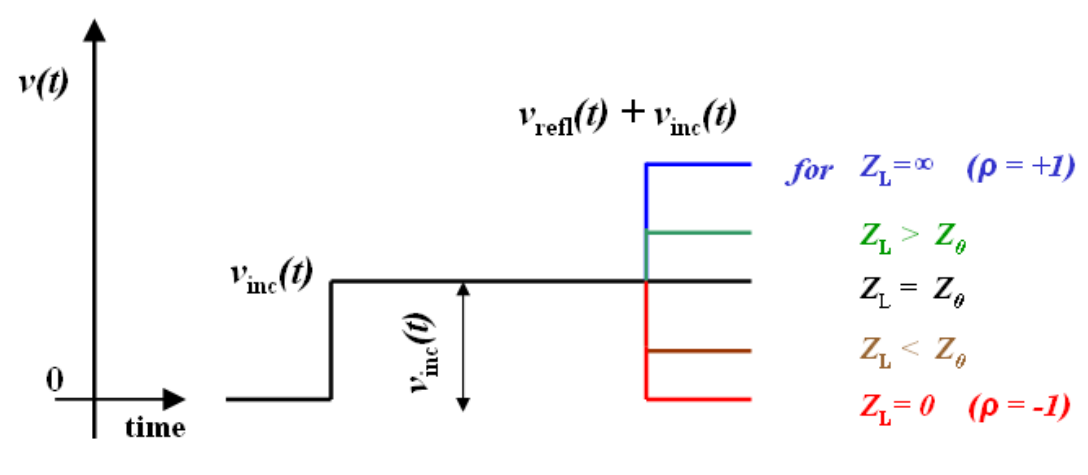
\includegraphics[width=\textwidth,keepaspectratio]{images/onereflectionsample.png}\caption{Znázornění jednoho odrazu na vedení \cite{broadbandreflectometry}.}\label{simpleresponse}\end{figure}

Postupně je možné analyzovat tuto impulzní odezvu tak, že se postupuje od okamžiku budicího signálu, až je nalezen první odraz. Z tohoto odrazu a známého budicího signálu je možné spočítat koeficient odrazu \gls{gama} a prostupu \gls{transmise} v daném místě. Dále postupuje jen množství energie definované koeficientem prostupu a energií obsažené v budicím signálu. Při znalosti této energie, koeficientu odrazu dalšího bodu, kde nastává odraz a koeficientu prostupu prvního odrazu (energie odražená od druhé diskontinuity musí opět projít první diskontinuitou). Takto se postupuje až do konce naměřených dat.

Takto jednoduchý postup ovšem zanedbává vliv vícenásobných odrazů. Přesné výsledky dává pouze pro jeden jediný (resp. první) odraz. Čím více diskontinuit na vedení se nachází, tím více se bude nalezené řešení odchylovat od reality. Pro přesnější analýzu je nezbytné, aby byly uvažovány i vícenásobné odrazy. Je možné mezi jednotlivé kroky analýzy impedančního profilu vložit další analytický krok, který zajistí odečtení vlivu vícenásobných odrazů. Tímto krokem je provedení \acrshort{FDTD} simulace s použitím již získaného částečného impedančního profilu, který je virtuálně bezodrazně zakončen. Výsledkem takovéto \acrshort{FDTD} simulace je odezva takovéhoto úseku vedení (jako průběh odraženého signálu, tak prostupujícího). Nasimulovaný odražený signál je možné odečíst od změřených dat, čímž jsou odstraněny vícenásobné odrazy v již známé části vedení. Dále se pokračuje v analýze tohoto rozdílu měřených a simulovaných dat. Dále se hledá další odraz na vedení a postup se opakuje, dokud není zpracováno celé vedení, nebo dokud energie ve vedení není všechna odražena zpět (platí pro bezeztrátová vedení). Při znalosti fázové rychlosti v daném vedení je možné přepočítat časovou osu na osu prostorovou a odhadnout tedy, kde se nachází diskontinuity.

Dále je možné z těchto odrazů zjišťovat, zda jde o odraz způsobený spojením dvou vedení o rozdílné impedanci (taková diskontinuita se vyznačuje koeficientem odrazu, který se při měření ze dvou stran jeví tak, že má z každé strany koeficient odrazu s jiným znaménkem) nebo o lokální chybu způsobenou například mechanickým poškozením vedení (například navrtaný kabel ve zdi). Taková závada by měla mít z obou stran totožné vlastnosti.

Pro zpracování obecně komplexních koeficientů odrazu (tedy například část vedení, která se chová kapacitně nebo induktivně) by bylo nezbytné vytvořit algoritmus, který by byl schopen rozeznávat v impulsní odezvě nejen čistě reálné odrazy mající v naměřených datech podobu Kroneckerova delta, ale i exponenciální průběhy odpovídající komplexním impedancím, např. na obr. \ref{complexresponse}. Takový algoritmus může být již výrazně náročnější na implementaci, neboť může vyžadovat vícerozměrnou optimalizaci k tomu, aby bylo dosaženo simulací změřené odezvy. Vyvstává také otázka, jak analyzovat, zda jde o přítomnost komplexní impedance na vedení nebo například speciálně zhotovené části vedení, která má spojitý profil impedance, který napodobuje přítomnost komplexní impedance na vedení.

\begin{figure}[htbp]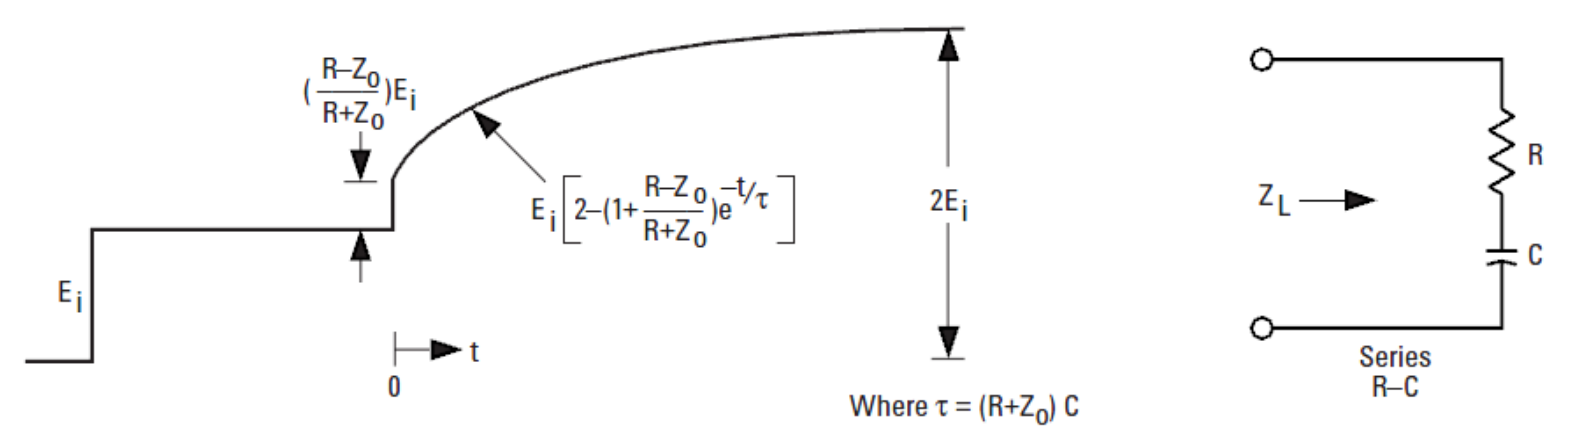
\includegraphics[width=\textwidth,keepaspectratio]{images/samplecomplexresponse.png}\caption{Příklad odezvy na komplexní impedanci na vedení \cite{broadbandreflectometry}.}\label{complexresponse}\end{figure}

Veškeré tyto úvahy se však týkají převážně bezeztrátových vedení, případně vedení, kde je snadné odhalit ztrátové prvky. Obtížné je například měření útlumu měřeného vedení, neboť samotný útlum vedení nemusí být měřitelný jako odraz. Je-li totiž vedení po celé délce homogenní, nevznikají na něm žádné odrazy, avšak vlivem ztrát dielektrika nebo konečnou vodivostí vodičů se část přenášené energie mění na teplo. Další problém je měření části vedení, která se nachází za ideálním útlumovým článkem nebo nějakým prvkem, který transformuje impedanci. Teoreticky není možné odhalit útlumový článek, pokud není možné různými způsoby zakončit vedení, aby byl odhalen vliv zakončení vedení na celkovou odezvu. I při takovém postupu však není možné určit, kde přesně se takový prvek nachází, protože na něm nevzniká žádný odraz, kterým . 

Vzhledem ke značné složitosti této analýzy je zpravidla na reflektometrech a kabelových analyzátorech přítomna pouze funkce detekce první diskontinuity, její polohy a charakteru (zkrat, rozpojení, obecně jiná impedance) \cite{CT-100Bmanual} .

Dalším tématem je měření aktivních prvků, neboť v takovém případě je možné dosáhnout koeficientu odrazu s velikostí větší než 1. V takovém případě je možné analýzou pouze zjistit přítomnost aktivního prvku a jeho odezvu, pro zjištění vlastností takového prvku (například vytvoření modelu tranzistoru) je nezbytné znát vnitřní model takového prvku, což již není úlohou reflektometru. Obecně také může být obtížné analyzovat vedení, na kterém se může nacházet nějaký nelineární prvek (takovým případem může být i například přítomnost vlhkosti ve vedení, která změní impedanci vedení, ovšem nad přibližně 3\,GHz kvůli dielektrické relaxaci přestane mít vliv \cite{relaxationspectroscopy}).

Závěrem této části práce může být tedy konstatování, že je jednoduché odhalit první diskontinuitu (nebo největší, jsou-li ostatní dostatečně malé). Obtížnější je charakterizovat ji, má-li komplexní imepdanci. Mnohem obtížnější je analýza celého vedení, v případě uvažování obecně komplexní impedance může být nemožné získat jednoznačnou analýzu takového vedení, protože může být způsobena jak komplexní impedancí na vedení, tak zvláštně vytvořenému vedení. Přítomnost nelinearit na vedení může zcela znemožnit jakoukoli analýzu nebo způsobit celkovou nesprávnost takové analýzy.

V dalších kapitolách budou rozebrány jednotlivé stavební bloky nezbytné pro konstrukci \acrshort{TDR} a možnosti jejich implementace s přihlédnutím k jednoduchosti fyzické implementace a možností následného zpracovaní naměřených dat.
\chapter{Budicí signál}

\section{Základní požadavky na vlastnosti budicího signálu}
Budicí signál musí splňovat jisté podmínky, aby jej bylo možné použít pro charakterizaci měřeného systému. Následuje formulace základních kritérií pro výběr vhodného budicího signálu.

\begin{itemize}
	\item
	\textbf{Fyzikální realizovatelnost}\\*
	Vzhledem k tomu, že navrhované zařízení musí být realizovatelné, je nezbytné, aby i budicí signál byl fyzikálně realizovatelný. Vzhledem k fyzikálním a praktickým omezením (existence materiálové disperze, nemožnost vytvoření nekonečně velkého proudu, neexistuje bezkapacitní prostředí, neexistuje bezindukční vedení, neexistuje zdroj schopný dodat nekonečné množství energie) není možné vytvořit nespojitý signál. Derivace napětí takovéhoto signálu tedy nemůže být nekonečná. Nespojité signály je tak možné pouze aproximovat spojitými signály, což omezuje například délku a strmost náběžných hran v těchto aproximovaných nespojitostech. Toto fyzikální omezení tedy omezuje frekvenční spektrum takového budicího signálu, zejména jeho šířku.
	
	\item
	\textbf{Spektrální požadavky}\\*	
	Spektrum budicího signálu by mělo být pokud možno konstantní a co nejširší. Neobsahuje-li budicí signál nějakou část spektra, není možné otestovat odezvu systému na tuto část spektra a plně tedy charakterizovat měřený systém. Důvod pro požadavek na rovné spektrum vyplývá z omezeného dynamického rozsahu reflektometru - pokud by část spektra měla příliš malou úroveň, bylo by měření v této části spektra buď více zatížené šumem, případně až neměřitelné. V případě měření některých systémů může být výhodné používat úzkopásmový signál, například při měření části systému nacházející se za pásmovou propustí. V takovém případě by mohla být odezva od části systému za pásmovou propustí maskována mnohem silnějším odrazem od propusti. Jedná se však o specifický případ, který je možné vyřešit i jinými metodami, například redukcí odrazu v nechtěném pásmu \cite{sincgausstdr}. Pro zcela obecné použití by měl být širokopásmový signál vhodnější.
	
	\item
	\textbf{Jednoduchost}\\*	
	Zvolený budicí signál by měl být jednoduchý na vytvoření. Se složitostí signálu může růst složitost zapojení, které by ho mělo generovat, jeho fyzická velikost, případně i náklady na takové zařízení.	

	\item
	\textbf{Rozlišitelnost budicího signálu od odrazů}\\*	
	Budicí signál musí být rozlišitelný od odrazů. Kupříkladu pro buzení periodickým signálem by mělo platit, že odezva měřeného systému na budicí signál musí být kratší než perioda budicího signálu. V opačném případě by se překrývala část odezvy s odezvou od další periody budicího signálu.
\end{itemize}

\section{Výběr budicího signálu a možnosti jeho syntézy}
V této části jsou uvedeny možné podoby budicích signálů a obecné možnosti jejich syntézy. Zároveň jsou zde diskutovány jejich vlastnosti a možnosti následného zpracování. U signálů jsou uvedeny i již existující implementace reflektometrů s těmito budicími signály.

\begin{itemize}
	\item
	\textbf{Diracovo delta}\\*	
	\begin{figure}[htbp]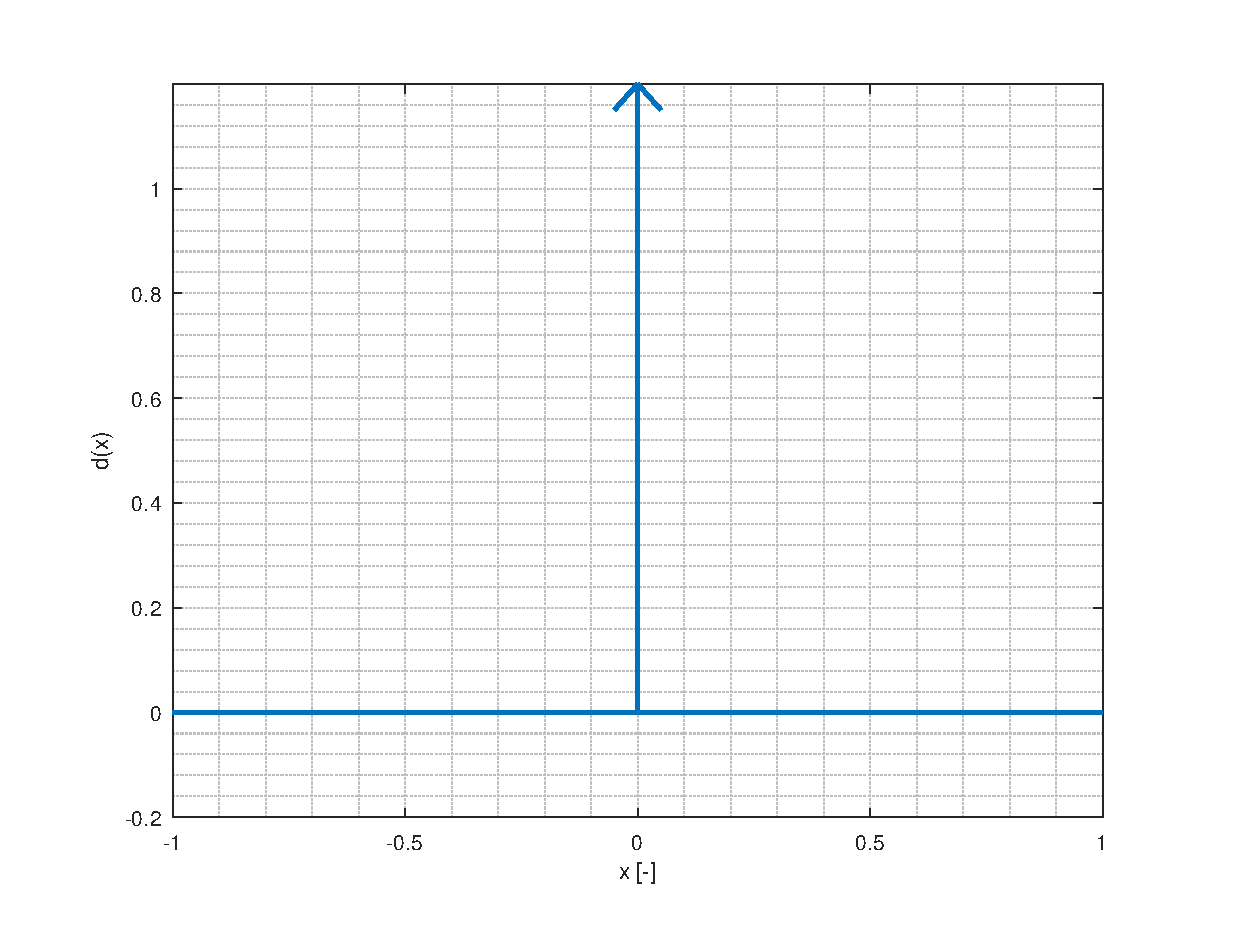
\includegraphics[width=\textwidth,keepaspectratio]{images/dirac.eps}\caption{Diracovo delta.}\label{dirac}\end{figure}		
	Diracovo delta (na obr. \ref{dirac}) je velice jednoduchý signál, který je jedním z ideálních budicích signálů, jeho spektrum je konstanta, má tedy neomezenou šířku frekvenčního pásma. Odezva na Diracovo delta odpovídá impulzní odezvě systému.  Bohužel není fyzikálně realizovatelný, jak je shrnuto v předchozí části textu, neboť je nespojitý a vyžaduje nekonečně rychlé změny napětí a proudu v obvodu. Je tedy možné pouze jej aproximovat, čímž se změní jeho spektrum. Výsledný signál bude mít spektrum odpovídající spektru Diracova delta filtrovaného dolní propustí, čímž se jeho šířka pásma omezí na konečnou velikost. Možná podoba takového signálu je Gaussův pulz na obr. \ref{gauss}.
	
	\begin{figure}[htbp]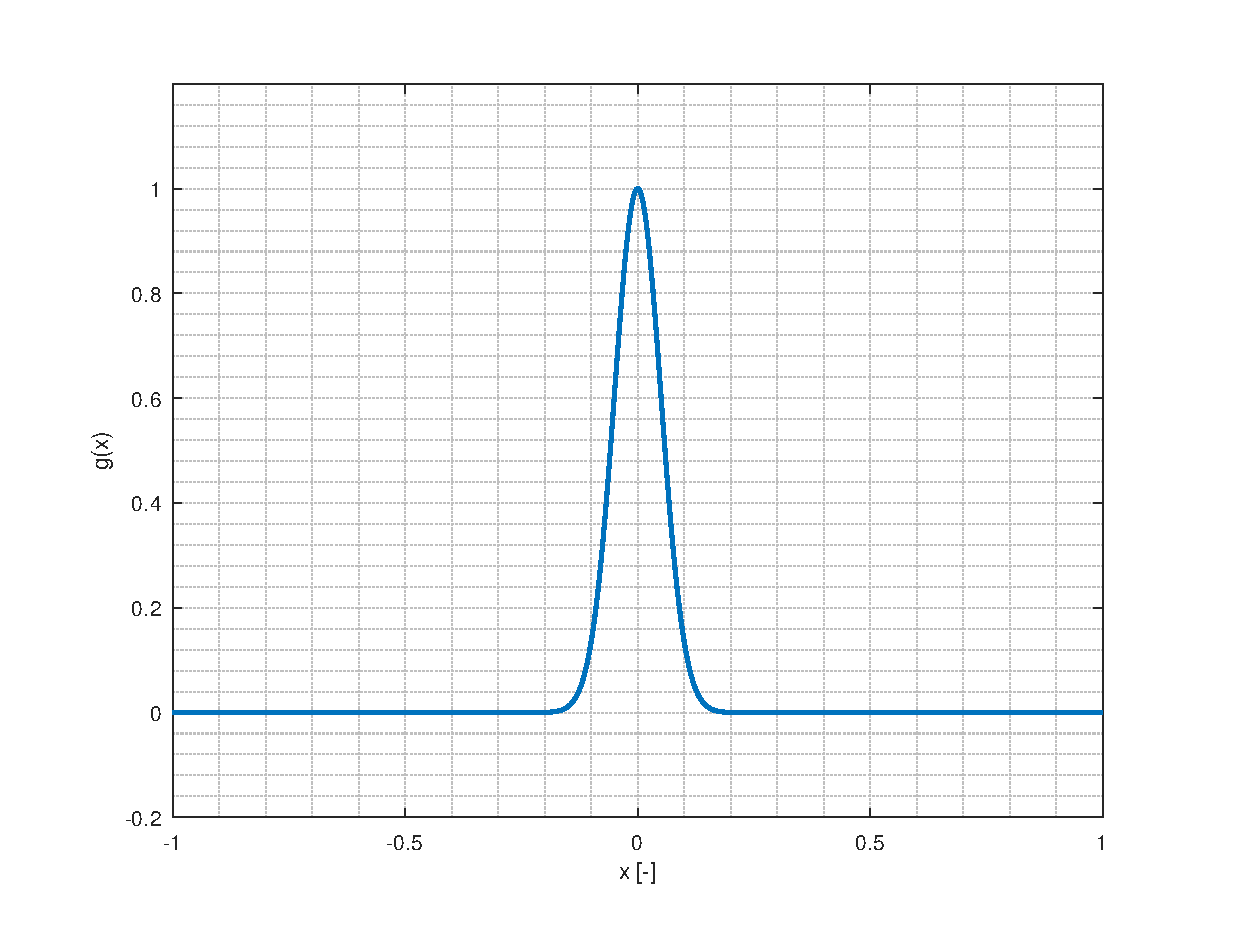
\includegraphics[width=\textwidth,keepaspectratio]{images/gauss.eps}\caption{Gaussův pulz, variance=0.05.}\label{gauss}\end{figure}			
	
	Aproximaci Diracova delta je možné vytvořit pomocí lavinových generátorů impulzů \cite{AN72LT}, \cite{AN94LT}. Pro dosažení impulzu o délce menší než stovky pikosekund je možné použít kombinaci lavinového generátoru impulzů, \acrfull{SRD} a takzvané \gls{clipline} podle obr. \ref{clipline_generator} \cite{S-4manual} \cite{S-1manual}. Takové řešení je však již prostorově náročné, protože vyžaduje zdroj lavinového napětí, transformátory a zkratovací vedení.
	
	\begin{figure}[htbp]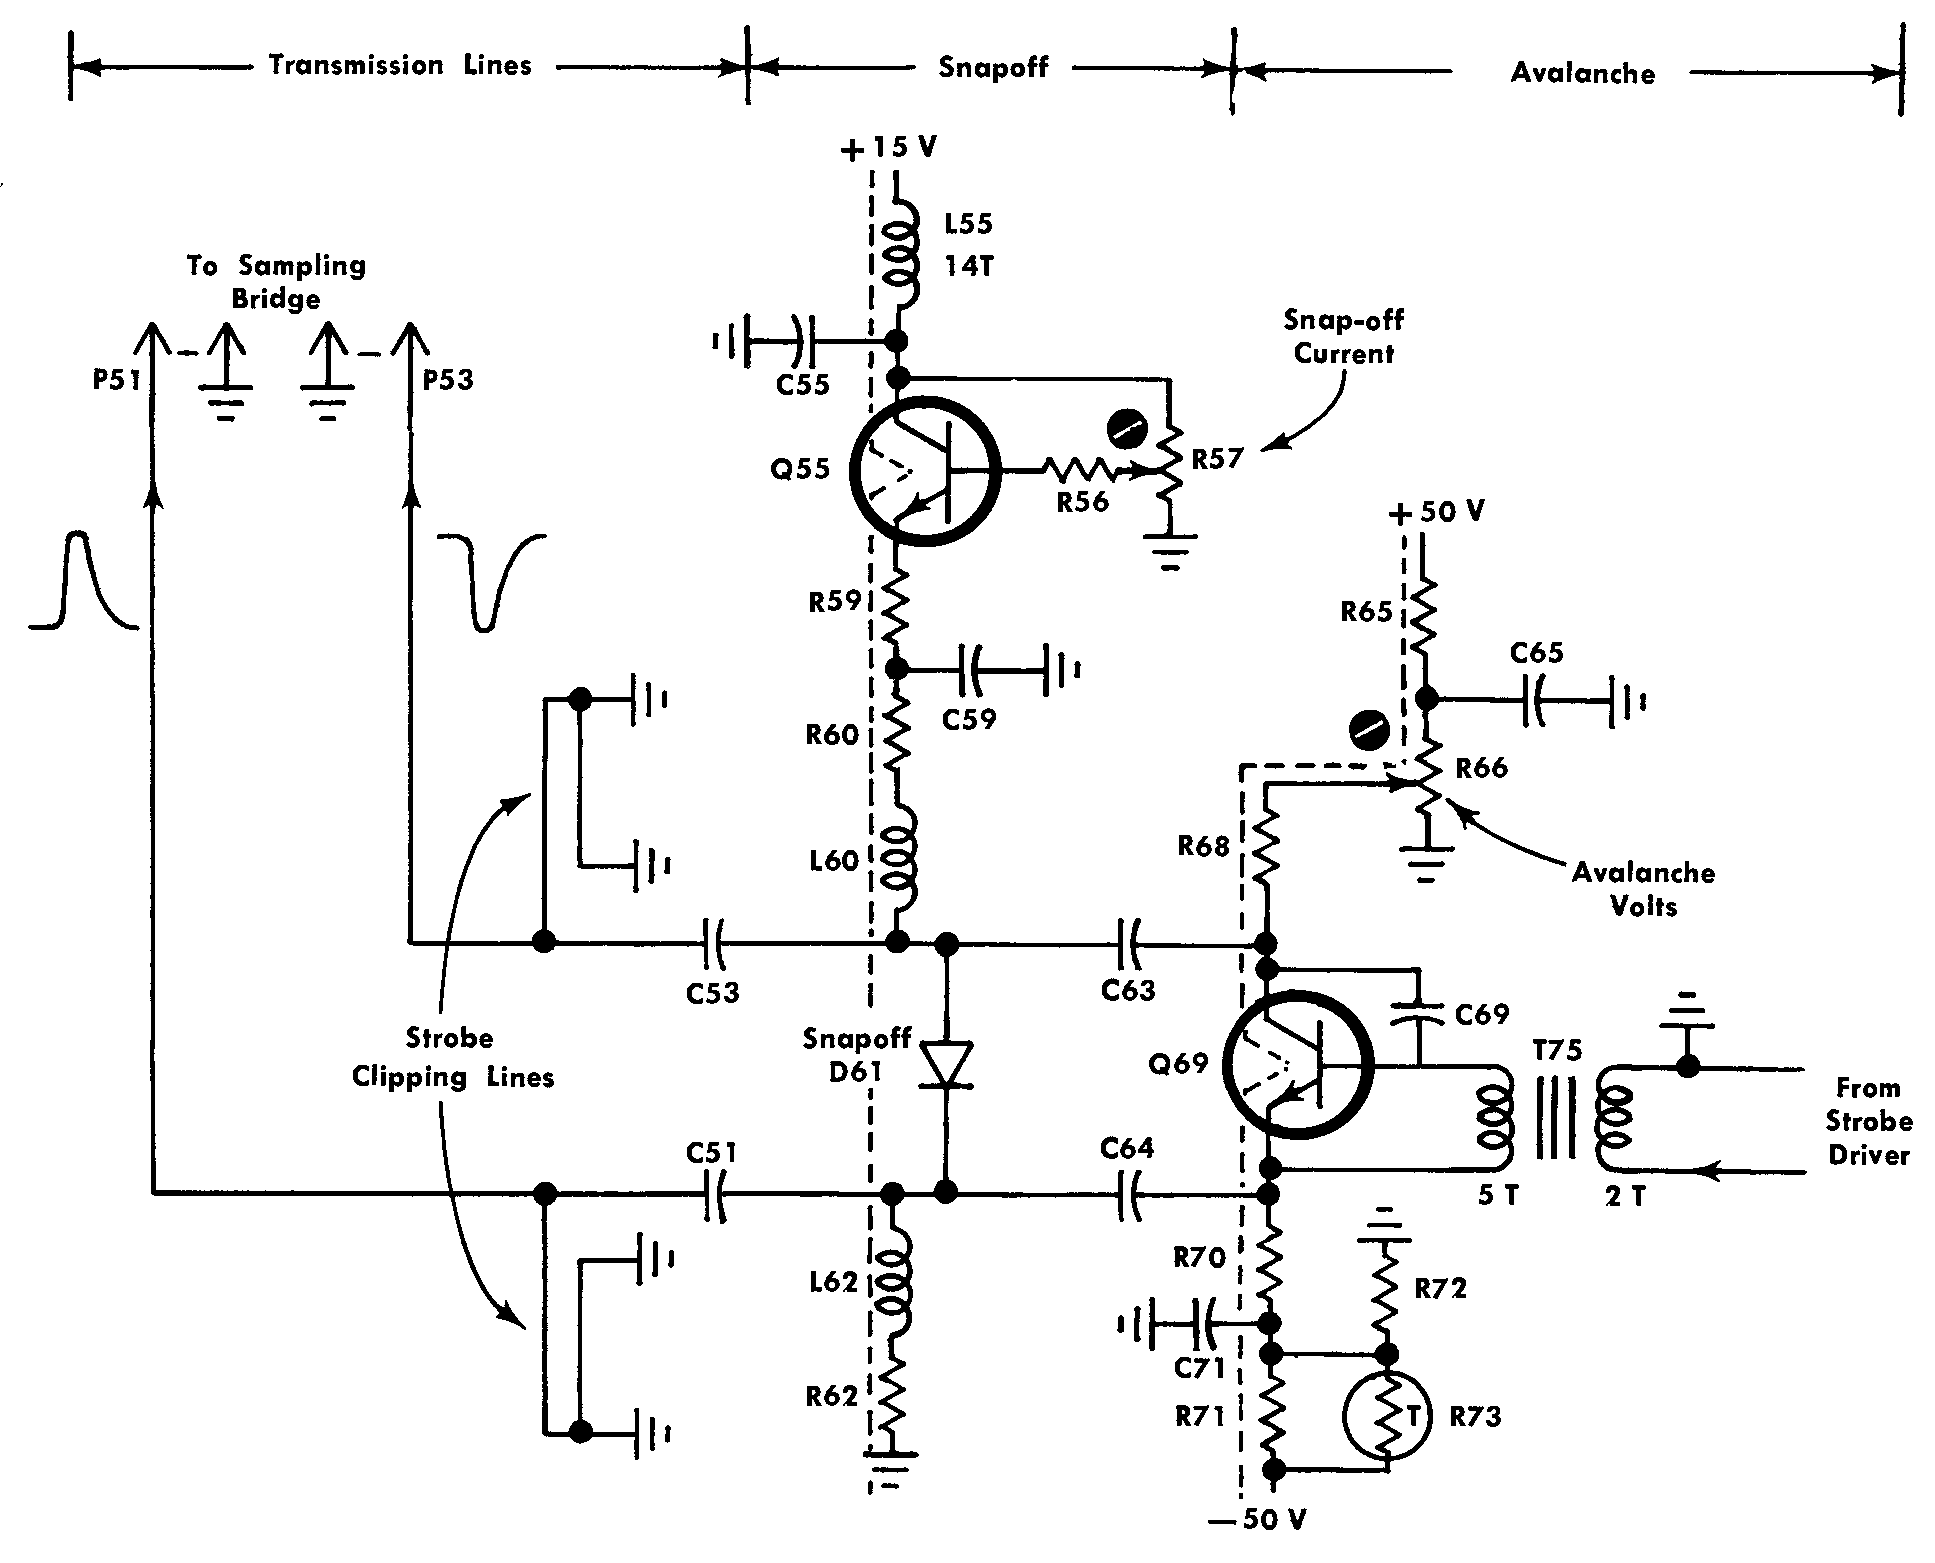
\includegraphics[width=\textwidth,keepaspectratio]{images/clipline_generator.png}\caption{Jehlový generátor s lavinovým generátorem, \acrshort{SRD} a zkratovacím vedením \cite{S-1manual}.}\label{clipline_generator}\end{figure}			
	
	\item
	\textbf{Jednotkový skok}\\*
	\begin{figure}[htbp]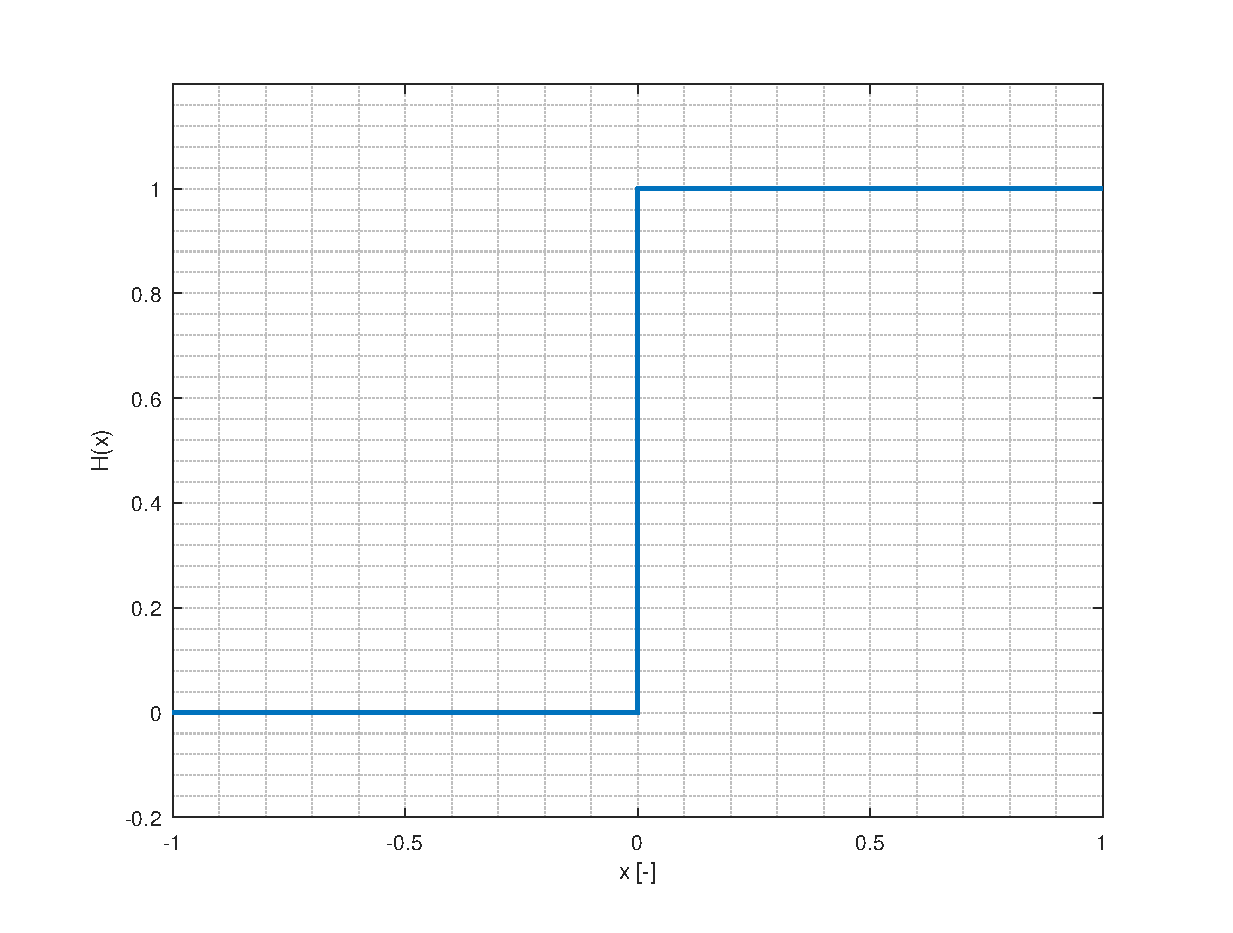
\includegraphics[width=\textwidth,keepaspectratio]{images/unitstep.eps}\caption{Jednotkový skok.}\label{unitstep}\end{figure}		
	Jednotkový skok na obr. \ref{unitstep} odpovídá časovému integrálu Diracova delta
	\begin{equation}
		H(x)=\int_{-\infty}^x \delta(t) dt.
	\end{equation} Opět se jedná o nespojitý signál, který nejde realizovat, jen aproximovat. Reálná aproximace jednotkového skoku je například chybová funkce $\erf(x)$ na obr. \ref{errorfunction}.
	
	\begin{figure}[htbp]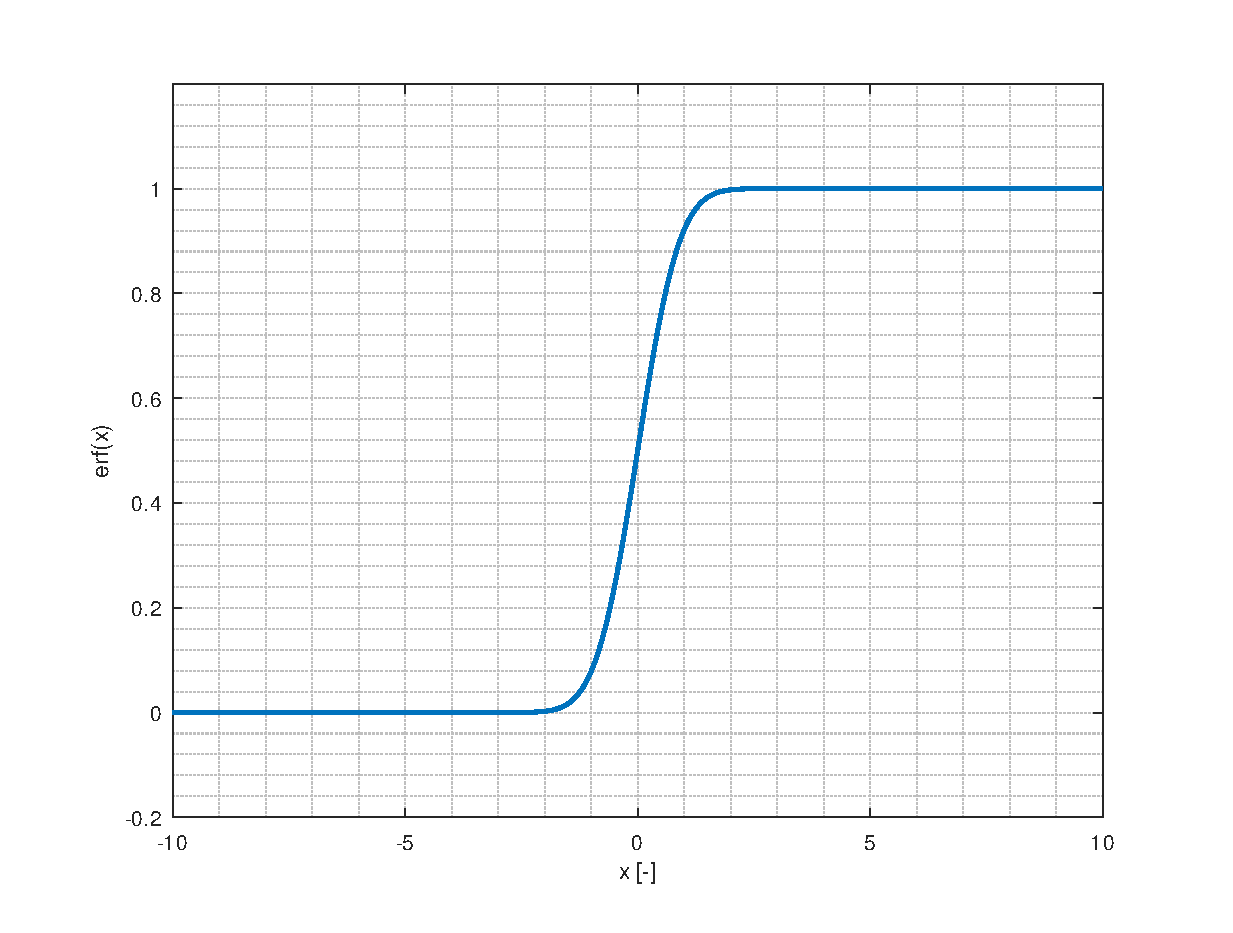
\includegraphics[width=\textwidth,keepaspectratio]{images/erf.eps}\caption{Chybová funkce.}\label{errorfunction}\end{figure}		
		
	Tento budicí signál je možné jednoduše generovat pomocí rychlých logických obvodů. Moderní logické obvody používané pro vysokorychlostní spoje (\acrshort{SATA}, \acrshort{SAS}, \acrshort{USB}\,3, \acrshort{PCI-E}) v řádu jednotek \si{\giga\bit\per\second} již mají náběžné hrany o délce kratší než 100 ps \cite{SY54017datasheet}, \cite{SN75LVCP600Sdatasheet}, \cite{SN65LVPE501datasheet}, \cite{TUSB1002Adatasheet}. Vzhledem k tomu, že pro převod skokové odezvy na impulsní je možné použít jednoduchý vztah
	\begin{equation}
	h(t)=\dv{a(t)}{t},
	\end{equation} a že je syntéza jednotkového skoku možná přímo pomocí logického obvodu, je výhodnější použít jednotkový skok než Diracovo delta. Pravděpodobně z těchto důvodů se u běžných reflektometrů používá právě jednotkový skok jako budicí signál.
	
	\item
	\textbf{Funkce $\boldsymbol{\sinc(x)}$}\\*	
	\begin{figure}[htbp]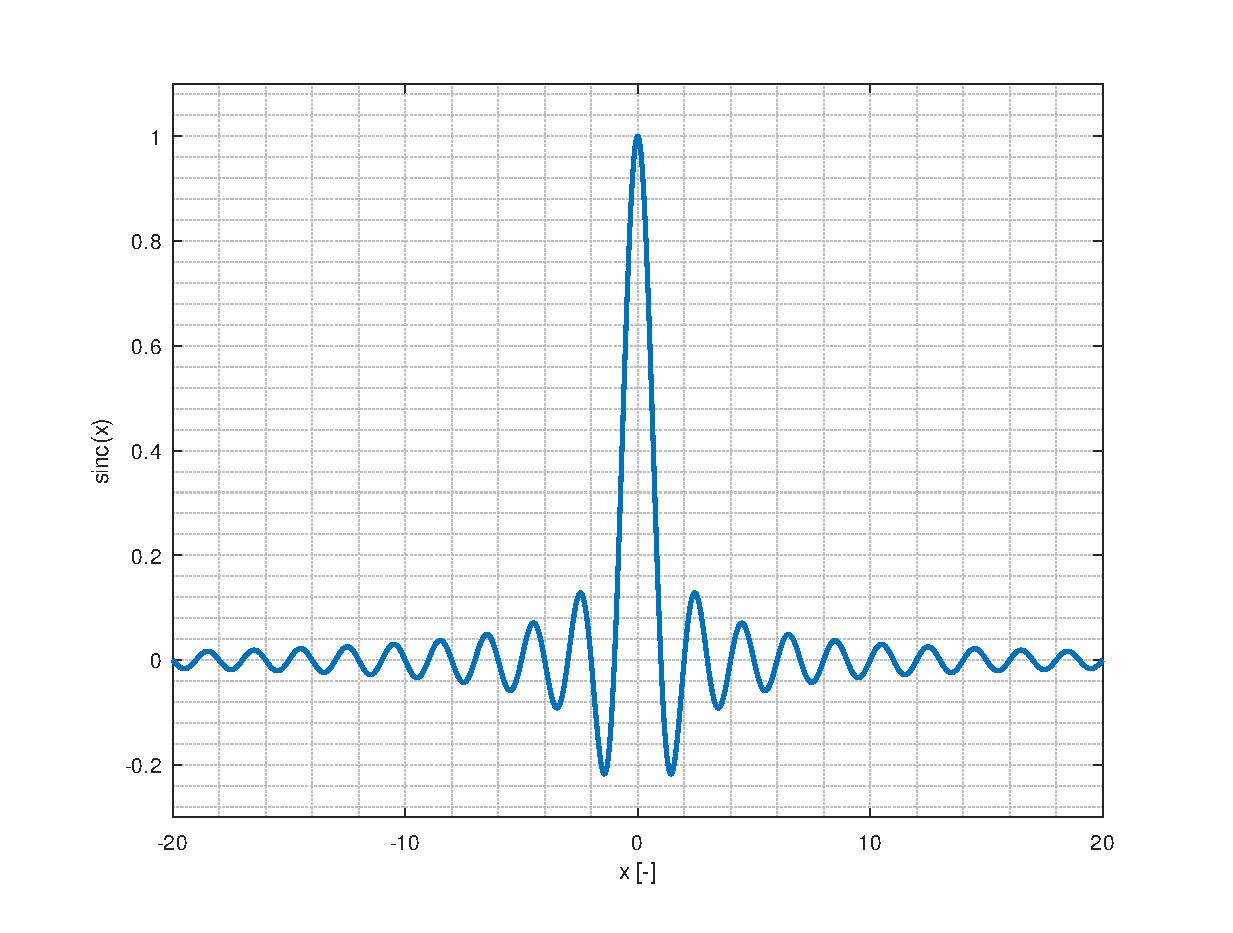
\includegraphics[width=\textwidth,keepaspectratio]{images/sinc.eps}\caption{Funkce $\sinc(x)$.}\label{sinc}\end{figure}		
	
	Další možný budicí signál je funkce $\sinc(x)$ na obr. \ref{sinc}. Tato je již idealizovaně fyzikálně proveditelná (musela by být nekonečně dlouhá), spektrum funkce je konstantní až do mezní frekvence, dále je nulové. Vzhledem k ostrému omezení spektra bohužel není možné změřenou odezvu převést na impulsní odezvu, což komplikuje další zpracování. Autokorelace této funkce je opět $\sinc(x)$, není tedy možné takto jednoduše takovouto odezvu analyzovat.
	
	Pro vytvoření průběhu funkce $\sinc(x)$ je možné modulovat harmonický signál obálkou \cite{sincgausstdr}, ovšem taková obálka by musela být přesně synchronizována s nosným harmonickým signálem, aby nedocházelo ke zkreslení spektra. Jedna z možností, jak přesně simulovat tuto funkci je přímá digitální syntéza, pro tu by ovšem bylo nezbytné použít obvod \acrshort{DDS} s hodinovou frekvencí nejméně dvakrát větší než požadované pásmo, tedy vyšší jednotky GHz. Tento signál nenabízí tedy ani snadnou implementaci, ani vhodné vlastnosti pro použití jako buzení.
	
	\item
	\textbf{Bílý šum}\\*	
	\begin{figure}[htbp]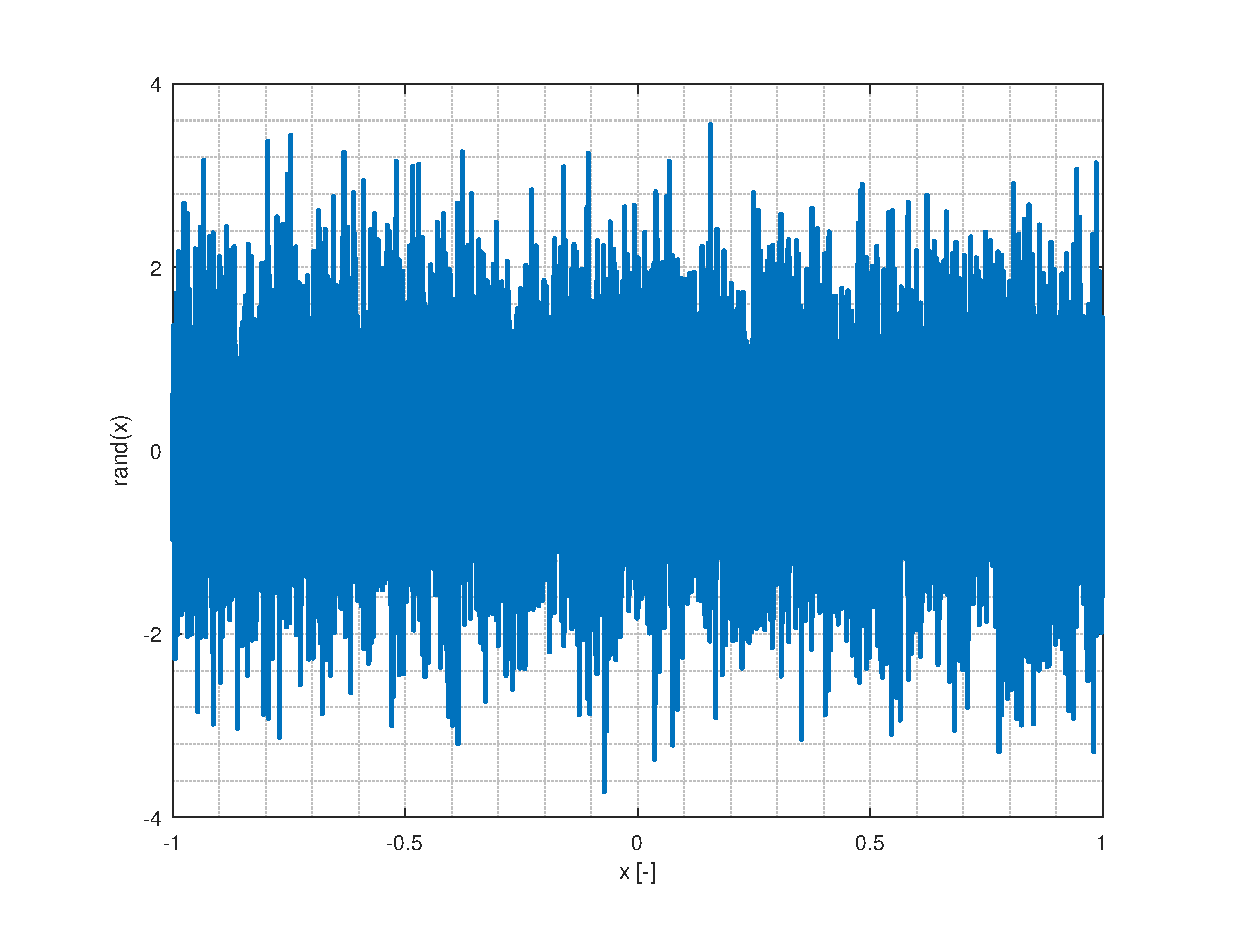
\includegraphics[width=\textwidth,keepaspectratio]{images/whitenoise.eps}\caption{Diskrétní bílý šum.}\label{whitenoise}\end{figure}			
	Při použití bílého šumu (obr. \ref{whitenoise}) je možné získat impulsní odezvu pomocí autokorelace odezvy soustavy. Taková operace zároveň může potlačit nežádaný šum. Pro použití bílého šumu by ale bylo nezbytné, aby budicí šum byl rozlišitelný od šumu nežádaného. Toho lze dosáhnout například zapínáním a vypínáním budicího šumu.
	
	\begin{figure}[htbp]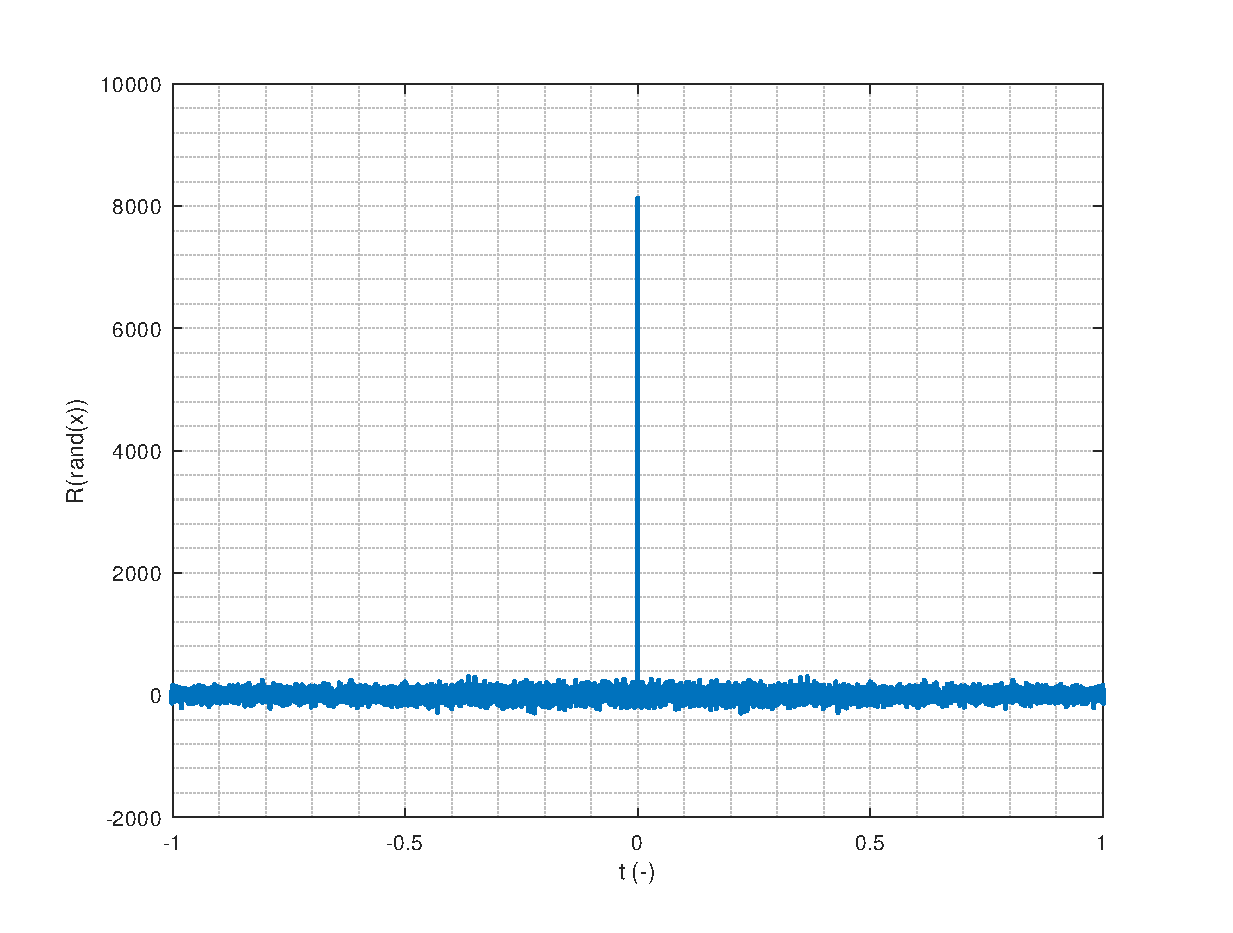
\includegraphics[width=\textwidth,keepaspectratio]{images/whitenoisecorr.eps}\caption{Autokorelace diskrétního bílého šumu z \ref{whitenoise}.}\label{whitenoisecorr}\end{figure}		
	
	Širokopásmový šum je také možné jednoduše vytvořit, například pomocí šumových diod. Modulaci tohoto šumu je možné provádět například pomocí polovodičových mikrovlnných přepínačů. Takový budicí signál je tedy možné jednoduše vytvořit i zpracovávat. Podstatná nevýhoda bílého šumu spočívá v náhodnosti, a z toho vyplývající neperiodicity, kvůli které není možné odezvu systému na takový signál měřit v ekvivalentním čase, jen v reálném čase. Je možné ovšem rovnou měřit autokorelaci, tedy násobením odezvy systému se zpožděnou kopií, kterou je možné vzorkovat pomalu. Autokorelace diskrétního bílého šumu se nachází na obr. \ref{whitenoisecorr}. Bohužel takový přístup vyžaduje použití zpožďovacího vedení s proměnnou délkou, které musí být buď vytvořeno jako mechanický pohyblivý díl nebo jako vedení s velkým množstvím odboček, pak ale je časový krok měření omezen polohou odboček a celková délka měření je omezena délkou vedení \cite{noisedomainreflectometry}. Tuto metodu měření je možné použít pro měření na vedení, na kterém se nachází aktivní zařízení, protože nežádané signály je možné do velké míry odfiltrovat autokorelací. Tato metoda může být tedy výhodná pro měření na předem známých systémech (pevná nehybná vedení), například ve strojích, továrnách, dopravních prostředcích, pro obecné použití se však nezdá být praktická. 
	
	\item
	\textbf{Deterministický šum}\\*
	Za deterministický šum je možné považovat například vedení, které slouží k digitální komunikaci, přičemž obsah posílaných zpráv je známý nebo se tyto zprávy opakují. Pro měření touto metodou je však nezbytná znalost konkrétního měřeného systému \cite{noisedomainreflectometry}, nejde tedy o všeobecně použitelou metodu. 
\end{itemize}

\section{Zvolený budicí signál a obvodové řešení}
Pro jednoduchost syntézy a dobré vlastnosti byl vybrán jednotkový skok. Kvůli rychlostním požadavkům není možné použít klasické logické obvody z řad \acrshort{TTL}, \acrshort{CMOS}, \acrshort{LVCMOS}, \acrshort{HCMOS}, \acrshort{ECL} apod. kvůli velké délce náběžné hrany \cite{subnanosecondgeneratorcomparison}. U těchto technologií je náběžná hrana zpravidla delší než \SI{1}{\nano\second}. Vzhledem k vývoji dnešní techniky, zejména v oblasti vysokorychlostních digitálních přenosů, však již existují velice rychlé logické obvody schopné dosahovat náběžných hran o délce kratší než \SI{100}{\pico\second}. Ve všech dnešních počítačích se již nacházejí technologie jako \acrshort{USB}\,3, \acrshort{HDMI} nebo Display Port, \acrshort{PCI-E}, \acrshort{SATA} nebo \acrshort{SAS} (v serverech), které právě takové obvody vyžadují, díky čemuž jsou dnes již tyto obvody velmi levné. Tyto technologie jsou zpravidla pevně spojeny s metodou signalizace. Používané metody jsou vždy symetrické kvůli šumové odolnosti, používají signalizaci o rozkmitu řádově stovek milivoltů kvůli rychlosti a vyzařování do okolí. 

Běžně používané signalizační technologie:
\begin{itemize}
	\item
	\textbf{\acrshort{LVPECL}}\\*	
		Nízkonapěťová varianta dřívějšího \acrshort{ECL}, která je navíc referencovaná vůči kladnému napájecímu pólu. Vnitřní zapojení je uvedeno na schématu \ref{lvpecl_output}. Jsou navrženy pro připojení k impedanci \SI{50}{\ohm}, bohužel výstupní budiče jsou zapojeny jako emitorové sledovače \cite{lvpecl_vml_cml_lvds_interfacing}, jsou tedy silně nelineární, nemají definovanou impedanci a nejsou tedy vhodné jako budicí obvod do reflektometru, neboť v reflektometru se vyžaduje dobré přizpůsobení měřicího portu, tedy jeho impedance musí být přesně definovaná a konstantní, navíc není žádoucí, aby se měřicí port choval nelineárně.
	
		\begin{figure}[htbp]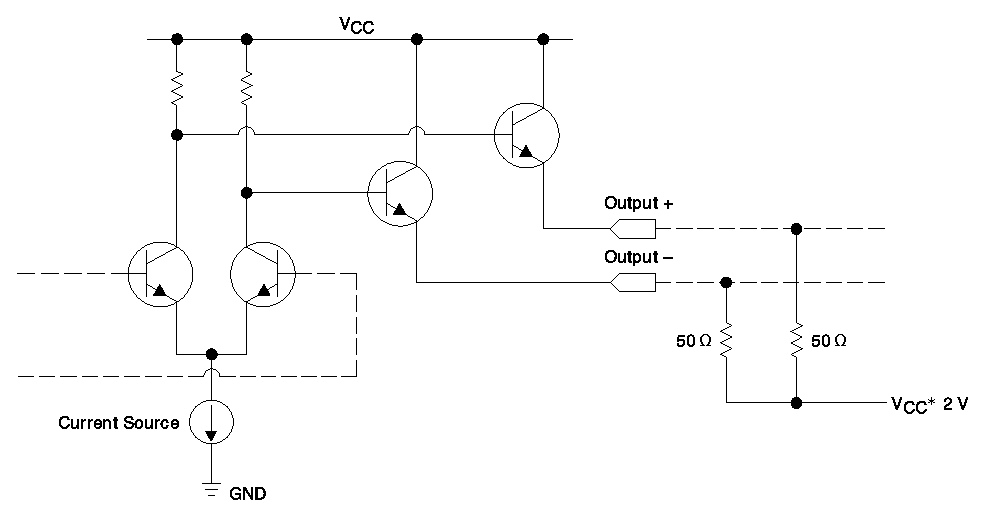
\includegraphics[width=\textwidth,,height=10cm,keepaspectratio]{images/lvpecl_output.eps}\caption{Typické zapojení LVPECL výstupu, převzato \cite{lvpecl_vml_cml_lvds_interfacing}.}\label{lvpecl_output}\end{figure}		
		
	\item
	\textbf{\acrshort{LVDS}}\\*
		Tato signalizace se běžně používá pro přenos obrazu po \acrshort{HDMI} nebo Display Port. Se zmenšeným rozkmitem (\SI{250}{\milli\volt}) se používá i pro \acrshort{SATA} a \acrshort{SAS}.  Vnitřní zapojení je uvedeno na schématu \ref{lvds_output}. Výstupní budiče jsou zapojeny jako \acrshort{CMOS} push-pull budiče \cite{lvpecl_vml_cml_lvds_interfacing} zapojené do drainů tranzistorů, velice podobné jsou i budiče technologie \acrshort{VML} \cite{lvpecl_vml_cml_lvds_interfacing} a \acrshort{HCSL}, očekává se diferenciální zakončení přibližně \SI{100}{\ohm}, případně $2\times\SI{50}{\ohm}$ s pevným středem. Tyto budiče by měly být méně nelineární než \acrshort{LVPECL}, opět však zpravidla není výstupní impedance garantována.
		
		\begin{figure}[htbp]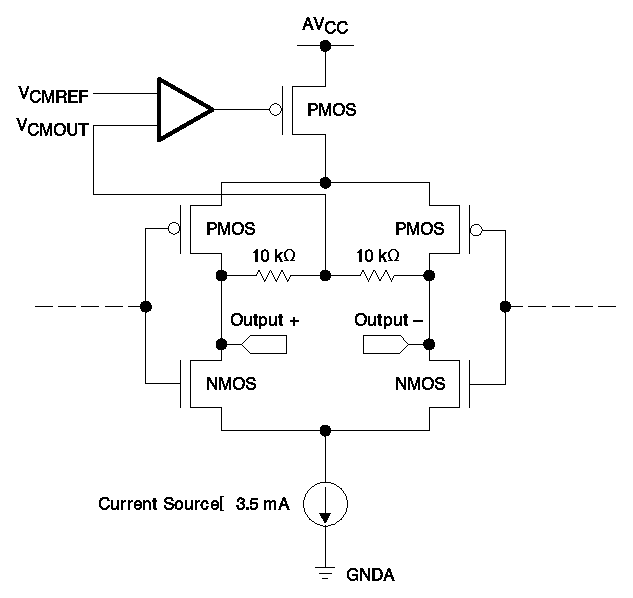
\includegraphics[width=\textwidth,height=8cm,keepaspectratio]{images/lvds_output.eps}\caption{Typické zapojení \acrshort{LVDS} výstupu, převzato z  \cite{lvpecl_vml_cml_lvds_interfacing}.}\label{lvds_output}\end{figure}	

	\item
	\textbf{\acrshort{CML}}\\*
		\acrshort{CML} je signalizační standard používaný zejména pro přenos hodinových signálů. Vnitřní zapojení je uvedeno na schématu \ref{cml_output}. Výstupní budiče jsou zapojeny do kolektoru resp. drainu tranzistoru \cite{lvpecl_vml_cml_lvds_interfacing}, jsou terminovány na \SI{50}{\ohm}, tato hodnota a její tolerance bývá garantována \cite{SY54017datasheet}. Vzhledem k zapojení do kolektoru a interní terminaci je takovýto budič velice dobře přizpůsobený k \SI{50}{\ohm} vedení. 
	
		\begin{figure}[htbp]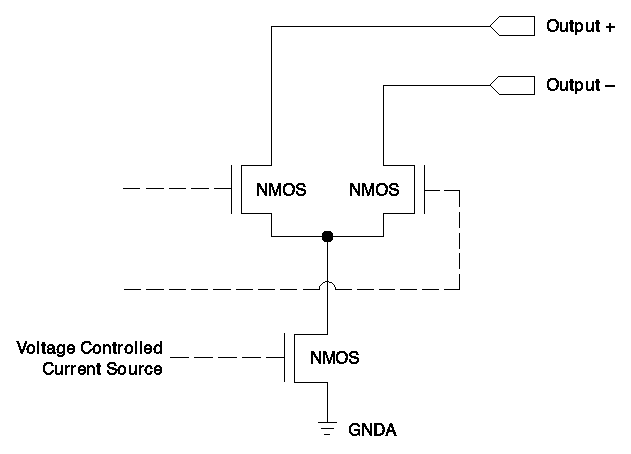
\includegraphics[width=\textwidth,height=8cm,keepaspectratio]{images/cml_output.eps}\caption{Typické zapojení \acrshort{CML} výstupu, převzato z \cite{lvpecl_vml_cml_lvds_interfacing}.}\label{cml_output}\end{figure}		
		
	\item
	\textbf{\acrshort{USB}}\\*
		Další signalizační standard používá například USB, ovšem standard \acrshort{USB}\,3.0 \cite{usb30standard} nespecifikuje přímo technologii, jak této signalizace dosáhnout. Vzhledem k této nejasnosti byly USB redrivery vyřazeny z výběru.
\end{itemize}

Kvůli dobrému přizpůsobení, linearitě a vysoké rychlosti byla zvolena technologie \acrshort{CML}. Další výhodou je, že některým \acrshort{CML} logickým členům je možné měnit napájecí napětí výstupních budičů \cite{SY54020datasheet}. Nejrychlejší dostupné \acrshort{CML} budiče mají typickou délku náběžné hrany \SI{60}{\pico\second} (garantovaný rozsah \mbox{\SIrange{30}{95}{\ps}}, uvádí se pro \mbox{\SIrange{20}{80}{\%}} konečného napětí) \cite{SY54020datasheet}, \cite{SY54017datasheet}. Jsou přímo určeny pro digitální přenosy o rychlostech v řádu \si{\gigabitpersecond}. Tyto budiče tedy splňují požadavek na šířku pásma budicího signálu.
Další důvod pro použití technologie \acrshort{CML} je ten, že \acrshort{SATA}/\acrshort{SAS}/\acrshort{USB} redrivery obvykle obsahují i logiku, která detekuje, zda je přítomen validní signál odpovídající danému přenosovému médiu a v případě, že jej nedetekují, přejdou do úsporného režimu. Přesná metoda, jak je toto spojení detekováno, není zpravidla popsána, hrozilo by tedy, že by se mohl redriver chovat nedefinovaně. Další problém těchto redriverů je to, že jsou určeny pro kompenzaci vlivu frekvenční charakteristiky a ztrát na FR-4 substrátu, takže výsledný signál není prostý obdélníkový průběh, ale složitější stupňovitý průběh jako na obr. \ref{redriver} \cite{SN75LVCP601datasheet}.

		\begin{figure}[H]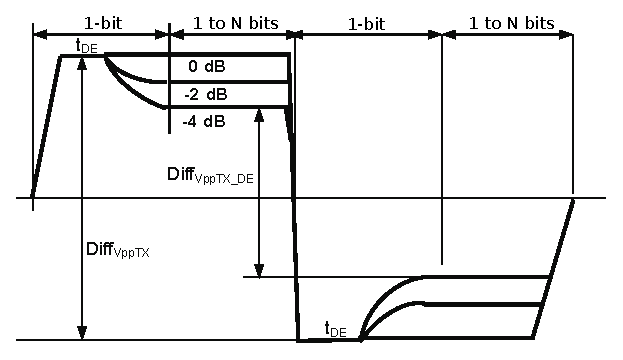
\includegraphics[width=\textwidth,height=6cm,keepaspectratio]{images/redriver.eps}\caption{Výstupní průběh \acrshort{SATA} redriveru \cite{SN75LVCP601datasheet}.}\label{redriver}\end{figure}		

\chapter{Vzorkování odraženého signálu}
Má-li být doržen Nyquistův vzorkovací teorém, je nezbytné vzorkovat budicí a odražený signál na nejméně dvakrát větší frekvenci, než se nachází nejvyšší frekvenční složka měřených signálů. Vybraný zdroj budicího signálu má šířku frekvenčního pásma až \SI{9}{\giga\hertz}, je tedy nezbytné, aby vzorkovač byl schopen vzorkovat alespoň na \SI{18}{\gigasample}. Tento vztah platí při zanedbání frekvenční charakteristiky vzorkovače, který se může chovat jako dolní propust, a tedy minimální vzorkovací frekvence může být nižší. Takovýmto vzorkovacím frekvencím se však blíží jen \quotedblbase folding\textquotedblleft{} ADC a Flash \acrshort{ADC}, které však při takovýchto rychlostech jsou nanejvýš osmibitové, tedy nabízejí dynamický rozsah nanejvýš \SI{48}{\deci\bel}. Nejrychlejší převodníky zatím (v roce 2019) nedosahují vzorkovacích frekvencí ani \SI{10}{\giga\hertz} při dostatčném dynamickém rozsahu. Pro rychlejší vzorkování se používá tzv. \gls{ADCinterleave}, tedy prokládání většího počtu převodníků. Pro přenos a zpracování dat z takto rychlých převodníků jsou potřeba i velmi rychlá FPGA, případně ještě signálové procesory. Tato metoda je ve výsledku v současné době velmi nákladná, navíc má malý dynamický rozsah.

Od doby prvních digitálních osciloskopů se používá technika známá jako vzorkování v \quotedblbase ekvivalentním čase\textquotedblleft . Tato metoda spočívá ve vzorkování periodického signálu přes větší množství jeho period, přičemž postupně se doplňují změřené body, dokud nejsou nalezeny všechny body měřeného průběhu. Hlavní nevýhoda tohoto postupu je nemožnost vzorkování jednorázových signálů (např. šum). Zásadní výhoda tohoto postupu je ovšem možnost částečně potlačit rušení z okolí, jsou-li asynchronní vůči vzorkování. Případně je možné i zvětšit dynamický rozsah, je-li použit rychlý vzorkovač pro navzorkování signálu pro pomalejší vícebitový \acrshort{ADC}. Existují dva základní přístupy, jak provádět toto vzorkování:
\begin{itemize}
	\item
		\textbf{Náhodné vzorkování}\\*		
		Vzorky jsou odebírány neustále, je zaznamenáván časový rozdíl mezi spouštěcí událostí (zde začátek budicího signálu) a nejbližší následující periodou vzorkovacího hodinového signálu. Postupně se tak náhodně doplňují naměřené body, až vznikne dostatečně přesný obraz měřeného signálu. Tato metoda je vhodná například pro osciloskopy, protože zpravidla není možné synchronizovat přesně vzorkovací hodinový signál se spouštěcí událostí.
		
	\item
		\textbf{Postupné vzorkování}\\*
		Vzorky jsou odebírány při každé periodě měřeného průběhu tak, že jednotlivé odebrané vzorky jsou časově seřazeny. Toho se dá dosáhnout fázovým posouváním vzorkovacího hodinového signálu oproti spouštěcí události, což je možné udělat pomocí digitálních zpožďovacích linek nebo tak, že vzorkovací hodinový signál a budicí signál budou mít nepatrně jinou frekvenci \cite{vernierreflectometer}. První řešení může být jednodušší na implementaci, ale zpožďovací linka omezuje krok měření a maximální počet odebraných vzorků \cite{fpgadelaylinereflectometer}, \cite{simpledelaylinereflectometer}. Druhé řešení se dá vytvořit pomocí \acrshort{DDS} \cite{ddsfpgareflectometer} nebo fázového závěsu, který podporuje násobení nebo dělení frekvencí neceločíselným násobkem. Do nedávné doby nebylo řešení pomocí fázových závěsů praktické, protože vyžadovalo fázový závěs pro vytvoření vysokofrekvenční reference a další dva fázové závěsy pro vytvoření dvou rozdílných frekvencí. V posledních letech se však objevily fázové závěsy, které všechny tyto funkce (včetně \acrshort{VCO}) integrují do jediného integrovaného obvodu a prakticky vyžadují pouze kmitočtovou referenci v podobě krystalu nebo krystalového oscilátoru \cite{ADF4350datasheet}, \cite{Si5351datasheet}.
\end{itemize}

\begin{figure}[htbp]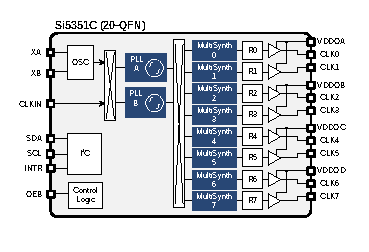
\includegraphics[width=\textwidth,keepaspectratio]{images/si5351_internal_architecture_overview.eps}\caption{Blokové zapojení \acrshort{PLL} Si5351 \cite{Si5351datasheet}.}\label{5351blockdiagram}\end{figure}

Vzhledem k existenci dostupných fázových závěsů umožňujících velkou integraci a miniaturizaci zapojení bylo zvoleno postupné vzorkování pomocí fázového závěsu. Vybraný fázový závěs Si5351 obsahuje v jednom pouzdře dva neceločíselné fázové závěsy \cite{Si5351datasheet}, dva vysokofrekvenční \acrshort{VCO} a osm výstupních neceločíselných děliček. Díky tomuto vývoji v integraci je možné celý hodinový generátor zmenšit do podoby jednoho integrovaného obvodu, jedinou potřebnou externí součástkou je krystal nebo krystalový oscilátor. Neceločíselná část násobiče frekvence umožňuje krok po $2^{{-20}}$ referenční frekvence, je tedy možné měnit podíl frekvencí hodinových signálů s krokem menším než \SI{1}{\ppm}. Při rozdílu frekvencí \SI{1}{\ppm} je počet vzorkovaných bodů celkem 1\,000\,000, což je počet bodů, který je prakticky nedosažitelný se zpožďovacími linkami.

\section{Obvodové řešení vzorkovače}
Pro měření je potřeba vzorkovač s velkou šířkou pásma, nezbytný je i malý \gls{aperturetime}. Historicky se pro tyto účely používaly diodové vzorkovače \cite{S-1manual}, \cite{S-4manual}, příklad takového zapojení na obr. \ref{oscilloscopefrontend}. V dnešní době existují již dostatečně rychlé track-and-hold zesilovače \cite{highspeed_trackhold}, tedy zesilovače, které je možné řízeně zastavit, přičemž na jejich výstupu zůstane napětí, které se tam nacházelo v okamžiku vypnutí zesilovače. Mezní kmitočet běžně prodávaných typů se pohybuje v současné době okolo \SI{8}{\giga\hertz}. Bohužel jsou oproti diodovým vzorkovačům velice nákladné.

\begin{figure}[htbp]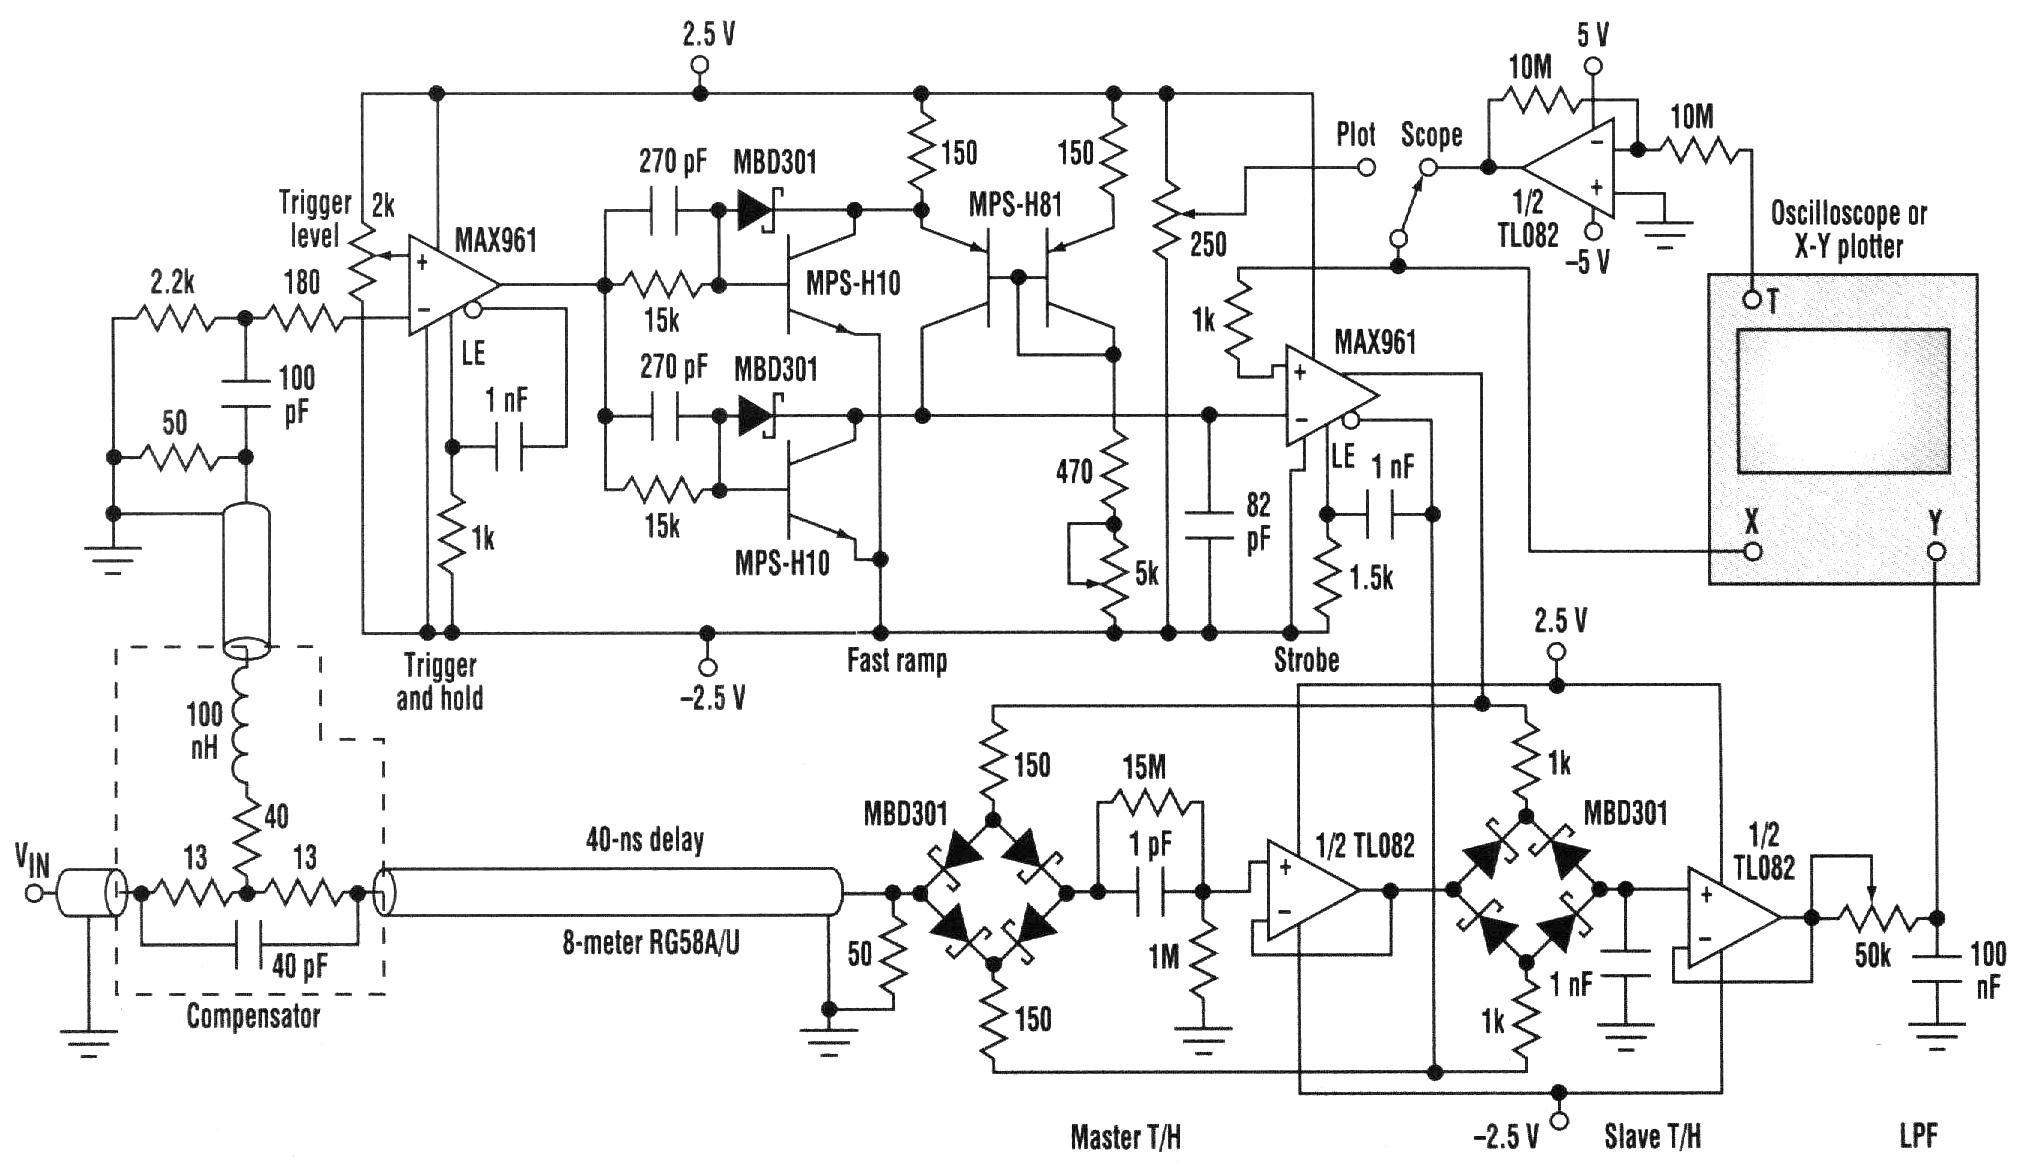
\includegraphics[width=\textwidth,keepaspectratio]{images/oscilloscopefrontend.png}\caption{Praktické zapojení vzorkovacího můstku do \SI{1}{\giga\hertz}, převzato z \cite{oscilloscopefrontend}.}\label{oscilloscopefrontend}\end{figure}		

Diodové vzorkovače se používaly již v prvních digitálních osciloskopech a reflektometrech, protože jejich šířka použitelného frekvenčního pásma je omezena téměř výhradně sériovým dynamickým odporem diodového vzorkovače, velikostí vzorkovacího kondenzátoru a aperturovým časem. Aperturový čas je doba, po kterou trvá rozepnout vzorkovač, závisí zejména na kapacitě diody (bariérové i difuzní) a zapojení budiče, který diody rozepíná. Pro toto použití jsou zejména vhodné Schottkyho diody kvůli malé paralelní kapacitě a možnosti velice rychle diody rozepnout. Speciálně pro použití ve vzorkovačích se vyrábí přesné vyvážené diodové čtveřice \cite{HSMS282xdatasheet}, které umožňují silně potlačit průnik vzorkovacího buzení do vzorkovaného signálu, což umožňuje použití velmi malých vzorkovacích kondenzátorů, a tedy velkou šířku užitečného frekvenčního pásma takového vzorkovače.
	
\chapter{Separace budicího a odraženého signálu}
Pro potřeby zpracování změřených dat je nezbytné separovat budicí signál od jeho odrazů. Takovou separaci je možné provádět buď hardwarově v době měření nebo až během zpracování změřených dat. Cílem je dosáhnout toho, aby byly tyto dva signály zcela oddělené (či oddělitelné při zpracování). Možné metody separace:
\begin{itemize}
	\item
	\textbf{Směrová odbočnice}\\*	
	\begin{figure}[htbp]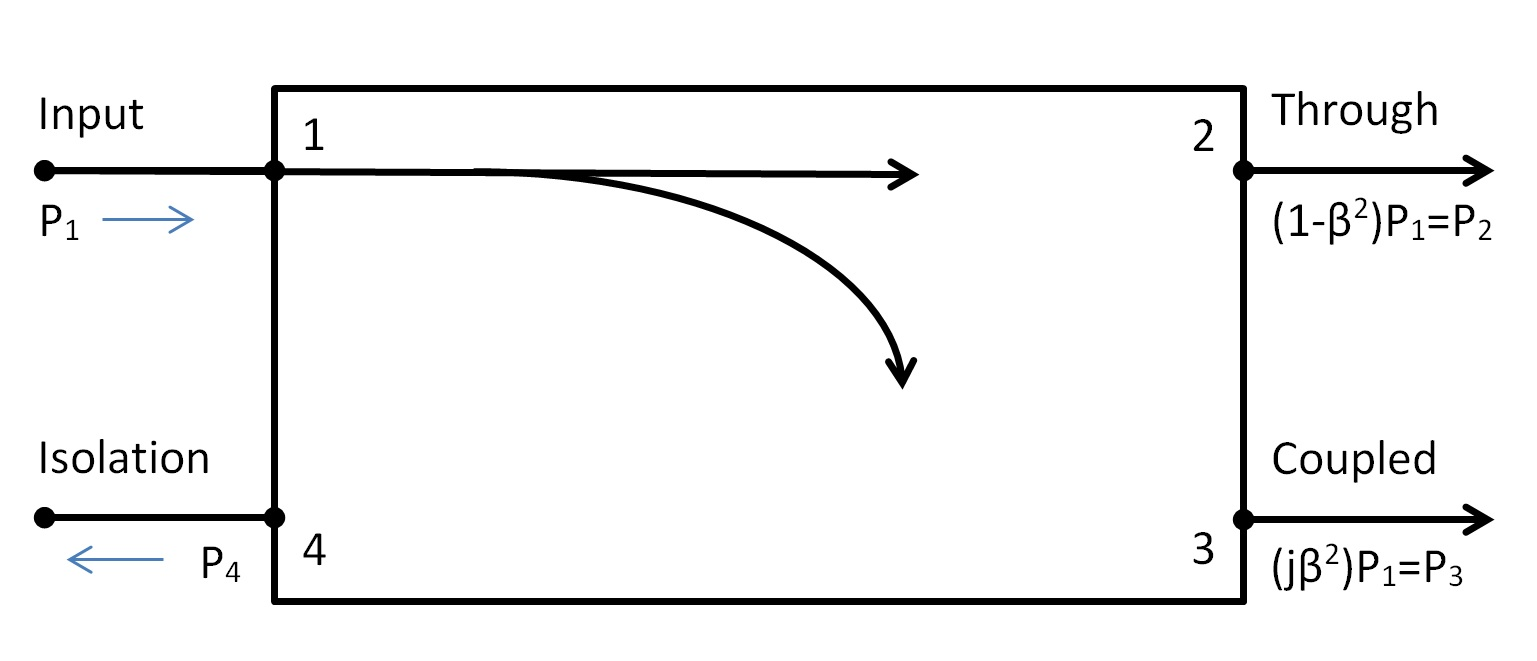
\includegraphics[width=.8\textwidth,keepaspectratio]{images/directionalcoupler.png}\caption{Směrová odbočnice, převzato z \cite{widebandcouplers}.}\label{directionalcoupler}\end{figure}	

	Pomocí tradičních odbočnic jako na obr. \ref{directionalcoupler} je možné provádět separaci s velkou izolací nechtěného signálu, ovšem nesplňují požadavek na šířku zpracovávaného pásma \cite{widebandcouplers}. Problematická je také skutečnost, že s rostoucí šířkou použitelného pásma odbočnice obvykle klesá směrovost odbočnice. Dochází tedy pouze k částečné separaci, další separační krok by byl nezbytný během zpracování naměřených dat.
	
	\item
	\textbf{Odporový můstek}\\*	
	\begin{figure}[htbp]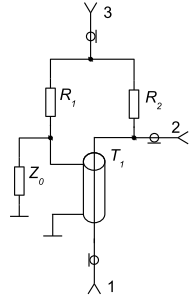
\includegraphics[width=\textwidth,height=5cm,keepaspectratio]{images/resistivebridge.png}\caption{Odporový směrový můstek, převzato z \cite{resistivedirectionalbridge}.}\label{resistivebridge}\end{figure}	
	Pomocí odporových můstků je možné provádět separaci signálů s velmi velkou šířkou pásma, např. v \cite{resistivedirectionalbridge} a obr. \ref{resistivebridge} uveden můstek pro pásmo \SI{300}{\kilo\hertz}--\SI{13.5}{\giga\hertz}. Opět ovšem nejsou signály plně separovány, je nezbytný další separační krok během zpracování.
	
	\item
	\textbf{Časové oddělení}\\*	
	Pokud má budicí signál tu vlastnost, že má omezenou délku, po kterou se mění a mimo ni je konstantní (vybraný jednotkový skok tuto vlastnost splňuje), je možné jej od odrazů separovat tak, že je časově posunut vůči odezvě systému. Toho je možné dosáhnout například použitím dokonalého vedení bez odrazů, které se zapojí mezi bod měření a měřený systém. Jeho délka musí být minimálně taková, aby se nemohla nikdy překrývat nekonstantní část budicího signálu s odrazy. Pokud je v naměřených datech známá poloha budicího pulzu (nebo je-li možné jej spolehlivě identifikovat), je možné naměřená data rozdělit na část buzení a část odpovědi měřeného systému. První část pak může sloužit ke korekci frekvenční charakteristiky změřené odezvy systému a odhadu šumového spektra. Známe-li i přesnou délku prodlužovacího vedení (hrubě z návrhu zařízení, přesně pomocí kalibrace), je možné provést kalibraci měřicí roviny. Při použití této metody separace stačí vzorkování pouze jednoho průběhu, snižuje tedy počet potřebných vzorkovačů ze dvou (nebo více) na jeden. Z toho také vyplývá, že měřená data nejsou zatížena chybou, která by mohla vzniknout vzhledem k rozdílným vlastnostem jednotlivých vzorkovačů.
	
	Na obrázku \ref{separableunitstep} je znázorněna odezva na chybovou funkci. Buzení se nachází v čase $t=0$, odezva v čase $t=0.5$. Průběh budicí funkce je předem známý, nekonstantní část průběhu se nepřekrývá s odezvou, je tedy možné je v časové oblasti $t\in (0;0.5)$ rozdělit na dva samostatné průběhy.

\begin{figure}[htbp]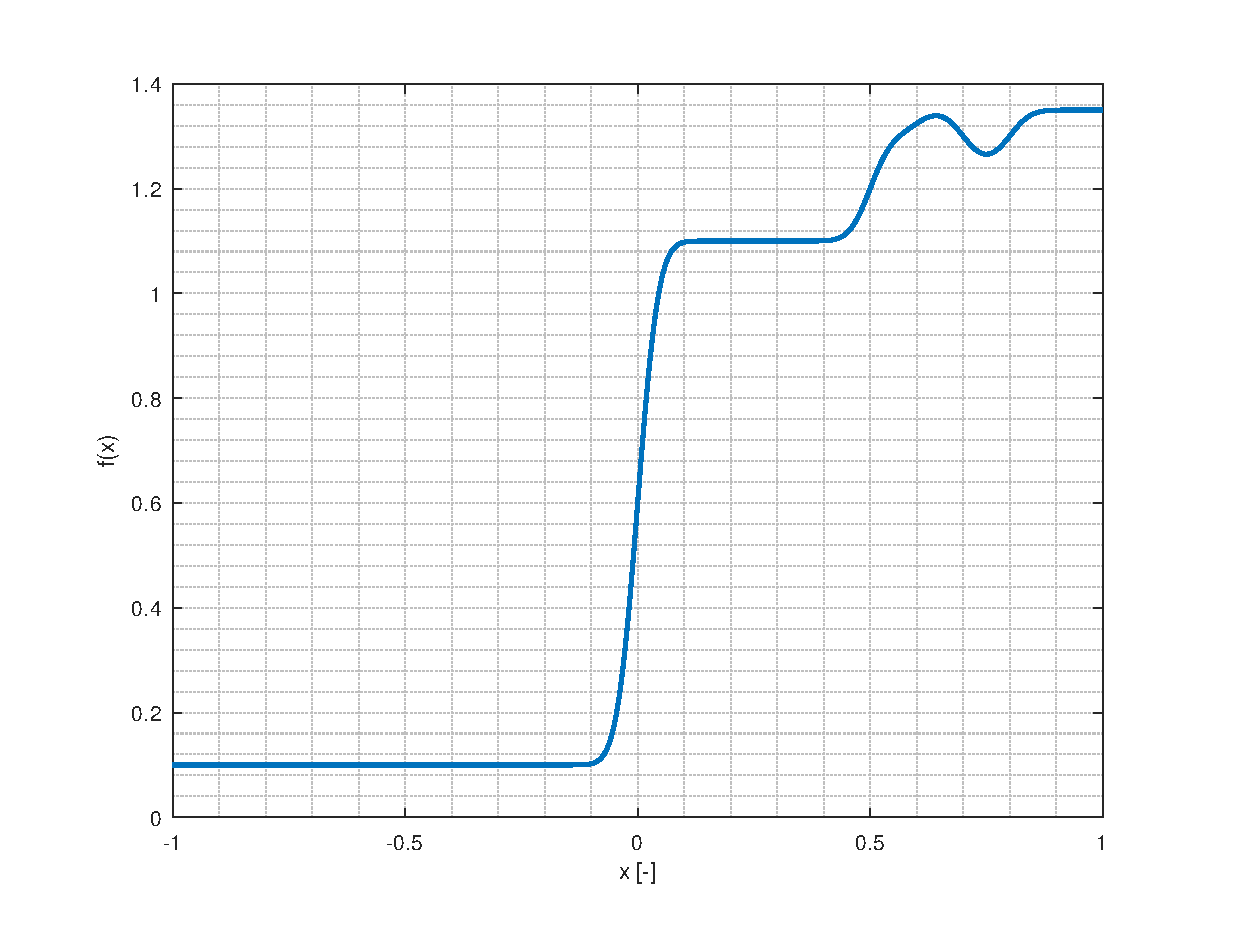
\includegraphics[width=\textwidth,keepaspectratio]{images/separableunitstep.eps}\caption{Časově oddělitelná odezva na jednotkový skok.}\label{separableunitstep}\end{figure}	
\end{itemize}

Pro vybraný budicí signál (jednotkový skok) je tedy možné provést separaci od odrazů zpožďovacím vedením a vhodným rozdělením naměřených dat na dvě části. Toto řešení se jeví jako obvodově i výpočetně nejjednodušší z uvažovaných metod separace.
\chapter{Rozšíření dynamického rozsahu, potlačování šumu a rušení}
Pro co nejpřesnější měření je nezbytné dosáhnout co největšího SNR (signal to noise ratio). Prvním limitujícím faktorem je dynamický rozsah ADC. V případě měření v reálném čase by bylo možné použít nanejvýš osmibitové převodníky, které mají dynamiku přibližně \SI{48}{\deci\bel} podle vztahu \ref{equation_dynamic_range}.
\begin{equation}
	 DR_n=20\log\left(2^n-1\right)
	 \label{equation_dynamic_range}
\end{equation}
Pro nižší rychlosti jsou dostupné již ADC s vyšší přesností, někdy již integrované přímo do mikrokontrolérů. Běžně se integrují převodníky až do \SI{1}{\megasample} při rozlišení 12~bitů, tedy s dynamickým rozsahem přibližně
\begin{equation}
	DR_{12}\doteq \SI{72}{\deci\bel}
\end{equation}

Pro aplikace ve zvukové technice jsou pak dostupné šestnáctibitové až dvacetičtyřbitové převodníky (obvykle do \SI{96}{\kilosample}) s dynamikou od 
\begin{equation}
	DR_{16}\doteq \SI{96}{\deci\bel}
\end{equation} až do
\begin{equation}
	DR_{24}\doteq \SI{144}{\deci\bel}
\end{equation}
 Druhý údaj je však pouze teoretický, převodníky sice nabízejí tento počet bitů, ovšem jejich vlastní šum zpravidla omezuje použitelný rozsah na méně než \SI{100}{\deci\bel}. Přesné \SI{24}{\bit} převodníky, které mají skutečně dynamický rozsah odpovídající počtu bitů, vzorkují zpravidla nanejvýš na desítkách \si{\hertz}. Takové rychlosti jsou však pro použití v reflektometru příliš pomalé, neboť změření odezvy systému by bylo velice zdlouhavé.

Vzhledem k rychlosti se zdají být použitelné nanejvýš \SIrange{12}{16}{bitové} převodníky. Existují ovšem metody rozšíření dynamického rozsahu, zpravidla spoléhající na zkreslení měřených dat nelineární funkcí, která umožní navzorkovaná data inverzní funkcí převést zpět na původní signál, přičemž ale nedojde ke ztrátě přesnosti, nýbrž k jejímu zlepšení v určité části převodní charakteristiky. Pro účely telefonie se v minulosti používaly například komprese definované ve standardu G.711 od ITU-T. Tyto komprese umožňovaly komprimovat logaritmicky enkódovaná data z 14~bitů na 8, přičemž uživatel po dekompresi pozoroval výrazně menší zkreslení, než k jakému by došlo, pokud by bylo použita přímo osmibitová kvantizace.

Pro účely měření vysokofrekvenčních signálů se vyrábí logaritmické detektory s rozsahem až \SI{100}{\deci\bel} \cite{AD8309datasheet} \ref{ad8309function}. Pro nízké frekvence poskytuje např. detektor AD8309 \SI{85}{\deci\bel} dynamického rozsahu při toleranci $\pm \SI{1}{\deci\bel}$, tolerance je zakreslena v grafu \ref{ad8309error}. Logaritmus je prostá funkce, je tedy možné spočítat její inverzní funkci. Podle \ref{ad8309function} odpovídá vstupnímu rozsahu \SIrange{-70}{10}{\deci\bel m} výstupní rozsah o velikosti \SI{1.5}{\volt}. Při uvažování převodníku s referencí \SI{3.3}{\volt} a rozlišení 12~bitů odpovídá nejmenší měřitelný rozdíl napětí převodníkem \SI{0.8}{\milli\volt}, což s detektorem odpovídá vstupnímu rozlišení přibližně \SI{0.043}{\deci\bel}. Kombinací takového detektoru s dvanáctibitovým převodníkem a proložením dat získaných z lineárního a logaritmického měření je možné vytvořit převodník, který se přesností blíží rychlému šestnáctibitovému převodníku.

\begin{figure}[htbp]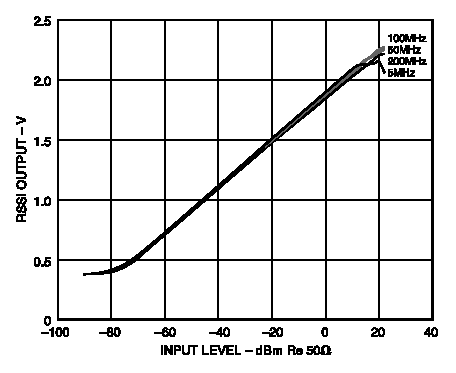
\includegraphics[width=0.8\textwidth,keepaspectratio]{images/AD8309_function.eps}\caption{Převodní funkce logaritmického detektoru AD8309 \cite{AD8309datasheet}}\label{ad8309function}\end{figure}	

\begin{figure}[htbp]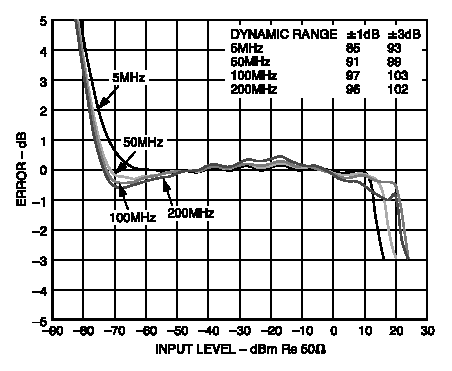
\includegraphics[width=0.8\textwidth,keepaspectratio]{images/AD8309_error.eps}\caption{Chyba převodní funkce logaritmického detektoru AD8309 \cite{AD8309datasheet}}\label{ad8309error}\end{figure}

Pro potlačení šumu v měřeném průběhu je možné použít velké převzorkování signálu a aplikovat na tato data filtr pro potlačení šumu mimo užitečné pásmo. Dále je možné měřený průběh opakovaně měřit a statisticky zpracovávat (buď jednoduchým průměrem nebo např. Kalmanovými filtry).

Použitím měření v ekvivalentním čase je také možné redukovat rušení z okolí za předpokladu, že žádný násobek tohoto rušivého signálu není přesně roven vzorkovacímu kmitočtu. Pak se toto rušení projeví jako šum, který je možné odstranit či alespoň potlačit metodami zmíněnými v předchozím odstavci. V opačném případě je možné rušení potlačit pouze tak, že se provede měření s jinou vzorkovací frekvencí.
\chapter{Navržené blokové zapojení reflektometru}
V předchozích kapitolách byly vysvětleny technologie, které byly uvažovány pro návrh architektury jednoduchého reflektometru a následně byly z nich vybrány ty nejvhodnější nebo nejjednodušší na implementaci. Pro jednotlivé části reflektometru tedy budou použity tyto stavební bloky:
\begin{itemize}
	\item
	\textbf{Buzení}\\*
	Pro buzení bude použito buzení aproximovaným jednotkovým skokem pomocí budiče technologie \acrshort{CML}, kterým je možné dosáhnout aproximace s náběžnou hranou o délce kratší než \SI{100}{\pico\second}, typicky okolo \SI{60}{\pico\second}, tedy s užitečnou šířkou pásma v jednotkách \si{\giga\hertz}. Výstup je dobře přizpůsoben pro použití v \SI{50}{\ohm} systémech.
	
	\item
	\textbf{Separace budicího a odraženého signálu}\\*	
	Pro separaci buzení od odezvy systému bude použito prodlužovací vedení jako metoda pro dosažení časového posunu. Samotná separace bude probíhat až z navzorkovaných dat během zpracování.
	
	\item
	\textbf{Vzorkování}\\*	
	Data budou sbírána pomocí postupného vzorkování v ekvivalentním čase pomocí vyvážených diodových můstků. Touto metodou je možné vzorkovat měřený signál pomocí pomalých převodníků s větším dynamickým rozsahem a přesností, je také možné potlačit ruchy z okolí. Byla navržena metoda pro měření s dynamickým rozsahem nejméně \SI{80}{\deci\bel}.
	
	\item
	\textbf{Generování signálů pro řízení reflektometru}\\*	
	Pro řízení jednotlivých částí reflektometru bude použita \acrshort{PLL} Si5351, která disponuje 8 výstupy, které je možné konfigurovat jako diferenciální výstupy. Jednotlivé výstupy mohou mít neceločíselné vzájemné poměry frekvencí (krok nastavení je menší než \SI{1}{ppm}), je možné dosáhnout vzorkování s krokem menším než \SI{100}{\pico\second}, tedy ekvivalentní vzorkovací frekvence větší než \SI{10}{\gigasample}. Díky proudovým výstupům je možné ji přímo propojit jak se vstupy \acrshort{CML} logických prvků, tak ji použít pro spínání diodových vzorkovačů. Je možné i vygenerovat synchronizační hodinový signál pro mikrokontrolér, aby se provádělo vzorkování v přesně stanovený čas.
\end{itemize}

Z těchto jednotlivých prvků je tedy již možné navrhnout základní blokové zapojení navrhované architektury.

\begin{figure}[htbp]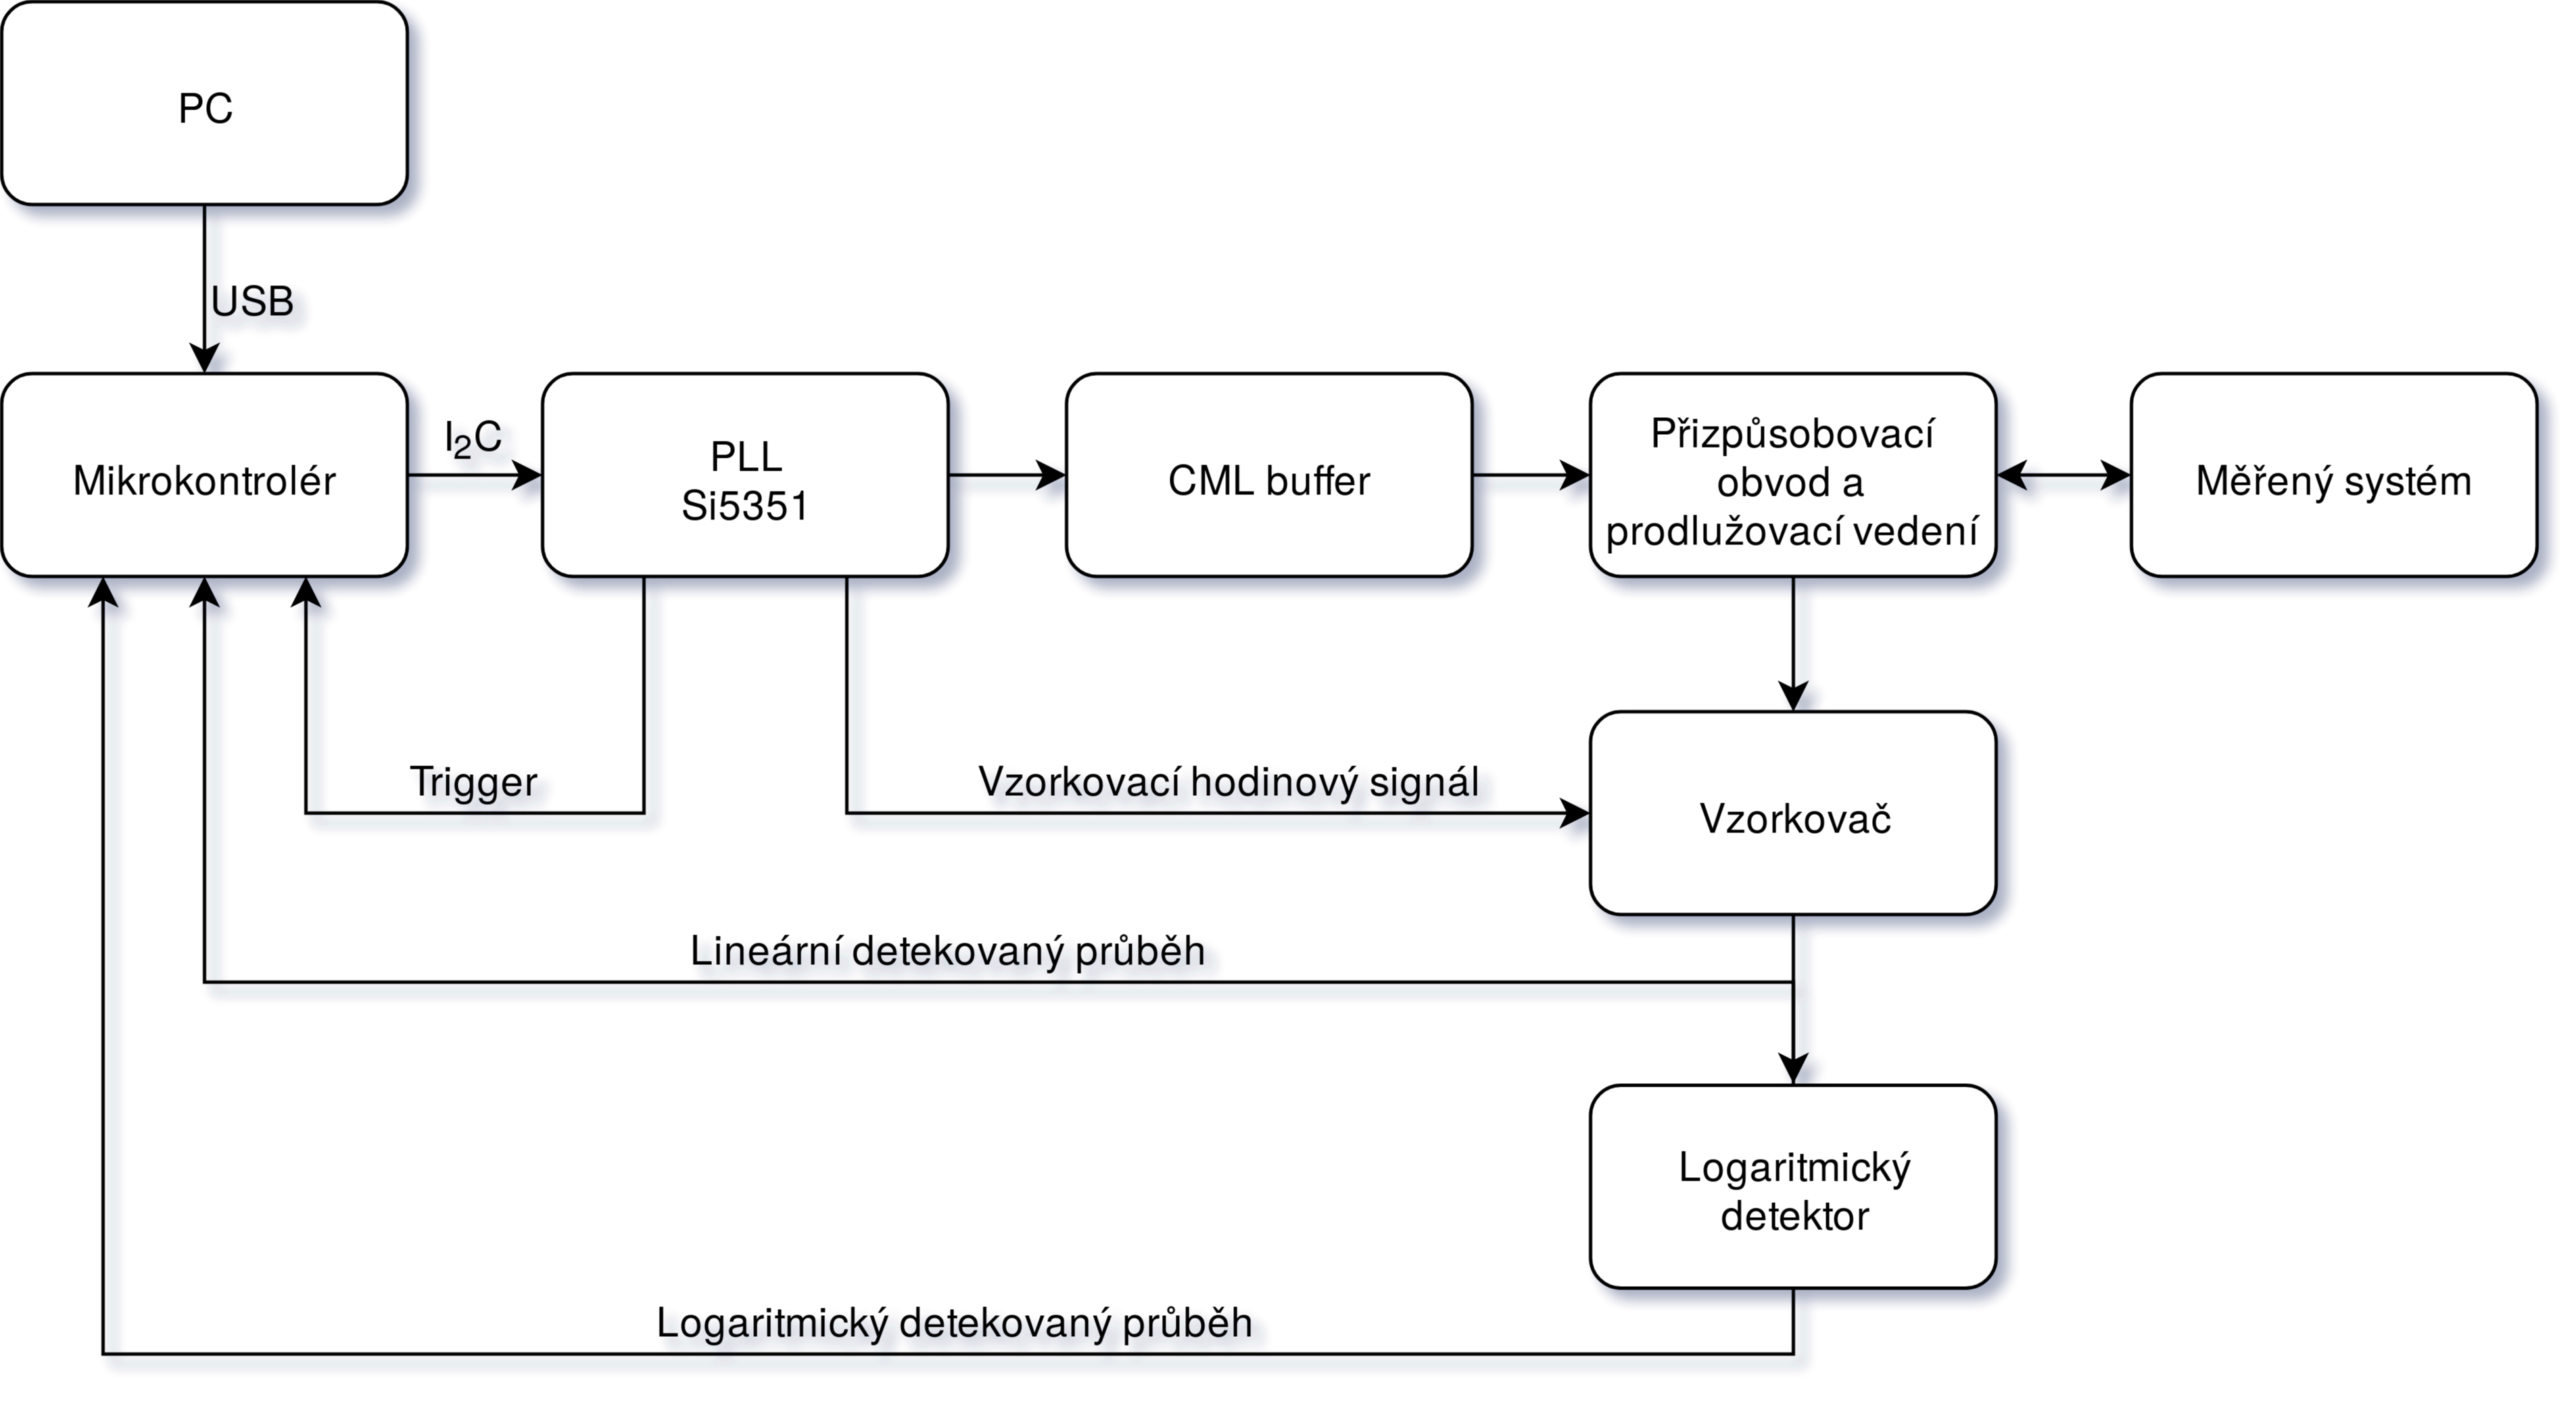
\includegraphics[width=\textwidth,keepaspectratio]{images/reflectometer_blockdiagram_simple.png}\caption{Základní blokové schéma navržené architektury reflektometru.}\label{reflectometer_blockdiagram}\end{figure}
%\chapter{Princip měření}

\section{Základní princip měření}
Reflektometrie v časové oblasti (dále již jen reflektometrie) v kontextu této práce znamená měření vlastností jednobranu, které probíhá na základě měření odezvy měřeného systému na budicí signál, přičemž toto měření probíhá v časové oblasti. Pro měření je možné použít jako budicí signál libovolný kauzální signál, typicky se však využívají pouze průběhy podobné pravoúhlému průběhu nebo jednotkovému v případě širokopásmových reflektometrů. Vzhledem k tomu, že není možné je fyzicky realizovat, protože by vyžadovaly nekonečnou šířku pásma generátoru pulzů, používají se podobné signály, například chybová funkce \cite{S-4manual} nebo Gaussův pulz \cite{ultrawidebandsignals}. V případě úzkopásmových reflektometrů se používá například sinusový průběh modulovaný Gaussovým pulzem \cite{sincgausstdr}. Pro diagnostiku vedení, která jsou v době měření používána pro komunikaci, se používá například pseudonáhodný průběh \cite{noisedomainreflectometry}.

Za předpokladu lineárního invariantního systému a kauzálního budicího signálu je možné závislost odezvy měřeného systému na budicím signálu zapsat následujícím způsobem \cite{principlesoflinearsystems}, kde $x(t)$ je budicí signál, $y(t)$ je změřená odezva systému na daný budicí signál a $h(t)$ je impulzní odezva:
\begin{equation}
y(t)=x(t) \ast h(t).
\end{equation}

Při měření reflektometrem je cílem získat tuto impulzní odezvu, případně skokovou odezvu. Tu je možné buď přímo použít k hrubé analýze měřeného systému nebo provést kalibrační měření, kterým je možné odstranit některé chyby měření, a měřený systém analyzovat výrazně přesněji. Na digitální reflektometry je možné ve frekvenční oblasti aplikovat podobné korekční algoritmy, jako na vektorové analyzátory.

V případě odstranění systémových chyb měření je možné provádět složitější analýzy měřeného systému, např. vypočítat impedanční profil měřeného vedení nebo použít reflektometr podobně jako jednoportový vektorový analyzátor.

\section{Měření v ekvivalentním čase}
Pro vysokorychlostní měření se používají dvě metody měření, měření v reálném čase a měření v ekvivalentním čase.

Měření v reálném čase zpravidla probíhá tak, že jsou všechna měřená data získána z jediné realizace měřeného průběhu. Toto měření je spuštěno předem definovanou spouštěcí událostí, načež je velice rychle změřeno velké množství vzorků. Výhodou tohoto typu měření je možnost změřit jednorázové jevy. Nevýhodou je omezený vzorkovací kmitočet, který se v současné době pohybuje v jednotkách \si{\gigasample}. Dále je nevýhodou nezbytnost velice rychle zpracovávat velké množství dat. Tato metoda měření vyžaduje využití velice rychlých digitálních obvodů. Dodnes se v reflektometrech běžně nevyužívá, neboť neumožňuje dostatečně vysoké vzorkovací kmitočty.

Měření v ekvivalentním čase naopak probíhá během většího množství realizací měřeného průběhu. Měření probíhá tak, že po každé spouštěcí události je odebrán určitý počet vzorků. Při další spouštěcí události dojde ke zhuštění naměřených dat. Ke změření celého průběhu je nezbytné, aby se měření opakovalo, dokud nejsou změřeny všechny body. Nevýhodou tohoto postupu je pomalejší měření a nemožnost změřit jednorázové jevy, nicméně pro statické úlohy, které jsou pro reflektometrická měření typická, je tato metoda vhodná. Tato metoda měření je téměř nezávislá na skutečném vzorkovacím kmitočtu, který pouze omezuje rychlost měření. Vzorkovací kmitočet je omezen pouze konstrukcí časovacích obvodů. Definuje se pak tzv. ekvivalentní vzorkovací kmitočet, který odpovídá převrácené hodnotě nejkratšího měřitelného časového kroku.

\section{Interpretace měřených výsledků}
Po změření odezvy systému na budicí pulz je výsledkem odezva, která je však zatížená chybami měření. Pro jejich odstranění je možné využít převedení změřeného průběhu do časové domény anásledně aplikaci korekčních algoritmů používaných typicky pro vektorové analyzátory. Je tak možné odstranit přeslechy, útlum vedení připojeného k reflektormetru, odrazy na připojovacích konektorech a frekvenční charakteristiku samotného budicího pulzu.
Po odstranění těchto systémových chyb je možné převést je zpět do časové oblasti. Výsledkem je zkalibrovaný průběh, ze kterého je již možné spočítat např. impedanční profil měřeného systému.




\chapter{Princip zapojení}

\section{Základní princip zapojení}
Zapojení se skládá z generátoru impulsů, vzorkovacích obvodů a řídicího fázového závěsu, který tyto dvě části synchronizuje. Generátor impulzů se používá pro tvorbu budicího signálu, který je zaveden do měřeného systému. Pomocí vzorkovacího můstku se pak provádí měření odezvy měřeného systému. Fázový závěs časuje spouštění generátoru a vzorkovače asynchronně tak, aby se postupně spouštěcí událost obou části vzájemně posouvala. Tím dochází k tomu, že každý vzorek odpovídá jinému bodu měřené odezvy. Zařízení tedy pracuje v režimu měření v ekvivalentním čase. To znamená, že měřená odezva není změřena v reálném čase, ale je pomalu sbírána. V navrženém zapojení dojde při každé periodě budicího signálu ke změření jednoho vzorku odezvy systému.

\section{Blokové zapojení}
\begin{figure}[htbp]
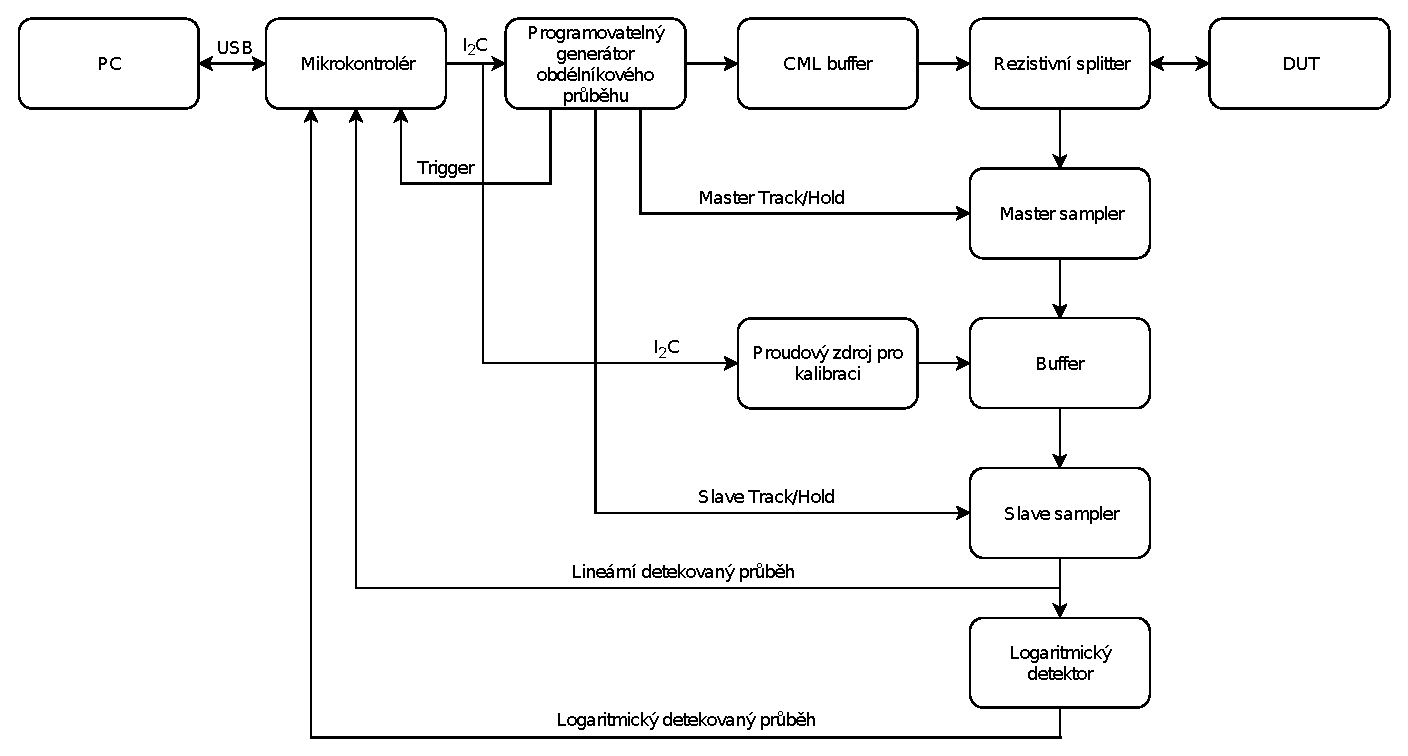
\includegraphics[width=\textwidth,keepaspectratio]{images/block_diagram.eps}\caption{Blokové zapojení reflektometru.} \label{block_diagram}
\end{figure}

Blokové zapojení reflektometru je znázorněno na obrázku \ref{block_diagram}. V dalších částech této kapitoly jsou jenotlivé bloky popsány do hloubky.

\section{Generování potřebných hodinových signálů}
Hlavním prvkem celého zapojení je vícekanálový digitální fázový závěs, který je postaven na obvodu Si5351C-B \cite{Si5351datasheet}. Tento obvod obsahuje krystalový oscilátor, na nějž jsou zavěšeny dva interní oscilátory \acrshort{VCO}. Vnitřní blokové schéma je možné vidět na obrázku \ref{si5351_internal_architecture_overview}.

\begin{figure}[htbp]
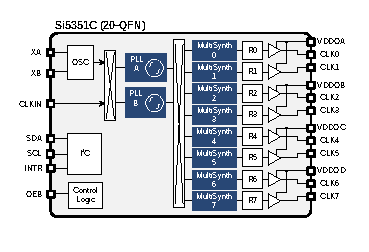
\includegraphics[width=\textwidth,keepaspectratio]{images/si5351_internal_architecture_overview.eps}\caption{Vnitřní blokové zapojení obvodu Si5351, převzato z \cite{Si5351datasheet}.} \label{si5351_internal_architecture_overview}
\end{figure}

Frekvenci těchto oscilátorů je možné nezávisle nastavit. Jejich frekvence $f_{VCO}$ může být neceločíselným násobkem frekvence krystalového oscilátoru $f_{XTAL}$.
\begin{equation}
f_{VCO}=f_{XTAL} \left(a+\dfrac{b}{c} \right)
\end{equation}
Koeficient $a$ může nabývat hodnot $\langle 15, 90 \rangle$. V neceločíselném režimu může koeficient $c$ nabývat hodnot $\langle 0, 1048575 \rangle$, koeficient $b$ pak $\langle 0, c \rangle$.
Je tedy možné nastavit frekvenci oscilátorů tak, že se liší o méně než 1 ppm. Při použití těchto dvou frekvencí jako časovacích signálů pro buzení a vzorkování je tedy možné odebírat až 1048576 vzorků. Dochází totiž k tomu, že s každou periodou se postupně hrany těchto obdélníkových signálů vůči sobě časově posunou o fixní časový krok. Tento krok je možné spočítat z nastavených frekvencí oscilátorů.

\begin{equation}
\begin{gathered}
f_{VCO1}=f_{XTAL} \left(a_1+\dfrac{b_1}{c_1} \right) \\
f_{VCO2}=f_{XTAL} \left(a_2+\dfrac{b_2}{c_2} \right)
\end{gathered}
\end{equation}

Za těmito oscilátory ještě následují děličky. Ty také umožňují neceločíselné dělení, které je ovšem nevýhodné, protože může zvyšovat fázové chvění výstupního signálu. Proto jsou použity pouze v celočíselném režimu. Děličky jsou použity kvůli omezenému vzorkovacímu kmitočtu použitého \acrshort{ADC}. Výsledkem jsou tedy dvě frekvence $f_{OUT1}$ a $f_{OUT2}$. Označíme-li společný dělicí poměr $d$ a za předpokladu, že $a_1=a_2=a$, $c_1=c_2=c$ a $b_2=0$:

\begin{equation}
\begin{gathered}
f_{OUT1}=\dfrac{f_{VCO1}}{d}=f_{XTAL} \left(\dfrac{a+\dfrac{b_1}{c} }{d}\right) \\
f_{OUT2}=\dfrac{f_{VCO2}}{d}=f_{XTAL} \left(\dfrac{a}{d}\right)
\end{gathered}
\end{equation}

Pak se během jedné periody oscilátory vůči sobě posunou o čas $T_{SHIFT}$:

\begin{equation}
\begin{gathered}
T_{SHIFT}=T_{OUT2}-T_{OUT1}=\dfrac{1}{f_{OUT2}} - \dfrac{1}{f_{OUT1}} \\
T_{SHIFT}=\dfrac{d}{f_{XTAL}} \left(\dfrac{1}{a} - \dfrac{1}{a+\dfrac{b_1}{c}}\right) = \dfrac{d}{a f_{XTAL}} \left(\dfrac{1}{1+a\dfrac{c}{b_1}}\right)
\end{gathered}
\end{equation}

Pro minimalizaci fázového chvění je podle \cite{Si5351datasheet} a \cite{Si5351applicationnote} vhodné preferovat celočíselné násobení i dělení, je-li to možné. Dále může fázové chvění zmenšit i použití sudých násobitelů a dělitelů. V navrženém zapojení je tedy fázový závěs nastaven takto:

\begin{equation}
\begin{gathered}
f_{XTAL}=\SI{25}{MHz} \\
a=24 \;\;\; b_1=24/8=3 \\
c=500000/8=62500 \;\;\; d=128 \cdot 46=5888 \\
f_{OUT1} \doteq \SI{101902}{kHz} \doteq f_{OUT2} \\
T_{SHIFT} = \dfrac{46 \cdot 128}{24 \cdot 25000000} \left(\dfrac{1}{1+24 \cdot \dfrac{500000}{24}}\right) \doteq \SI{19.627}{ps}
\end{gathered}
\end{equation}

Podobný princip měření pomocí dvou oscilátorů o podobné frekvenci se již v literatuře objevil, avšak zatím nebyl implementován přímo pomocí fázového závěsu. V \cite{vernierreflectometer} byly použity dva nezávislé oscilátory. Toto řešení je sice jednodušší, avšak není možné zajistit, jak velký bude časový krok měření. Vzhledem ke skutečnosti, že oscilátory jsou závislé na teplotě a dalších vnějších vlivech, není možné zajistit ani dlouhodobou stabilitu. Při použití dvojitého fázového závěsu s neceločíselným násobitelem však je možné tuto dlouhodobou stabilitu zajistit. Krok měření je pak závislý pouze na frekvenci jediného krystalového oscilátoru. Při použití \acrshort{TCXO} může být tato stabilita velmi dobrá, na úrovni jednotek \si{ppm}.

Další podobný způsob časování vzorkování je použit v \cite{ddsfpgareflectometer}, kde je využito \acrshort{FPGA} jako \acrshort{DDS}. Výstup z této \acrshort{DDS} je filtrován dolní propustí a následně zaveden do komparátoru, římž je získáván obdélníkový řídicí signál. Řízení vzájemné polohy budicího pulzu a vzorkování je pak dosaženo nastavováním fáze sinusového signálu, který je generován \acrshort{DDS}. Tento systém umožňuje krok vzorkování v jednotkách pikosekund. Je tedy podobný vlastnostmi konstrukci popsané v této práci. Něvýhodou je však to, že autoři se příliš nezabývali generátorem impulzů, náběžná hrana použitého generátoru činí přibližně \SI{2}{ns}. Důvod, proč tak autoři učinili, je možná omezení vyplývající ze zvoleného způsobu vzorkování pomocí komparátoru a digitálního integrátoru.

\begin{figure}[htbp]
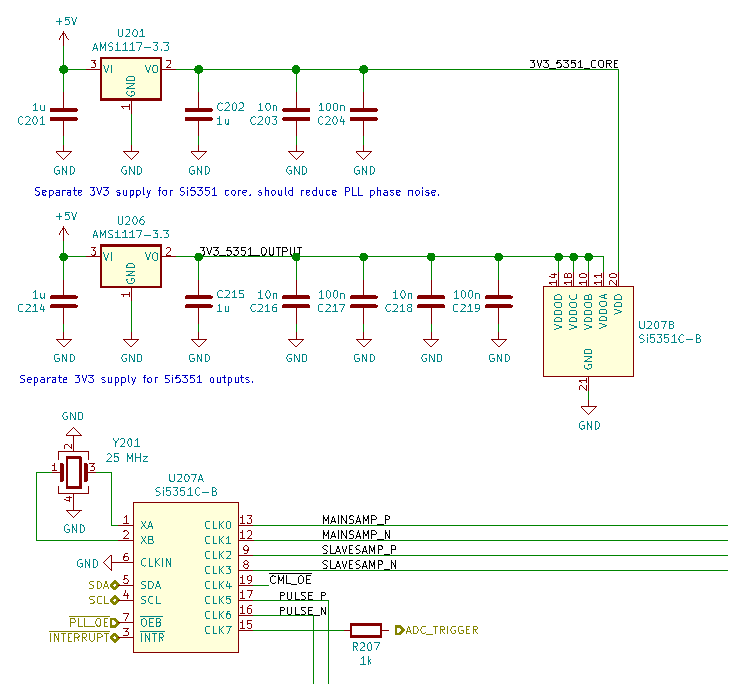
\includegraphics[width=\textwidth,keepaspectratio]{images/timing_section.eps}\caption{Zapojení hodinového generátoru Si5351.}\label{timing_section_schematic}
\end{figure}	

Zapojení hodinového generátoru s fázovým závěsem Si5351 je zobrazeno na \ref{timing_section_schematic}. Symbol obvodu je rozdělený na dvě části, U207A a U207B. Kromě samotného obvodu Si5351 je potřeba pouze referenční krystal a napájecí obvody. Napájení je rozděleno na dvě domény. První je jádro fázového závěsu, které napájí interní logické obvody a \acrshort{VCO}. Druhá napájí výstupní budiče. Toto rozdělení by mělo omezit fázový šum generovaných hodinových signálů způsobený rušením na napájení \acrshort{VCO} \cite{Si5351applicationnote}. Pro krystalový oscilátor není potřeba používat zatěžovací kondenzátory, jsou obsaženy uvnitř obvodu Si5351, je možné je nastavit v rozsahu \SIrange{4}{10}{\pico\farad}.

Výstupní budiče obvodu Si5351 jsou slučitelné jak s \acrshort{CMOS} obvody a jejich modernějšími variantami, tak i s obvody rodin \acrshort{TTL}, \acrshort{ECL}, \acrshort{CML}, \acrshort{LVDS} a podobnými. Budiče jsou proudové, proud je možné nastavit ve čtyřech krocích v rozsahu \SIrange{2}{8}{\milli\ampere} \cite{Si5351datasheet}. Tohoto faktu je využito v zapojení, 4 výstupy jsou použity přímo pro proudové buzení vzorkovacích můstků, 2 výstupy pro buzení \acrshort{CML} bufferu, jeden výstup pro synchronizaci vzorkování použitého mikrokontroléru a jeden výstup pro řízení stavu \acrshort{CML} bufferu.

Dle katalogových údajů by tento fázový závěs měl typicky dosahovat mezivrcholového fázového šumu \SI{70}{\pico\second}, maximálně  \SI{155}{\pico\second}. Dle výrobce by mělo jít o parametry v \quotedblbase nejhorším možném případě v reálné aplikaci \ldots{} skutečné vlastnosti mohou být výrazně lepší\textquotedblleft{} \cite{Si5351datasheet}. Bohužel není uvedeno, jak se tento parametr mění v závislosti na nastavení násobicích a dělicích sekcí. Není uveden ani histogram šumu, jeho frekvenční spektrum, ani efektivní hodnota. Spektrum fázového šumu je možné najít v \cite{Si5351_phase_noise_measurement}, bohužel se nejedná o ověřený zdroj.

\section{Tvorba budicího pulzu}
Pro tvorbu budicích pulzů byl vybrán obvod SY54020, který je původně určen jako \acrshort{CML} buffer. Logické obvody \acrshort{CML} používají logické úrovně referencované vůči kladnému pólu napájení, výstupy i vstupy těchto obvodů jsou přizpůsobené impedanci \SI{50}{\ohm}. Podle katalogových údajů \cite{SY54020datasheet} by měla výstupní impedance ležet v rozsahu \SIrange{45}{55}{\ohm}. Hlavní důvod pro použití tohoto bufferu je vysoká rychlost, dle katalogových údajů by měla délka náběžných a sestupných hran spadat do rozsahu \SIrange{35}{100}{\pico\second}, typicky \SI{60}{ps}. Tento údaj je udáván pro body, kde prochází náběžná hrana \SI{20}{\%} a \SI{80}{\%} mezi původním a konečným napětím. U obvodu Si5351 by podle katalogových údajů měl tento parametr být typicky \SI{1}{\nano\second}, maximálně \SI{1.5}{\nano\second}. Použitím obvodu SY54020 by tedy mělo být možné zkrátit náběžné hrany o \SIrange{90}{98}{\%} oproti přímému použití výstupu z obvodu Si5351 jako zdroje budicích pulzů. Dle katalogových údajů by špičkový aditivný fázové chvění mělo být přibližně \SI{1}{\pico\second}, tedy přibližně o dva řády lepší, než fázové chvění obvodu Si5351. Použití budiče SY54020 by tedy mělo mít zcela minimální vliv na celkovou úroveň fázového chvění.

\begin{figure}[htbp]
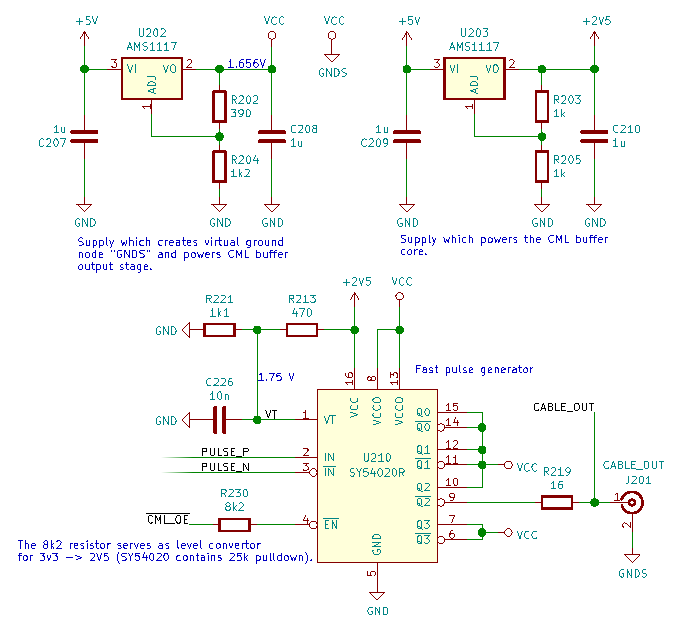
\includegraphics[width=\textwidth,keepaspectratio]{images/pulse_generator_section.eps}\caption{Zapojení generátoru budicích pulzů}\label{pulse_generator_section_schematic}
\end{figure}	

Postatná výhoda obvodu SY54020 spočívá v oddělení napájecích úrovní vstupů a výstupů tohoto obvodu. V zapojení je vstupní část obvodu napájena \SI{3.3}{\volt}, výstupní část \SI{1.65}{\volt}, tedy přesně polovičním napájecím napětím. Tato napájecí hladina označená jako VCC, a zároveň jako GNDS, je použita jako virtuální analogová země. Všechny následující obvody jsou vztažené k této virtuální zemi. Zapojení generátoru budicích impulzů je na obrázku \ref{pulse_generator_section_schematic}.

\section{Přizpůsobovací obvody a testovací port}
Generátor budicích impulzů z předchozího bodu je nezbytné připojit k měřicímu portu. K tomuto portu však musí být zároveň připojeny vzorkovací obvody. Proto jsou nezbytné přizpůsobovací obvody, které umožňují připojit k testovacímu portu obě tyto části při dodržení vstupní impedance. Jejich zapojení je uvedeno na obrázku \ref{match_section_schematic}.

\begin{figure}[htbp]
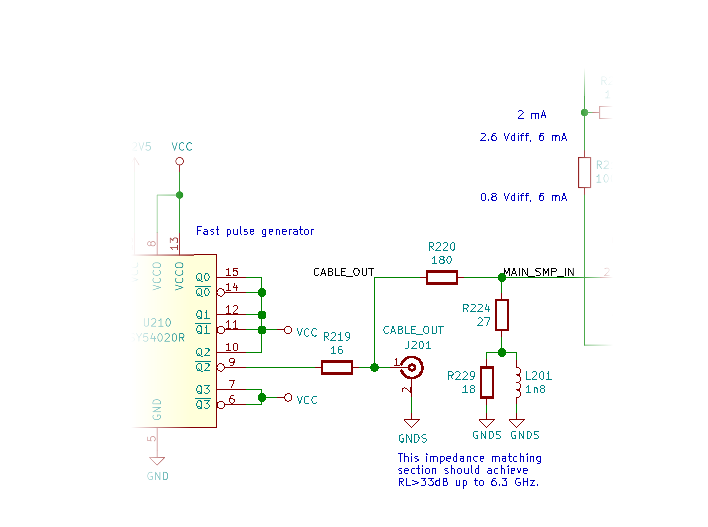
\includegraphics[width=\textwidth,keepaspectratio]{images/match_section.eps}\caption{Schéma přizpůsobovacích obvodů.}\label{match_section_schematic}
\end{figure}

Přizpůsobovací obvody jsou navrženy tak, aby bylo dosaženo co nejlepšího impedančního přizpůsobení na testovacím konektoru. Problematická je impedance vzorkovacího můstku, neboť na jeho výstupu je připojen vzorkovací kondenzátor, který způsobuje rezonanci pouzdra vzorkovacího můstku na frekvenci přibližně \SI{1.7}{\giga\hertz}. Vliv této rezonance na vstupní impedanci reflektometru je částečně potlačen použitím děliče sestaveného z odporů R220, R224 a R229 a cívky L201 (označení podle obrázku \ref{match_section_schematic}). Výsledná impedance je zakreslena v grafu \ref{input_impedance}, parametr $S_{11}$ pak v grafu \ref{input_reflection}. Simulace byla provedena bez vední T1, které se nachází na schématu \ref{ltspice_schematic}. Hodnoty použitých součástek v děliči se mezi schématy liší, protože během vývoje zařízení byly použité diodové můstky HSMS-282P vyřazeny z výroby. Jako náhrada byly vybrány diodové můstky SMS3923-081LF. Díky podrobnějšímu SPICE modelu bylo možné do simulace zahrnout i vliv parazitních vlastností pouzdra tohoto můstku, což umožnilo další optimalizace. Konečné hodnoty použitých součástek se nachází ve schématu použitém v simulaci.

\begin{figure}[htbp]
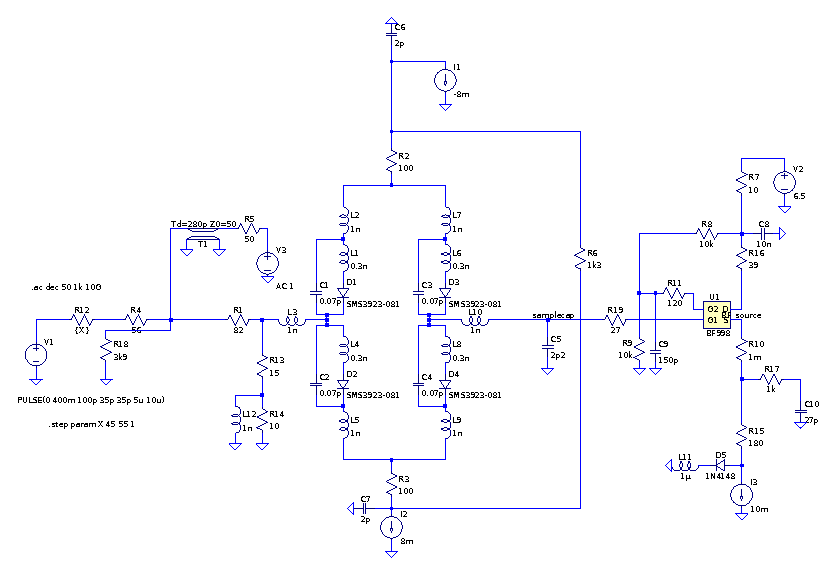
\includegraphics[width=\textwidth,keepaspectratio]{images/ltspice_schematic.eps}\caption{Schéma použité pro simulaci vstupní impedance v programu LTSpice.}\label{ltspice_schematic}
\end{figure}

\begin{figure}[htbp]
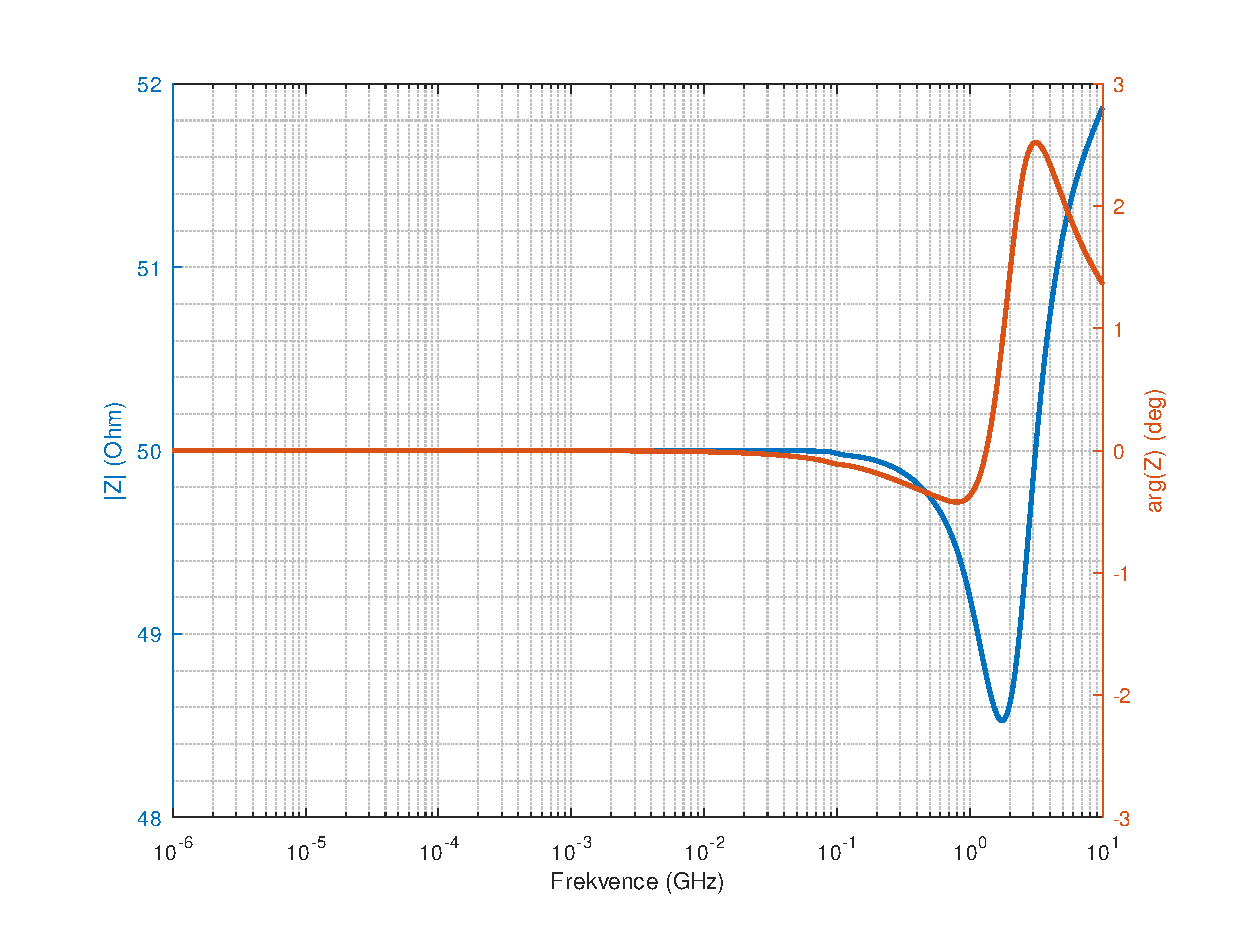
\includegraphics[width=\textwidth,keepaspectratio]{images/input_impedance.eps}\caption{Vstupní impedance reflektometru.}\label{input_impedance}
\end{figure}

\begin{figure}[htbp]
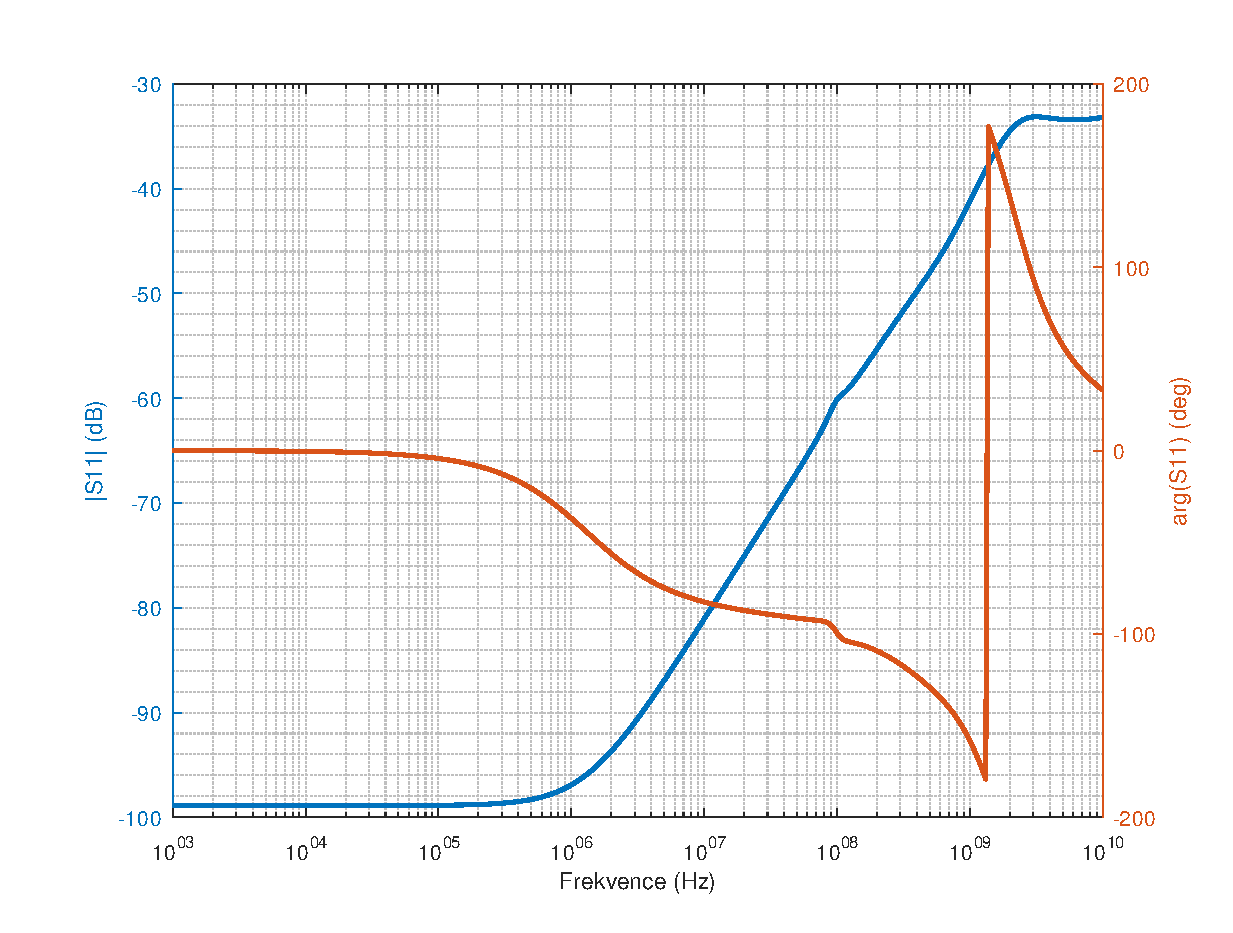
\includegraphics[width=\textwidth,keepaspectratio]{images/input_reflection.eps}\caption{Přizpůsobení vstupní impedance reflektometru.}\label{input_reflection}
\end{figure}

Vstupní impedance byla simulována do 10 GHz. V celém simulovaném pásmu se vstupní impedance odchyluje od nominálních $50~\Omega$ o méně než $\pm2~\Omega$. Parametr $\lvert S_{11} \rvert$ je vykreslen v grafu \ref{input_reflection}. V celém rozsahu je menší než \SI{-33}{\deci\bel}, což odpovídá koeficientu odrazu $\Gamma <= 0.023$. Navržené přizpůsobení by tedy mělo být velmi dobré. Vzhledem k tomu, že konektory obvykle způsobují odraz větší, než je odraz vycházející ze simulace, měl by být klíčovým prvkem pro dosažení malého odrazu na testovacím portu kvalitní konektor a připojovací vedení. Při uvažování tolerance impedance budiče SY54020, která se pohybuje v rozsahu \SIrange{45}{55}{\ohm}, se přizpůsobení zhorší, nicméně v celém rozsahu je lepší než \SI{-30}{\deci\bel}.

\section{Vzorkovací obvody a oddělovací zesilovač}
Vzorkování je v reflektometru prováděno ve třech stupních. První stupeň je tvořený diodovým můstkem U208 (na obrázku \ref{sampler_section_schematic}) a kondenzátorem C230. Druhý stupeň vzorkování je tvořen diodovým můstkem U209 a kondenzátorem C233. Třetí stupeň probíhá uvnitř mikrokontroléru v \acrshort{ADC}.

První vzorkovací stupeň je připojen k obvodu Si5351, který proudově napájí vzorkovací můstek. Proud nastavený na budičích tohoto obvodu je \SI{8}{\milli\ampere}. V době, kdy vzorkovač sleduje vstupní signál, jsou diody sepnuty v propustné oblasti, můstek se pak chová přibližně jako rezistor o odporu jednotek \si{\ohm} zapojený mezi vstupem a vzorkovacím kondenzátorem. V okamžiku, kdy má být odebrán vzorek měřeného napětí, se obrátí směr proudu tekoucí skrz můstek, čímž se můstek rozepne. Po rozepnutí má můstek charakter kondenzátoru o kapacitě desetin pikofaradu. Aby můstek co nejméně ovlivňoval vstupní impedanci reflektometru, je připojen přes přizpůsobovací obvody. Kondenzátor C230 musí mít co nejmenší kapacitu, aby příliš kapacitně nezatěžoval vzorkovací můstek. Při použití většího kondenzátoru klesá šířka propustného pásma vzorkovače a zvětšuje se vliv vzorkovače na vstupní impedanci reflektometru. Pro potlačení kapacitního charakteru vzorkovače je v přizpůsobovacím obvodu použita kombinace R229 a L201, které částečně na vysokých frekvencích stáčí impedanci zpět k reálným hodnotám. Při použití příliš malého kondenzátoru je problematická parazitní kapacita diodového můstku v rozepnutém stavu, měřený signál pak výrazně \quotedblbase prosakuje\textquotedblleft{} do navzorkovaného signálu i v okamžiku, kdy je diodový můstek rozepnutý.

\begin{figure}[htbp]
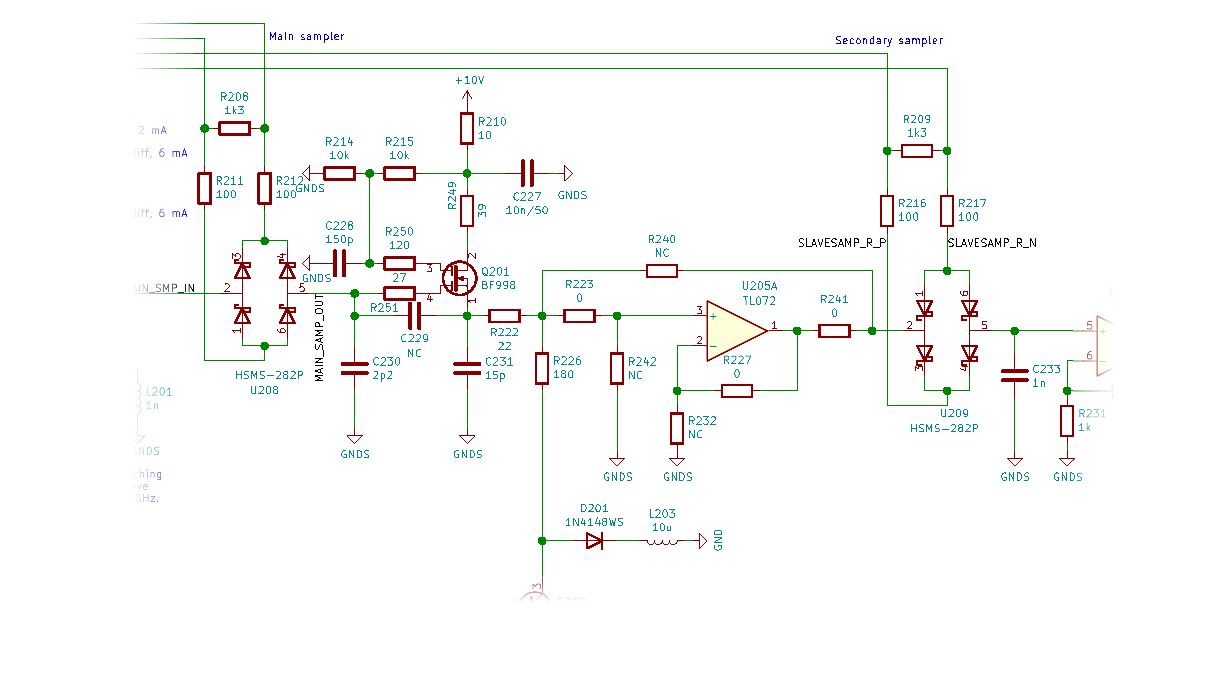
\includegraphics[width=\textwidth,keepaspectratio]{images/sampler_section.eps}\caption{Zapojení vzorkovacích obvodů.}\label{sampler_section_schematic}
\end{figure}

Vzhledem k velice malé kapacitě vzorkovacího kondenzátoru je nezbytné, aby obvody připojené k němu měly minimální vstupní proud. To by bylo možné zajistit přímo unipolárním operačním zesilovačem U205, avšak má velkou vstupní kapacitu, přibližně 27 pF \cite{oscilloscopefrontend}. Proto je použit oddělovací zesilovač s unipolárním dvouhradlovým tranzistorem BF998 s malou kapacitou hradla. Vstupní impedance oddělovacího zesilovače je přibližně do \SI{900}{\mega\hertz} takřka čistě imaginární, kapacita odpovídající této impedanci je přibližně \SI{0.6}{\pico\farad} na \SI{10}{\mega\hertz} a \SI{0.9}{\pico\farad} na \SI{1}{\giga\hertz}. Zesilovač je zapojen jako sledovač signálu s jednotkovým ziskem. V source tranzistoru je zapojen proudový zdroj kvůli minimalizaci zkreslení. Dle simulace by stejnosměrné zkreslení zesilovače mělo být lepší než \SI{0.0005}{\%}, absolutní chyba výstupního napětí je uvedena v grafu \ref{buffer_voltage_error}. Rozkmit měřeného napětí je podle simulací \SI{20}{\milli\volt}.

Při návrhu zapojení byly uvažovány i varianty s jinými tranzistory. Bohužel nebyl nalezen žádný tranzistor, který by byl  schopen pracovat do vyšších frekvencí a přitom měl nízký vstupní proudl hradla. Moderní tranzistory HEMT bohužel zpravidla mají vstupní proud v řádu mikroampérů. Rychlejší tranzistory typů MOSFET nebo MESFET se vyrábí pouze pro výkonové aplikace. Ke vhodným tranzistorům typu JFET se bohužel dodávají pouze S-parametry a nejsou dostupné parametry pro SPICE modely. Nakonec tedy byl zvolen tranzistor BF998. 

Maximální hodnotu kapacity kondenzátoru C230 určuje i oddělovací zesilovač. Při kapacitě větší než \SI{1.5}{\pico\farad} by se oddělovací zesilovač rozkmital, což bylo zjištěno v zapojení během testování. Následně byla tato skutečnost potvrzena simulací a opravena. Proto jsou v zesilovači použity odpory R249, R250 a R251. R251 omezuje kladnou zpětnou vazbu a tlumí rezonanci páru U208~--~C230, čímž je zabráněno rozkmitání zesilovače. Odpor R249 nadále zeslabuje tuto kladnou zpětnou vazbu. Odpor R250 zvětšuje vstupní impedanci zesilovače a zvětšuje šířku pásma tohoto oddělovacího stupně. Kondenzátor C231 není v konečném zapojení použit, neboť zmenšoval použitelnou šířku pásma zesilovače a zhoršoval stabilitu zapojení. Přenosová charakteristika oddělovacího zesilovače je uvedena v grafu \ref{frequency_transfer_function_bf}.Podle těchto odsimulovaných výsledků by měla být 6\si{\deci\bel} šířka pásma přibližně \SI{5.9}{\giga\hertz}.

\begin{figure}[htbp]
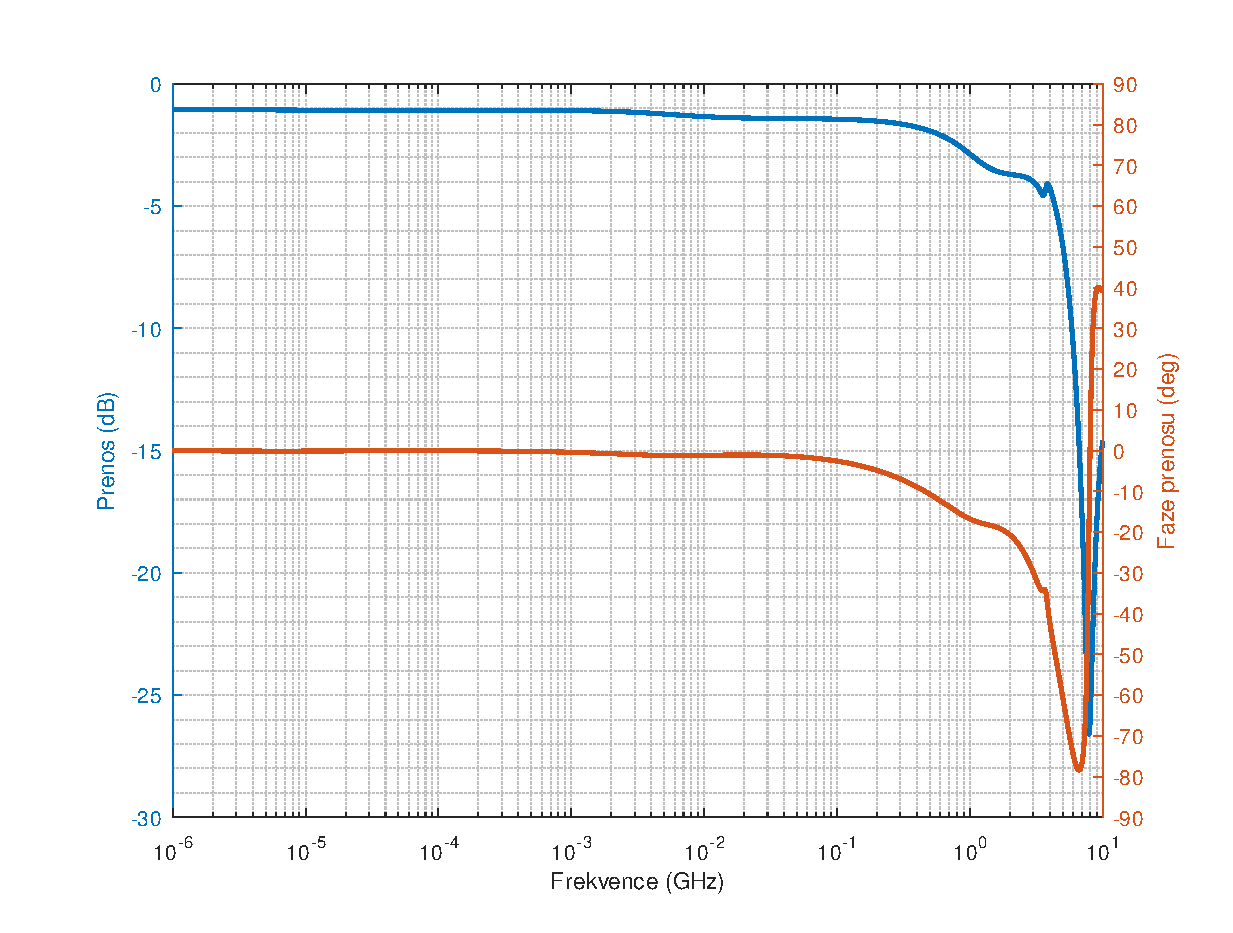
\includegraphics[width=\textwidth,keepaspectratio]{images/frequency_transfer_function_BF.eps}\caption{Přenos oddělovacího zesilovače.}\label{frequency_transfer_function_bf}
\end{figure}

Celková přenosová charakteristika od testovacího portu až k výstupu oddělovacího zesilovače je uvedena v grafu \ref{frequency_transfer_function_all}. 6\si{\deci\bel} šířka pásma pak činí přibližně \SI{1.93}{\giga\hertz}.

\begin{figure}[htbp]
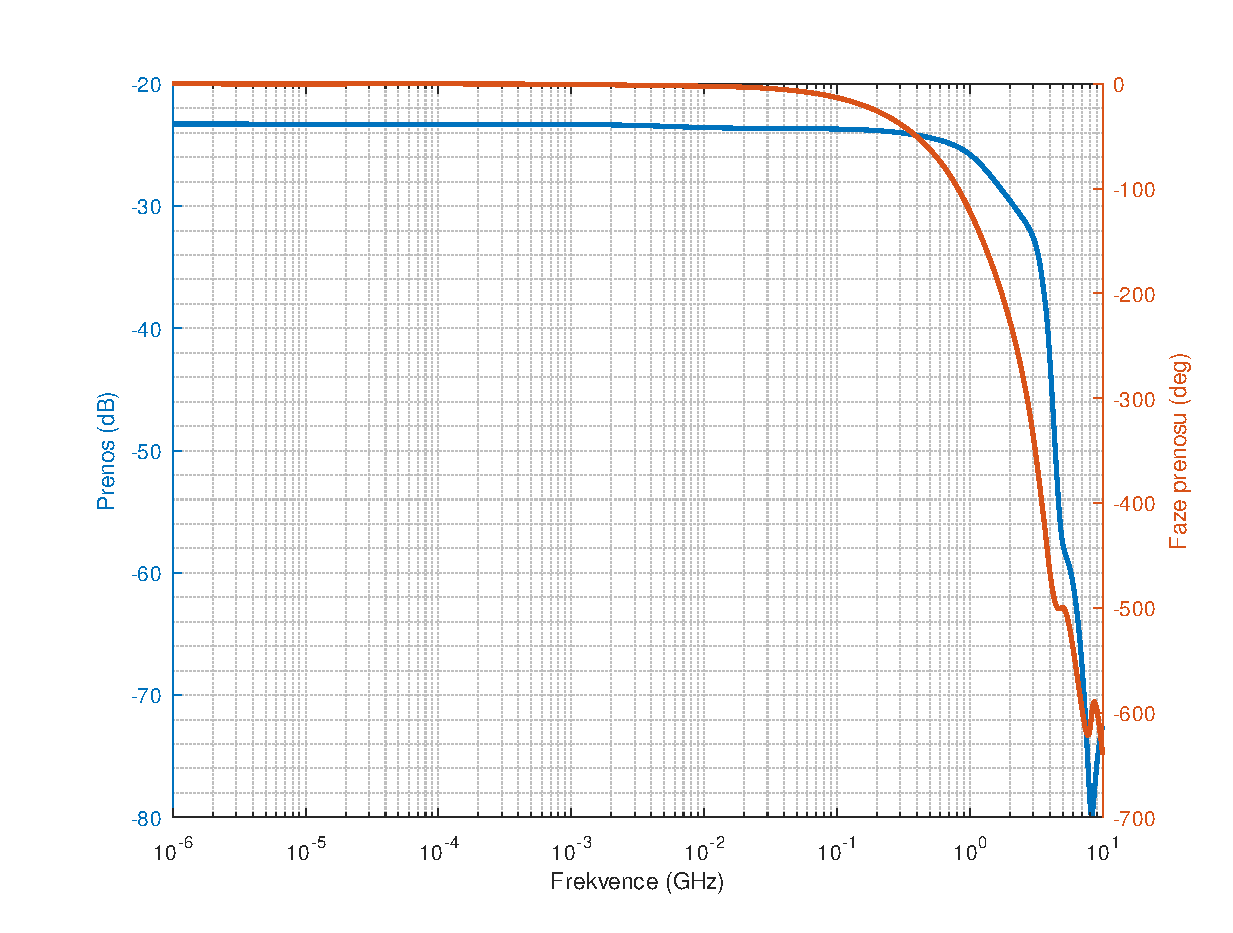
\includegraphics[width=\textwidth,keepaspectratio]{images/frequency_transfer_function_all.eps}\caption{Přenos celého systému přizpůsobení-vzorkovač-zesilovač.}\label{frequency_transfer_function_all}
\end{figure}

Simulace nebyla provedena s idealizovaným proudovým zdrojem, ale již v zapojení, které je uvedeno na schématu \ref{sampler_section_schematic}. Simulovaná data by tak měla lépe odpovídat realitě. Důvod, proč na schématu \ref{ltspice_schematic} není uvedeno celé zapojení proudového zdroje, ale jen idealizovaného zdroje, je časová náročnost výpočtů. Při simulacích vstupní impedance má tato část minimální vliv na výsledky, ale výrazně zpomaluje výpočty, proto byla ze simulací týkajících se vstupní impedance a tranzientních simulací oddělovacího zesilovače vynechána. Celé zapojení proudového zdroje je vidět na schématu \ref{current_source_section_schematic}.

\begin{figure}[htbp]
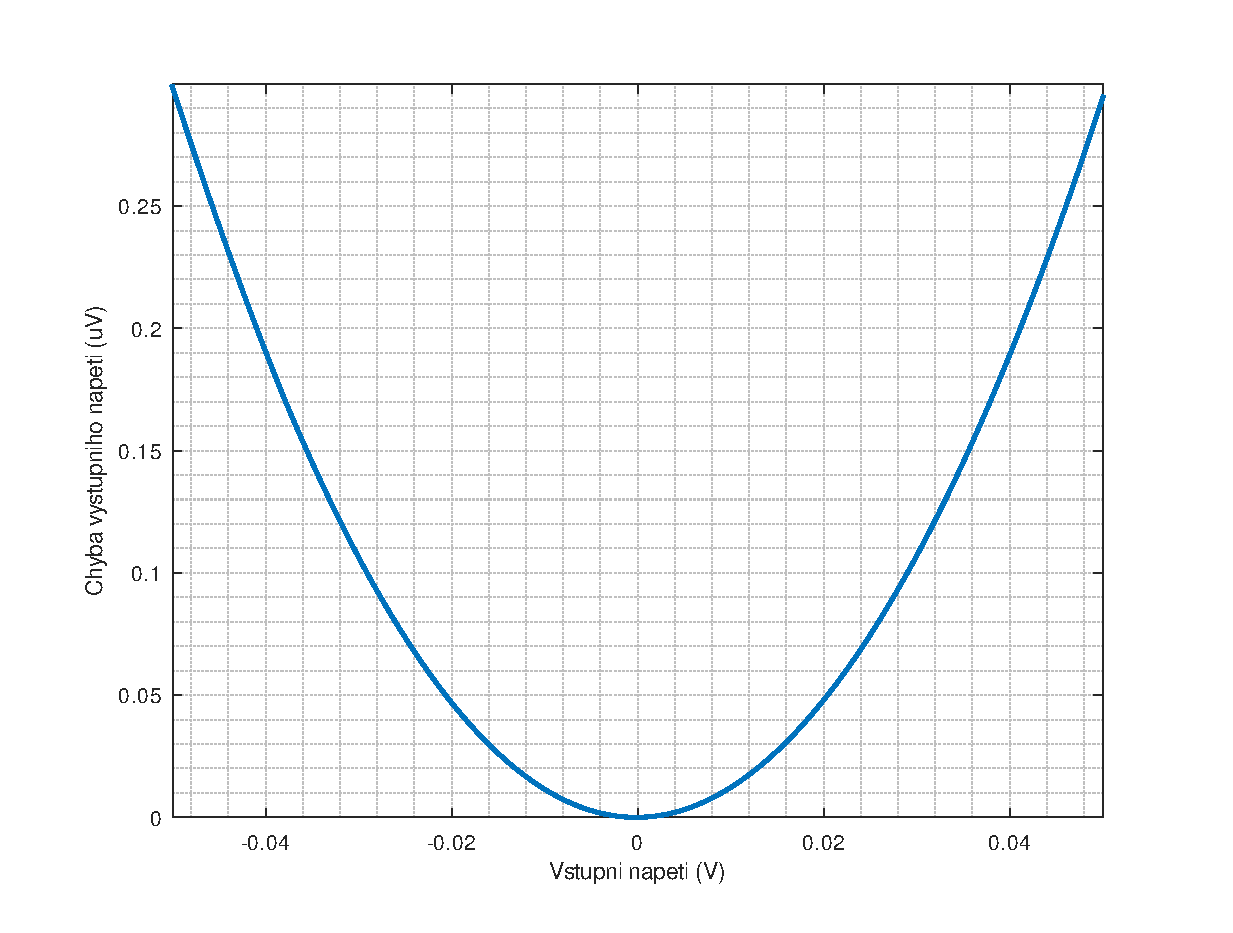
\includegraphics[width=\textwidth,keepaspectratio]{images/transfer_characteristic.eps}\caption{Absolutní chyba linearity oddělovacího zesilovače.}\label{buffer_voltage_error}
\end{figure}

\begin{figure}[htbp]
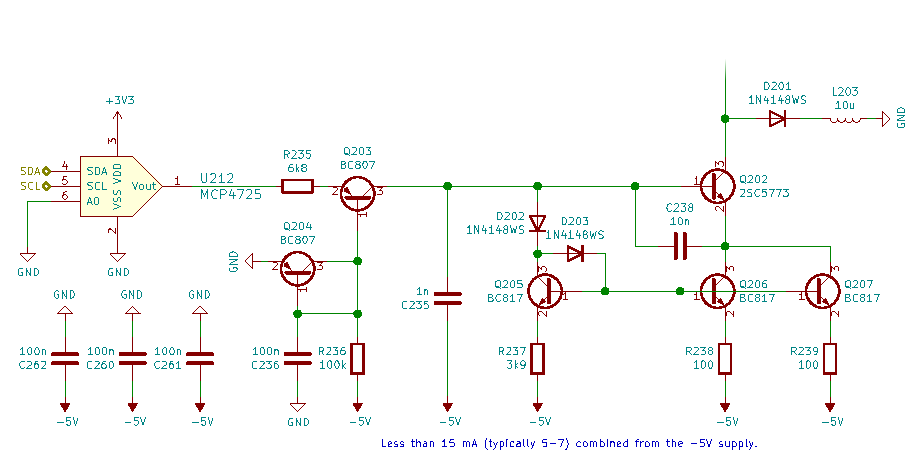
\includegraphics[width=\textwidth,keepaspectratio]{images/current_source_section.eps}\caption{Zapojení proudového zdroje.}\label{current_source_section_schematic}
\end{figure}

Proudový zdroj na schématu \ref{current_source_section_schematic} napájí oddělovací zesilovač. Zdroj je řízen \acrshort{DAC}, je možné jej nastavit v rozsahu \SIrange{0}{15.9}{\si{mA}} v 4096 krocích po přibližně \SI{3.88}{\micro\ampere}. Zroj je určen k autokalibraci reflektometru, umožňuje stejnosměrné posunutí měřeného signálu. Tento autokalibrační proces je nezbytný kvůli výrobním tolerancím a teplotní závislosti unipolárního dvouhradlového tranzistoru BF998. Proudový zdroj je zapojen jako kaskodové proudové zrcadlo. Odpor R235 spolu s tranzistory Q203 a Q204 slouží jako převodník z napětí na proud. Tranzistory Q202, Q205, Q206 a Q207 tvoří proudové zrcadlo. V emitorech tranzistorů jsou zapojeny odpory, čímž se zrcadlo podobá Widlarově proudovému zrcadlu se zesilovacím poměrem přibližně 60. Tranzistor Q202 je vysokofrekvenční typ s $f_T=\SI{6}{\giga\hertz}$ při \SI{8}{\milli\ampere} a nízkou výstupní kapacitou kolektoru, $C_ob<\SI{1.8}{\milli\ampere}$. Pro ochranu tranzistoru Q202 před lavinovým průrazem během zapínání reflektometru a autokalibrace je použita dioda D201, která omezuje napětí kolektor-emitor na tranzistoru Q202 na přibližně \SI{4}{\volt}, průrazné napětí tranzistoru je dle katalogových údajů \SI{6}{\volt}. Proudový zdroj je navržen tak, že není možné nastavit proud emitorem tranzistoru Q202 větší než \SI{15}{\milli\ampere}, přičemž povolený trvalý proud je \SI{50}{\milli\ampere}. Tranzistor by tedy měl být kompletně ochráněn před poškozením. Pro potlačení vlivu kapacity diody D201 na přenos oddělovacího zesilovače na vysokých frekvencích je použita cívka L203.

\begin{figure}[htbp]
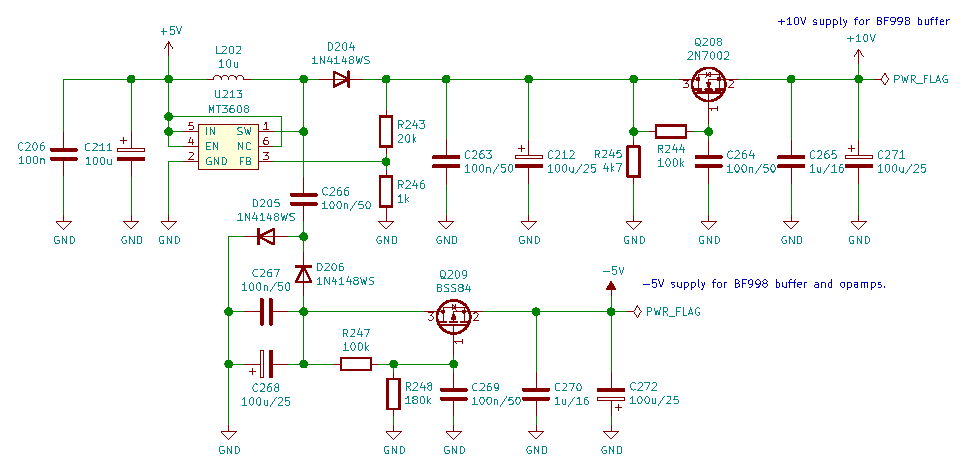
\includegraphics[width=\textwidth,keepaspectratio]{images/power_supply_section.eps}\caption{Zapojení napájecích zdrojů vzorkovacích obvodů.}\label{analog_source_section_schematic}
\end{figure}

Napájecí zdroj operačních zesilovačů, proudového zdroje a oddělovacího zesilovače je na schématu \ref{analog_source_section_schematic}. Zdroj je napájen z \SI{5}{\volt} získávaných z USB. Jádrem je spínaný zdroj MT3608 pracující na frekvenci \SI{2}{\mega\hertz}, který je nastaven na napětí \SI{12.6}{\volt}. Tato napájecí větev je filtrována aktivním filtrem s tranzistorem Q208. Napájecí hladina \SI{12.6}{\volt} je filtrována RC článkem R244-C264. Toto vyfiltrované napětí je zapojeno do gate tranzistoru Q208, který je zapojen jako sledovač. Teoreticky je tak možné zajistit značné potlačení zvlnění napětí na napájecí větvi. Výsledkem je vyfiltrované nestabilizované napětí přibližně \SI{10}{\volt}. Potlačení zvlnění by dle simulace mělo být přibližně \SI{-128}{\deci\bel} na frekvenci \SI{2}{\mega\hertz}, kde pracuje spínaný zdroj. Přenosová charakteristika tohoto aktivního filtru je na grafu \ref{analog_source_filter_transfer}, je vyznačená modře.

Záporná napájecí větev je získávána z téhož zdroje pomocí nábojové pumpy tvořené kondenzátory C266 -- C268 a diodami D205 a D206. Výsledné napětí je přibližně \SI{-12}{\volt}. Tranzistor Q209 opět tvoří aktivní filtr. Odporovým děličem je nastaveno výstupní napětí přibližně \SI{-5}{\volt}. Potlačení zvlnění by dle simulace mělo být přibližně \SI{-134}{\deci\bel} na frekvenci \SI{2}{\mega\hertz}, kde pracuje spínaný zdroj. Přenosová charakteristika tohoto aktivního filtru je na grafu \ref{analog_source_filter_transfer}, je vyznačená oranžově.

\begin{figure}[htbp]
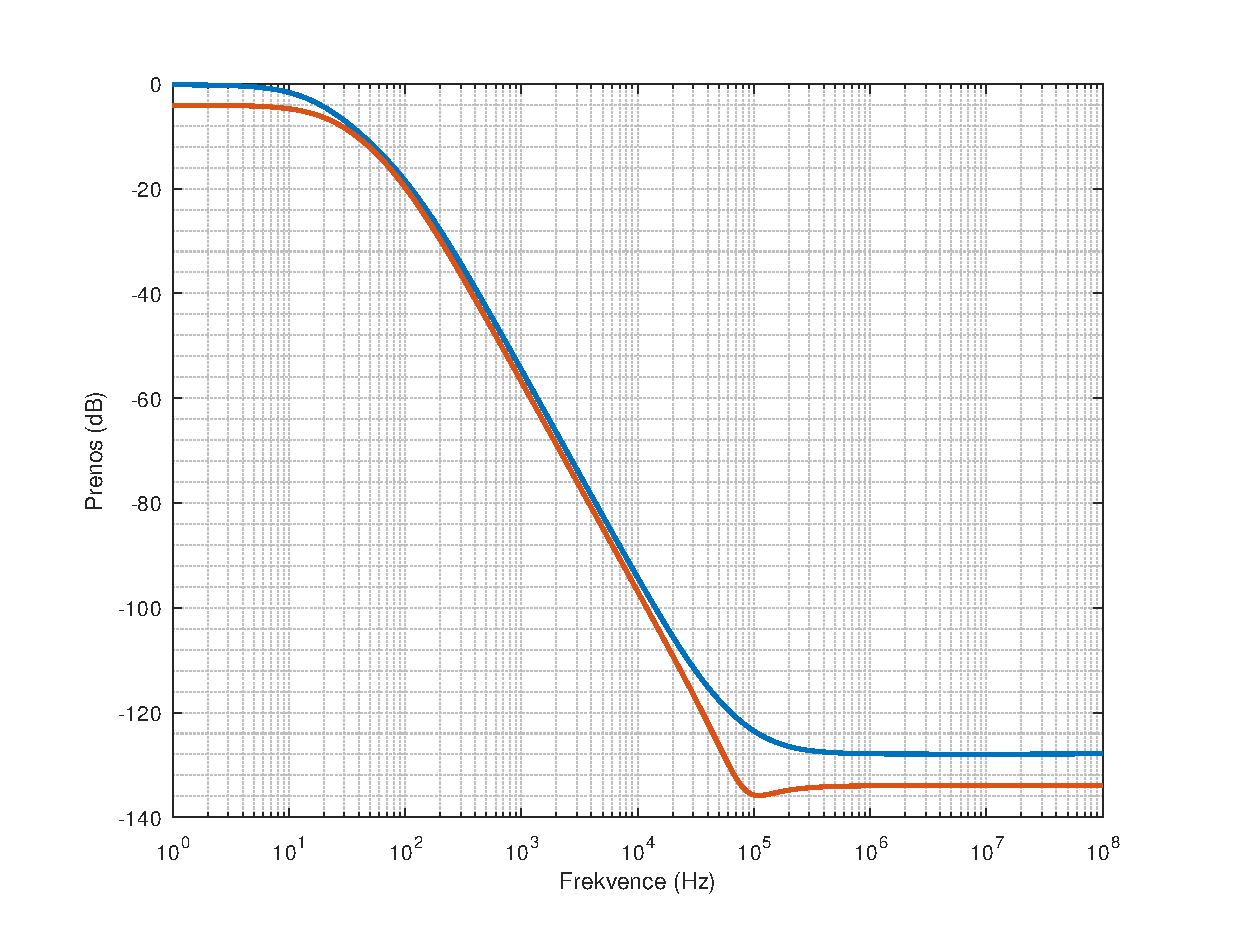
\includegraphics[width=\textwidth,keepaspectratio]{images/denoiser_transfer_function.eps}\caption{Přenosová charakteristika aktivních napájecích filtrů.}\label{analog_source_filter_transfer}
\end{figure}

\section{Digitalizace měřeného průběhu}
\chapter{Popis firmware}

Pojmem firmware je v této kapitole myšlen program, který běží v mikrokontroléru, obsluhuje všechny části reflektometru, poskytuje uživatelské rozhraní a zajišťuje měření, vyhodnocování měření a komunikaci s počítačem. Firmware je napsán v jazyce C, knihovny pro ovládání periferií byly převzaty od výrobce. Všechen ostatní zdrojový kód je vlastní, vznikl v rámci této práce.

\section{Technické parametry firmware}
Použitý mikrokontrolér disponuje \SI{20}{\kilo\byte} \acrshort{RAM}. Jeden měřený vzorek zabírá 12 bitů, bez použití komprese dat je možné do \acrshort{RAM} uložit 10000~vzorků. Parametr $\frac{a b}{c}$ v rovnici \ref{equation_tshift} určuje délku měřeného souboru dat. Vzhledem k použitým hodnotám má měřený soubor dat 500000~bodů s časovým krokem přibližně \SI{19.62}{\pico\second}. Část RAM ovšem zabírá program pro svůj chod, délka měřicího okna byla nakonec zvolena 4096 bodů, což umožňuje v rámci jednoho okna změřit interval o délce přes \SI{80}{\nano\second}. Ve vakuu tento interval odpovídá délce měřeného úseku \SI{12}{\meter}. Pro koaxiální kabely odpovídá měřený úsek přibližně \SIrange{7.9}{10.2}{\meter} při uvažování typického rozsahu zkracovacího činitele \SIrange{0.66}{0.85}{}. V případě potřeby měřit delší vedení se může měřicí okno posunout a měřit další úsek vedení. Tento nedostatek tedy nebrání měřit libovolně dlouhá vedení, pouze znamená, že pro delší vedení je nezbytné provádět měření po částech.

\section{Autokalibrace a autodiagnostika zařízení}

\subsection{Detekce stability fázového závěsu}
Po zapnutí mikrokontrolér zapne všechny svoje interní periferie, načež začne komunikovat s fázovým závěsem Si5351. Nejprve je kontrolován indikátor úspěšného startu fázového závěsu, firmware čeká, dokud není fázový závěs připraven. Firmware pak nakonfiguruje všechny registry fázového závěsu, ovšem prozatím je nastaven tak, aby negeneroval žádné řídicí signály. Následně kontroluje firmware diagnostické registry fázového závěsu pro zjištění, zda je stabilní krystalový oscilátor. Fázový závěs je schopen indikovat stav, kdy vysazuje krystalový oscilátor \cite{Si5351datasheet}, například kvůli nedostatečnému zisku oscilátoru. Dále jsou kontrolovány indikátory nestability fázového závěsu, která může být způsobena například špatně navrženým napájením obvodu, které má na pracovních frekvencích \acrshort{VCO} pak příliš vysokou impedanci (interní \acrshort{VCO} pracují ve frekvenčním rozsahu \SIrange{600}{900}{\mega\hertz}). Pokud během fáze testování nenastane žádná z popsaných chyb, pokračuje program dále, jinak se zastaví a informuje uživatele o chybě.

\subsection{Autokalibrace stejnosměrné složky}
Dalším krokem autokalibrace je nastavení stejnosměrného posuvu měřeného signálu. Tento krok je nezbytný kvůli rozptylu parametrů tranzistoru BF998 použitého v oddělovacím zesilovači, testuje se při odpojeném měřeném vedení. Fázovému závěsu se nyní zapnou všechny výstupy, není však generován budicí impulz, výstup obvodu je ovládán firmwarem. Nejprve je nastavena logická úroveň 1, firmware postupně inkrementuje kódové slovo \acrshort{DAC}, dokud se nedostane měřené napětí do měřitelného rozsahu. Pokud tento test selže, je opět indikována chyba. Výstup pro budicí impulz se přepne do logické úrovně 0. Ze změřených napětí se spočítá, jak je nezbytné dále posunout měřený signál tak, aby průměr napětí v obou stavech ležel uprostřed rozsahu ADC. Podle tohoto výsledku je kódové slovo DAC inkrementováno nebo dekrementováno, dokud není dosaženo požadovaného stavu.

\subsection{Kalibrace napěťových úrovní}
V dalším kroku se provede kalibrace logických úrovní a zjištění úrovně šumu v měřeném signálu. V obou logických úrovních budicího pulzu je nejprve změřeno 4096 vzorků, ze kterých se spočítá průměr. Potom se změří dalších 4096 vzorků, které jsou použity pro spočítání rozptylu měřených hodnot. Tím se získá informace o statických napěťových úrovních pro stavy odpovídající vedení zakončenému otevřeným koncem a zkratem, tedy pro koeficienty odrazu $-1$ a $+1$, čímž je získán teoretický rozsah měřených hodnot. Rozptyl hodnot je podstatný pro odhad vhodného počtu průměrování. Vhodný počet průměrování byl uvažován jako počet průměrů, při kterých již byl šum podstatně potlačen, avšak dále by jeho úroveň klesala již pomalu.

\subsection{Odhad šumové úrovně a průměrování}
Pro průměrování je použit algoritmus, který se v minulosti objevil např. v osciloskopech značky Hewlett-Packard \cite{HP54100_article_journal}. Tento algoritmus je počítán celočíselně a pro svůj chod potřebuje množství paměti odpovídající pouze jedinému zaznamenanému průběhu. Pro algoritmus je potřeba jen soubor předchozích změřených dat $ y_{i-1}$, nový změřený vzorek $x$ a proměnná $i$ vyjadřující, kolikátý průměr je právě měřen. Při změření nového $n$-tého vzorku se odpovídající $n$-tý zprůměrovaný vzorek získá podle rovnice \ref{equation_averaging}.

\begin{equation}
\begin{gathered}
	y_i[n]=	\frac{x[n]+i \cdot y_{i-1}[n]}{i+1}
\end{gathered}
\label{equation_averaging}
\end{equation}

Tento algoritmus byl numericky simulován, nejprve v přesné podobě v plovoucí desetinné čárce a poté v celočíselné podobě. Pro simulaci byla použita náhodná data s rozptylem 1024, a tedy směrodatnou odchylkou 32. Tato hodnota je blízká reálně měřeným hodnotám v realizovaném zapojení reflektometru. Graf \ref{averaging_variance} vychází z dat simulovaných v plovoucí desetinné čárce, pro celočíselnou variantu není graf uveden, neboť rozdíl mezi nimi není rozpoznatelný. Rozdíly jsou znázorněny na následujících grafech. Výpočty byly provedeny $256\times$, výsledky byly zprůměrovány, aby byly křivky v grafech hladké. Bez průměrování jsou křivky lehce zatížené šumem.

\begin{figure}[htbp]
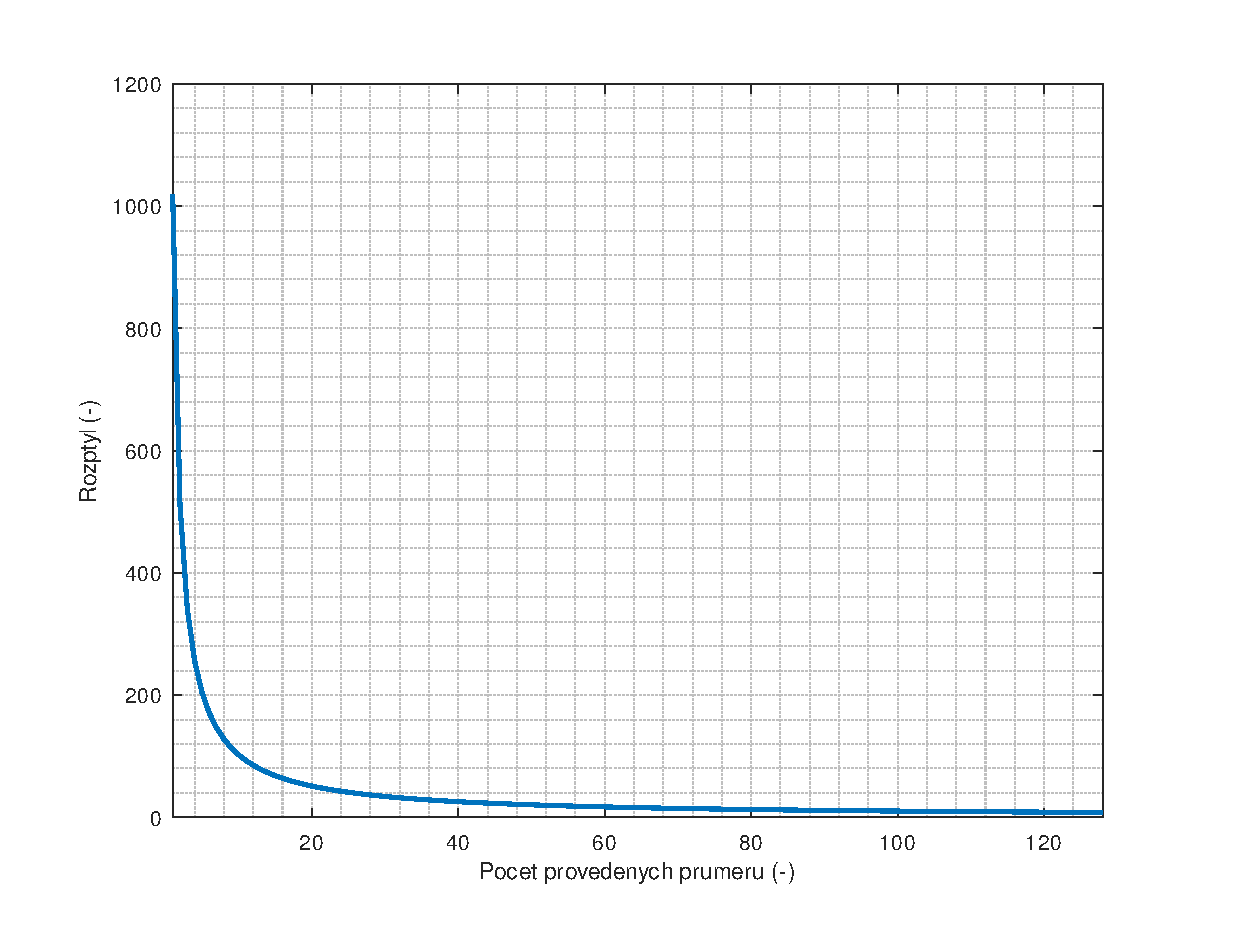
\includegraphics[width=\textwidth,keepaspectratio]{images/averaging_float_variance.eps}\caption{Závislost rozptylu na počtu provedených průměrů.}\label{averaging_variance}
\end{figure}	

Průběh této závislosti odpovídá funkci $\frac{1}{N}$, což je možné vizualizovat tak, že se rozptyl ve všech bodech pronásobí počtem průměrů, který danému bodu odpovídá. Na grafu \ref{averaging_float_difference_error} je vidět, že součin rozptylu s počtem průměrů je přibližně konstantní a odpovídá počátečnímu rozptylu. Diference rozptylu se pro větší počet průměrů než 16 blíží nule. Pro více než 16 průměrů, tedy polovinu směrodatné odchylky, tedy již úroveň šumu výrazně neklesá.

\begin{figure}[htbp]
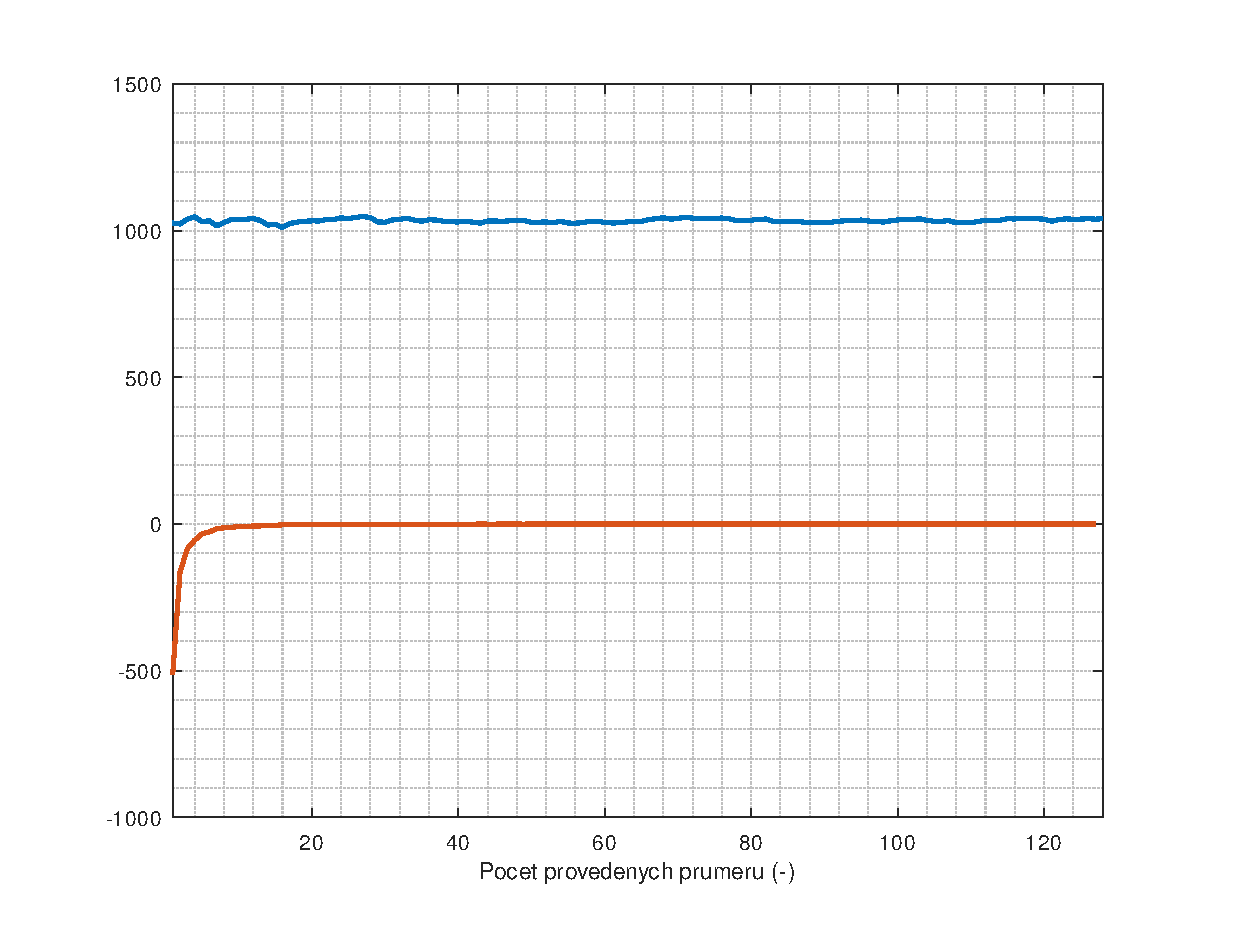
\includegraphics[width=\textwidth,keepaspectratio]{images/averaging_float_difference_error.eps}\caption{Závislost diference rozptylu (červeně) a součinu rozptylu s počtem průměrů (modře) na počtu provedených průměrů pro výpočet v plovoucí desetinné řádce.}\label{averaging_float_difference_error}
\end{figure}

\begin{figure}[htbp]
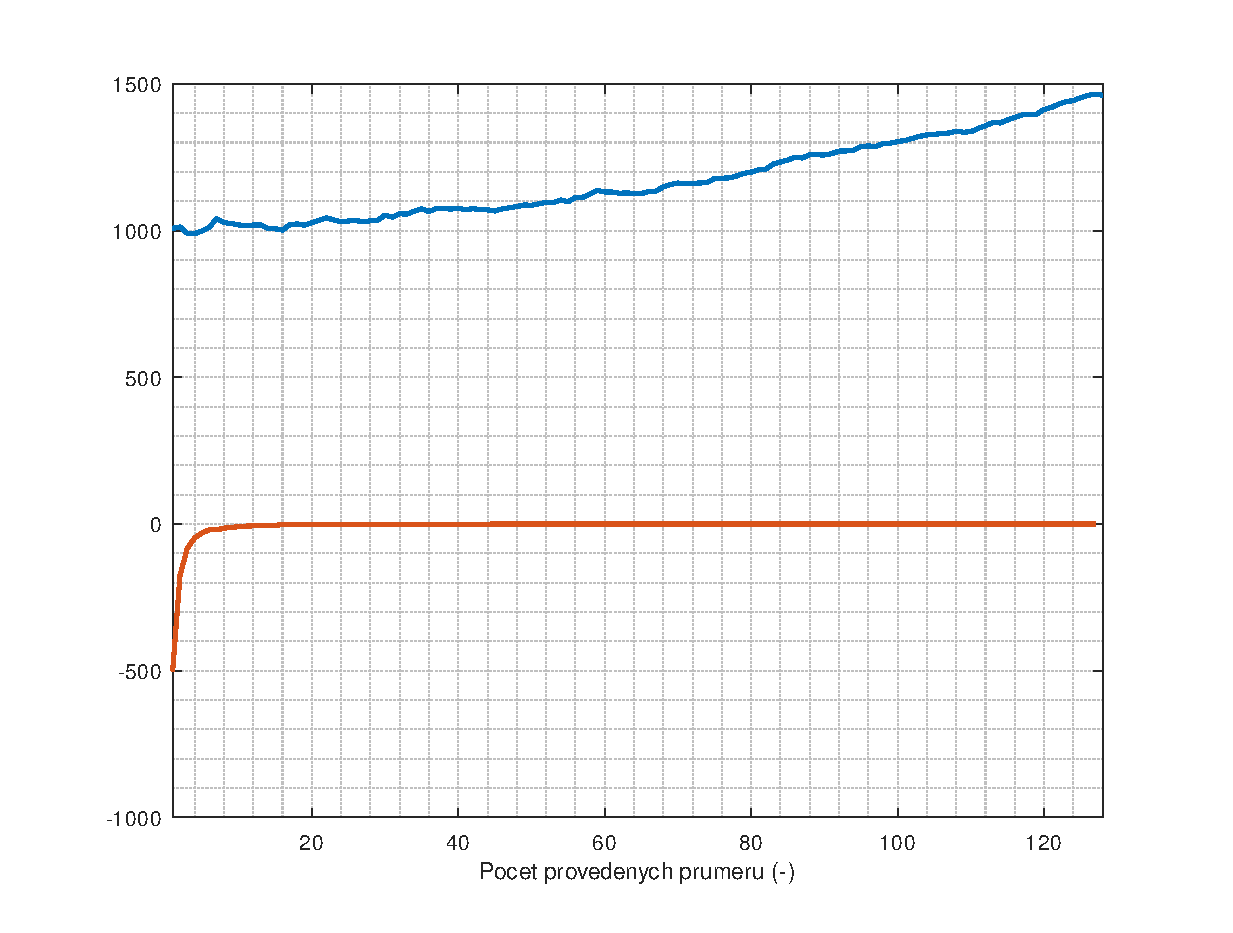
\includegraphics[width=\textwidth,keepaspectratio]{images/averaging_integer_difference_error.eps}\caption{Závislost diference rozptylu (červeně) a součinu rozptylu s počtem průměrů (modře) na počtu provedených průměrů pro celočíselné výpočty.}\label{averaging_integer_difference_error}
\end{figure}

V případě celočíselných výpočtů vypadá diference rozptylu podobně, ovšem ze součinu počtu průměrů a rozptylu je vidět, že závislost rozptylu na počtu průměrů neodpovídá již přesně hyperbolické funkci. Jde o vliv numerických chyb způsobovaných zaokrouhlováním výsledků. Pro větší počet průměrů než je směrodatná odchylka měřeného signálu, již znatelně stoupají numerické chyby. Význam tohoto faktu spočívá v tom, že již nestoupá odstup užitečného signálu od šumu, protože dominantním zdrojem šumu jsou chyby zaokrouhlování.

Výsledkem těchto simulací je odhad vhodného počtu průměru. Optimální počet průměrů $N$ tedy leží v rozsahu $\langle\frac{\sigma}{2}, \sigma \rangle$, kde $\sigma$ je směrodatná odchylka měřeného signálu. Po změření rozptylu měřeného signálu je tedy možné přímo odhadnout vhodný počet průměrování.

\subsection{Autokalibrace polohy budicího pulzu}
Při zapnutí fázového závěsu je fázový rozdíl mezi budicím signálem a vzorkovacím signálem náhodný. Proto je potřeba nejprve najít polohu budicího pulzu v měřených datech. Vzhledem k tomu, že není pro nedostatek RAM možné uložit celé měření a v uložených datech hledat budicí impulz, je využito přímého hledání náběžné hrany, kdy se ukládá pouze posledních 8 vzorků. Ta probíhá tak, že v obslužném přerušení se ukládá posledních 8 měřených vzorků, ze kterých se počítá průměr diferencí přes těchto 8 vzorků kvůli zvýšení imunity vůči šumu. Výpočet této průměrné diference je možné zjednodušit podle vzorce \ref{equation_difference_sum}. 

\begin{equation}
\begin{gathered}
	\mathit{diff}_{\mathrm{AVG8}}[n]= \dfrac{1}{8} \sum_{k=0}^7 \dfrac{x[n-k]-x[n-(k+1)]}{2}= \dfrac{x[n]-x[n-8]}{16}
\end{gathered}
\label{equation_difference_sum}
\end{equation}

Pak platí, že pro průměr $n$ diferencí je potřeba spočítat jen diferenci ze dvou vzorků vzdálených o~$n$~prvků. Tato operace tedy pro každý změřený vzorek vyžaduje jedinou matematickou operaci, a tedy zabere malé množství výpočetního času, díky čemuž je možné tento výpočet umístit do obslužného přerušení. Z tohoto spočteného průměru diferencí se hledá maximum, tedy oblast s nejvyšší strmostí. Během fáze hledání náběžné hrany je mimo přerušení sledována odhadnutá poloha náběžné hrany. Pokud se tato poloha čtyřikrát v řadě ocitne v tolerančním poli $\pm256$ bodů, je tato poloha uznána jako skutečná poloha náběžné hrany. Celá tato autokalibrační fáze probíhá s odpojeným měřeným systémem.

\begin{figure}[H]
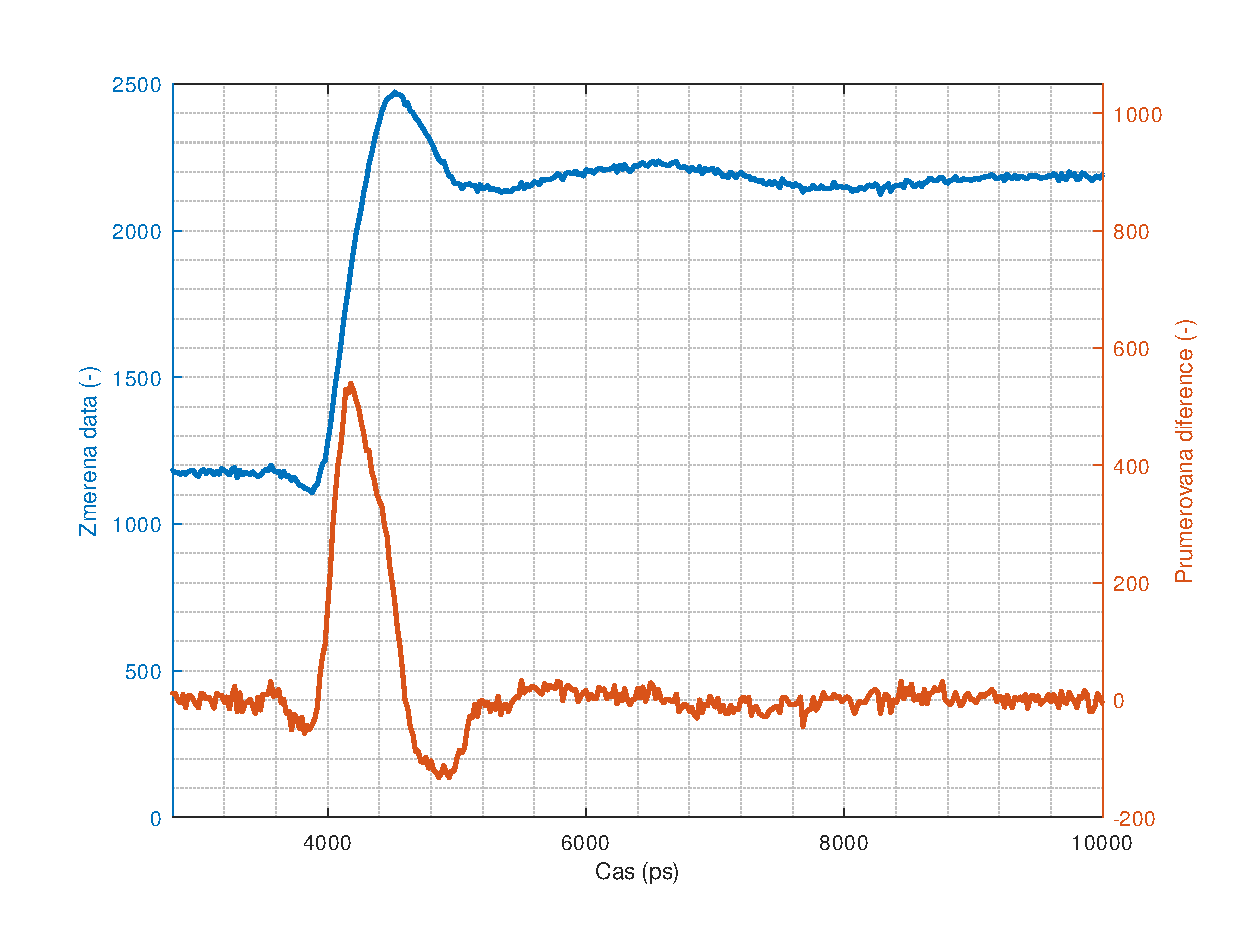
\includegraphics[width=\textwidth,keepaspectratio]{images/rising_edge_port_load.eps}\caption{Budicí pulz při připojeném standardu \quotedblbase load\textquotedblleft{} přímo k testovacímu portu. Červeně je vyznačena diference při průměrování přes 8 bodů. Maximum diference odpovídá přibližně středu náběžné hrany.}\label{rising_edge_port_load}
\end{figure}

\subsection{Kalibrace polohy roviny měření}
Následně je poloha měřicího okna nastavena 512 bodů před detekovanou hranu budicího pulzu. Reflektometr čeká na zásah uživatele, je vyžadováno připojení vedení, na jehož konec se později bude připojovat měřený systém. Na konec vedení je při tomto kalibračním kroku připojený kalibr typu \quotedblbase open\textquotedblleft. Průběh v okolí budicího pulzu je osmkrát změřen a zprůměrován. Ve změřeném průběhu je v oblasti odhadnuté náběžné hrany v rovině měření změřena počáteční napětí před náběžnou hranou a konečné napětí po náběžné hraně, odhad probíhá na základě maxima, ke kterému dochází na náběžné hraně v rámci překmitu. Následně proběhne hledání bodů, kde náběžná hrana prochází \SI{20}{\percent} a \SI{80}{\percent} mezi počátečním a konečným napětím. Z polohy těchto bodů je lineárně extrapolován počátek odezvy v rovině měření tak, aby při měření již nebyla měřena část sytému před rovinou měření. Budicí impulz je tedy po tomto kroku již mimo okno měření a nadále již v měření nijak nevystupuje. Ukázková odezva kalibru \quotedblbase open\textquotedblleft{} společně s vyznačenými význačnými body je na grafu \ref{rising_edge_DUT_open}.

\begin{figure}[H]
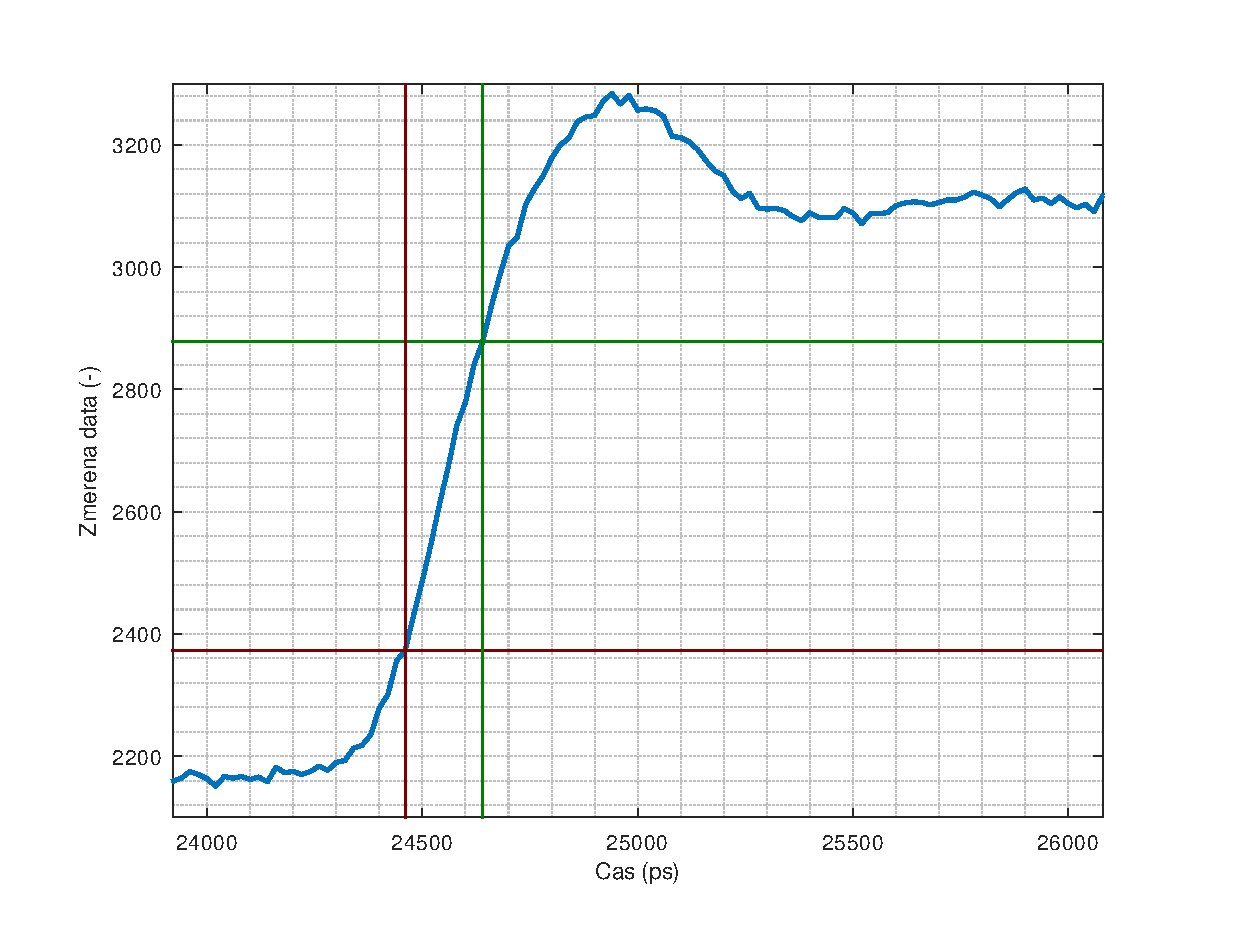
\includegraphics[width=\textwidth,keepaspectratio]{images/rising_edge_DUT_open.eps}\caption{Odezva v rovině měření při připojeném standardu \quotedblbase open\textquotedblleft , čáry vyznačují úrovně \SI{20}{\percent} (tmavě červená) a \SI{80}{\percent} (tmavě zelená) náběžné hrany a jejich polohu v čase. Délka náběžné hrany v tomto úseku je \SI{180}{\pico\second}. Při měření mezi body \SI{10}{\percent} a \SI{90}{\percent} náběžné hrany je tato délka \SI{280}{\pico\second}.}\label{rising_edge_DUT_open}
\end{figure}

\section{Postup ovládání firmware}
Po zapnutí se zobrazí obrazovka s informací o verzi firmware, datu a času jeho kompilace. Její podoba je vidět na obrázku \ref{greeting_screen}. Všechny dále uvedené obrázky byly vyexportovány z běžícího zařízení, měly by tedy přesně odpovídat zobrazovaným informacím.
\begin{figure}[H]
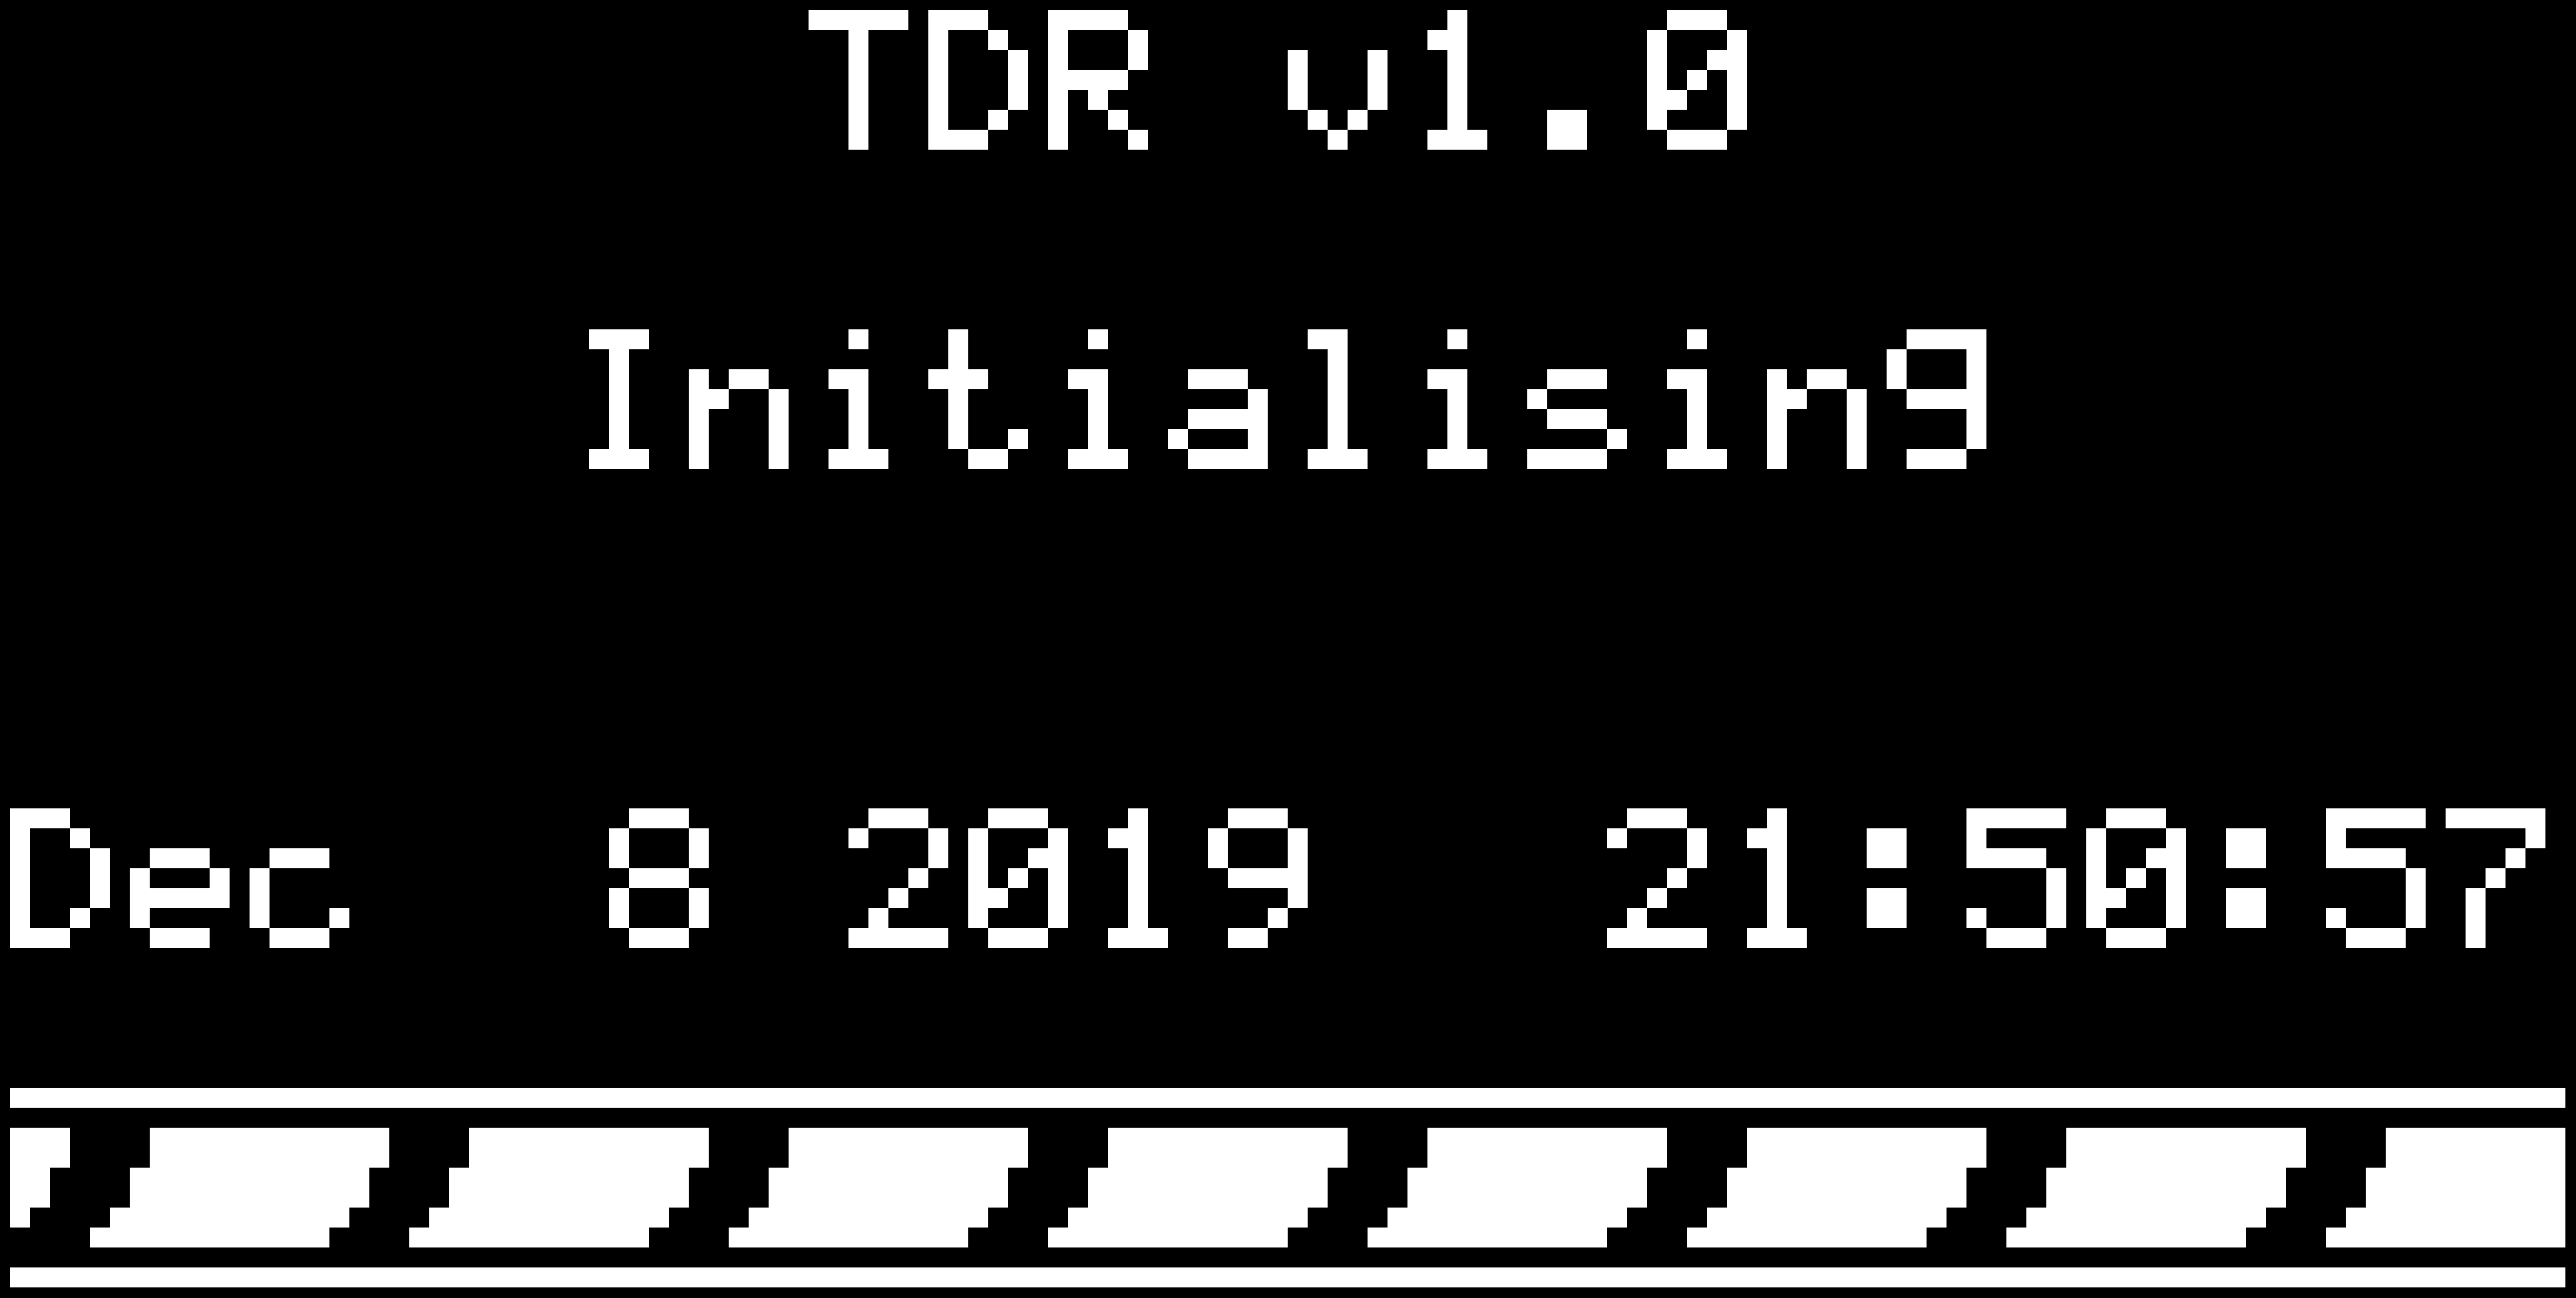
\includegraphics[width=0.3\textwidth,keepaspectratio]{images/greeting_screen.png}\caption{Uvítací obrazovka s informací o verzi.}\label{greeting_screen}
\end{figure}

Prozatím není zařízení interaktivní, pouze oznamuje stav autokalibračních postupů. Následuje detekce stability fázového závěsu, tuto část ukazují obrázky \ref{init_5351} a \ref{stability_5351}. Ukazatel ve spodní části je běžící, aby uživateli signalizoval, že zařízení běží a nezastavilo se například z důvodu nějaké chyby.
\begin{figure}[H]

\includegraphics[width=0.3\textwidth,keepaspectratio,interpolate=false]{images/init_5351.png}\caption{Obrazovka zobrazovaná po dobu inicializace fázového závěsu.}\label{init_5351}
\end{figure}

Po inicializaci následuje indikace stability jednotlivých částí PLL podle obrázku \ref{stability_5351}. V případě, že je vše v pořádku, zobrazí se hlášení \quotedblbase PLL Startup complete\textquotedblleft{} a program pokračuje dále. V případě, že dojde k chybě, program se zde zastaví s indikací chyby \quotedblbase PLL Startup error\textquotedblleft. 
\begin{figure}[H]
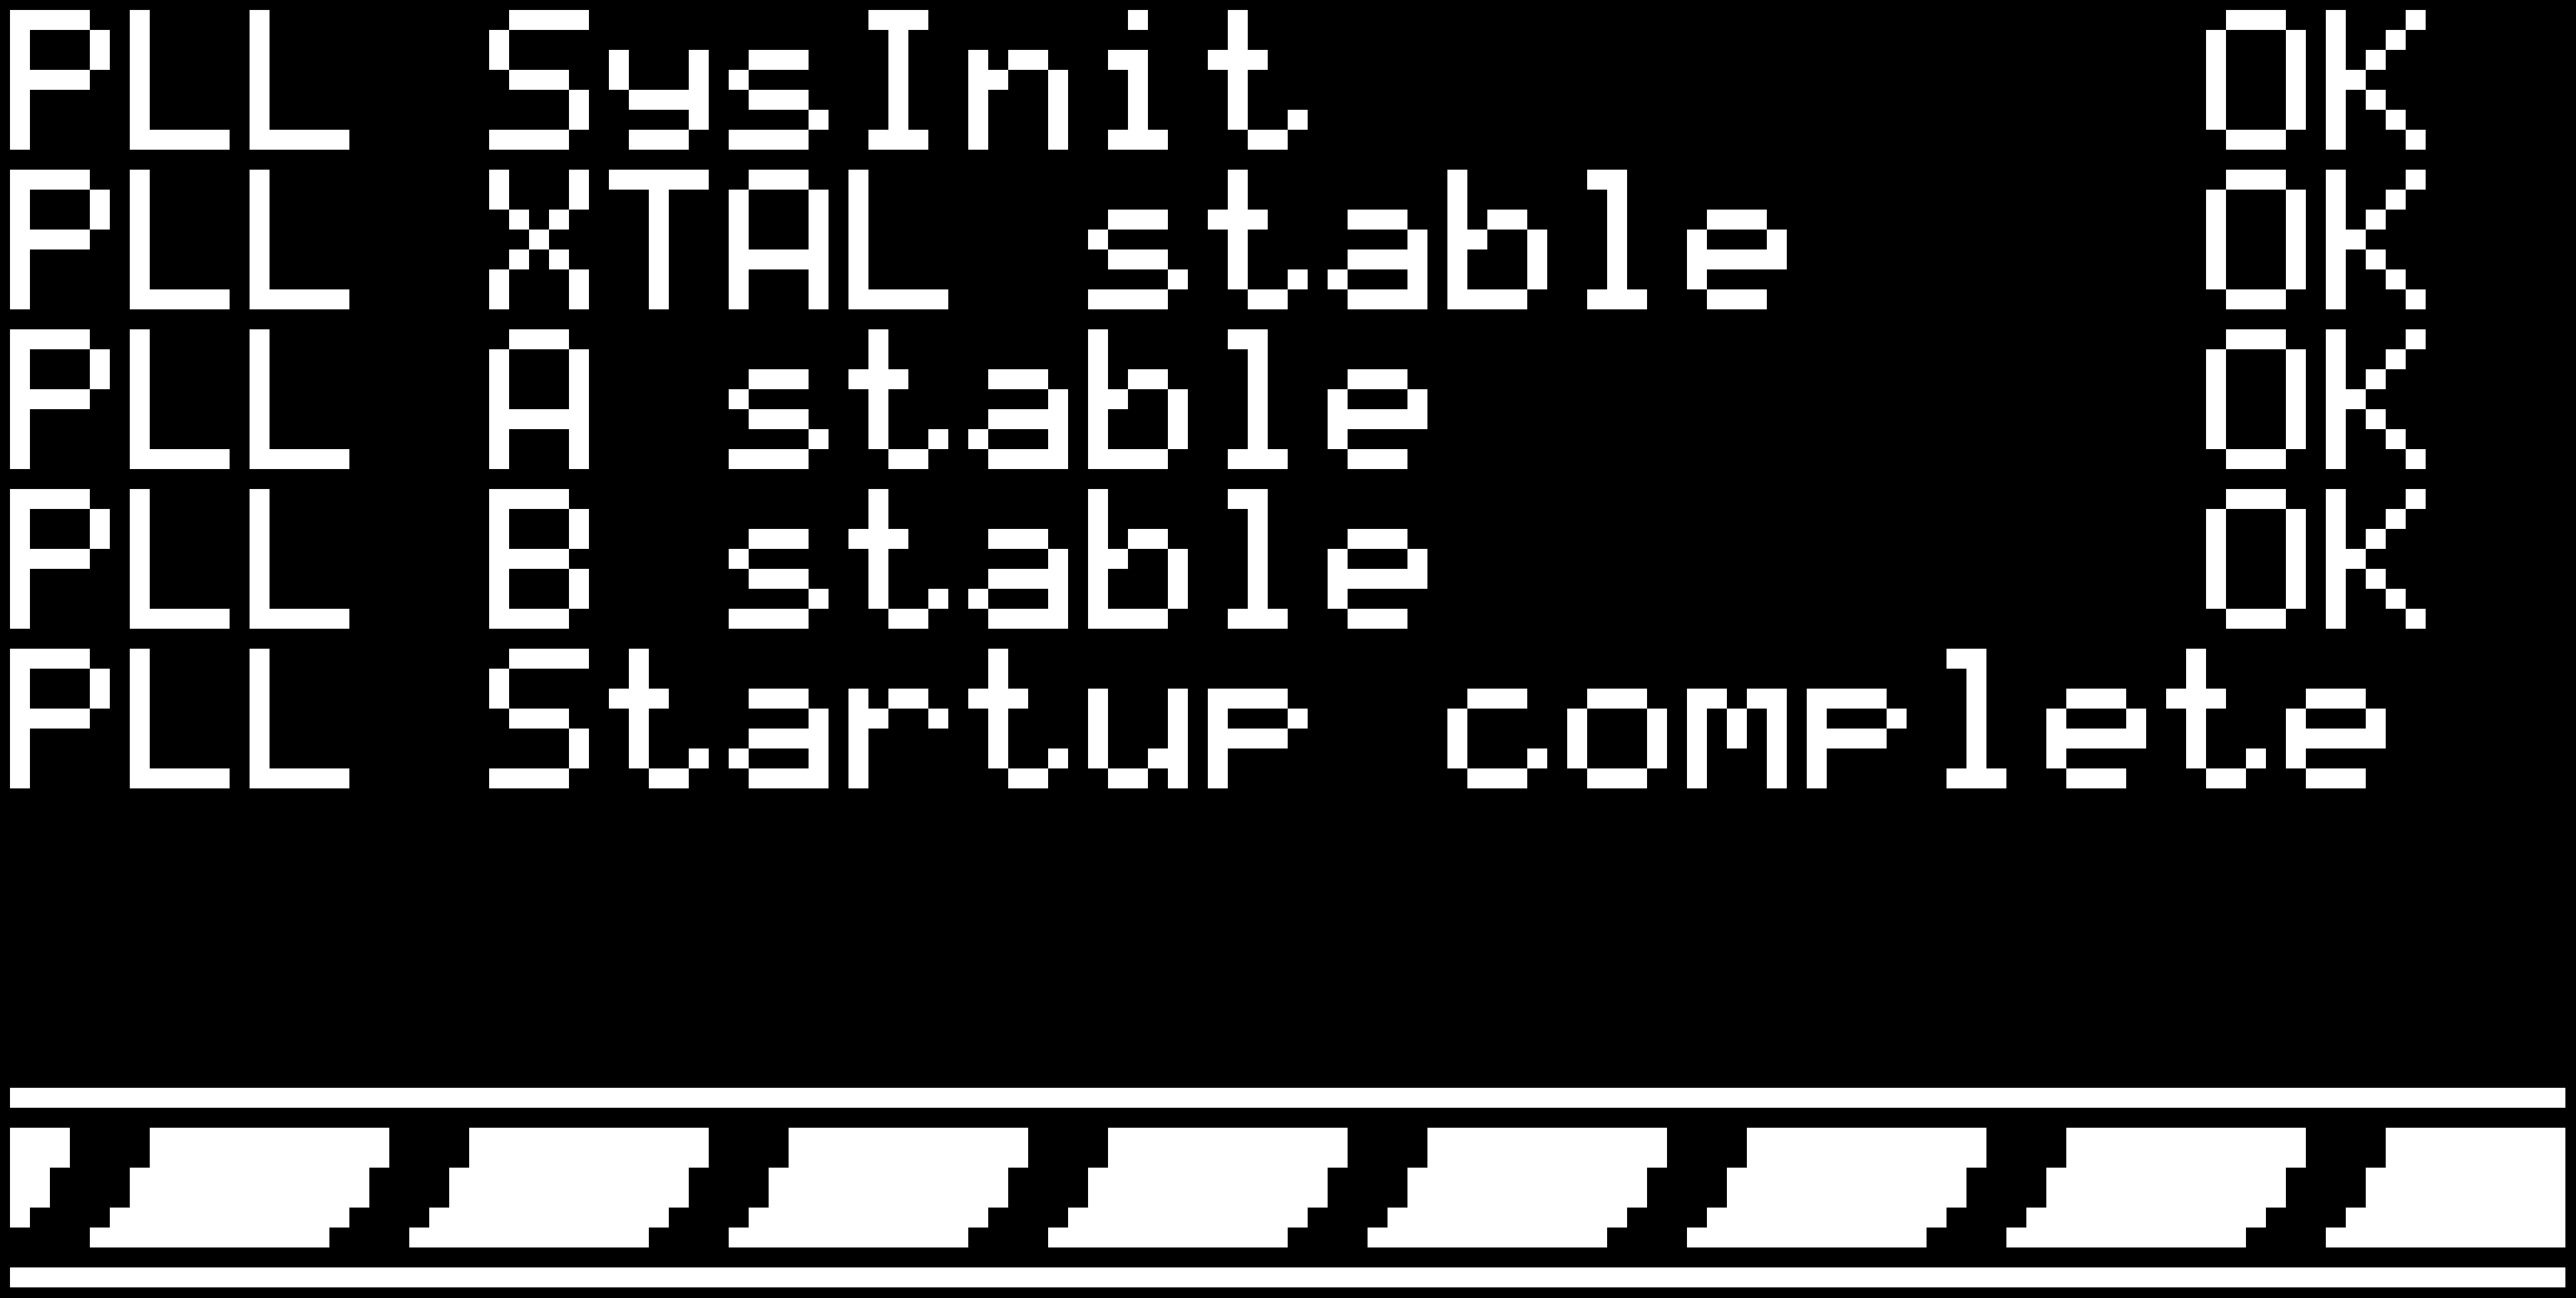
\includegraphics[width=0.3\textwidth,keepaspectratio,interpolate=false]{images/stability_5351.png}\caption{Obrazovka s informacemi o stabilitě jednotlivých částí PLL Si5351.}\label{stability_5351}
\end{figure}

Před autokalibrací polohy budicího pulzu, autokalibrací stejnosměrné složky a odhadu šumové úrovně je uživatel požádán, aby odpojil od reflektometru všechna připojená vedení nebo DUT. Tento požadavek je uveden na obr. \ref{offset_user_wait}. V tuto chvíli se zastaví běžící ukazatel ve spodní části obrazovky, aby signalizoval čekání.
\begin{figure}[H]
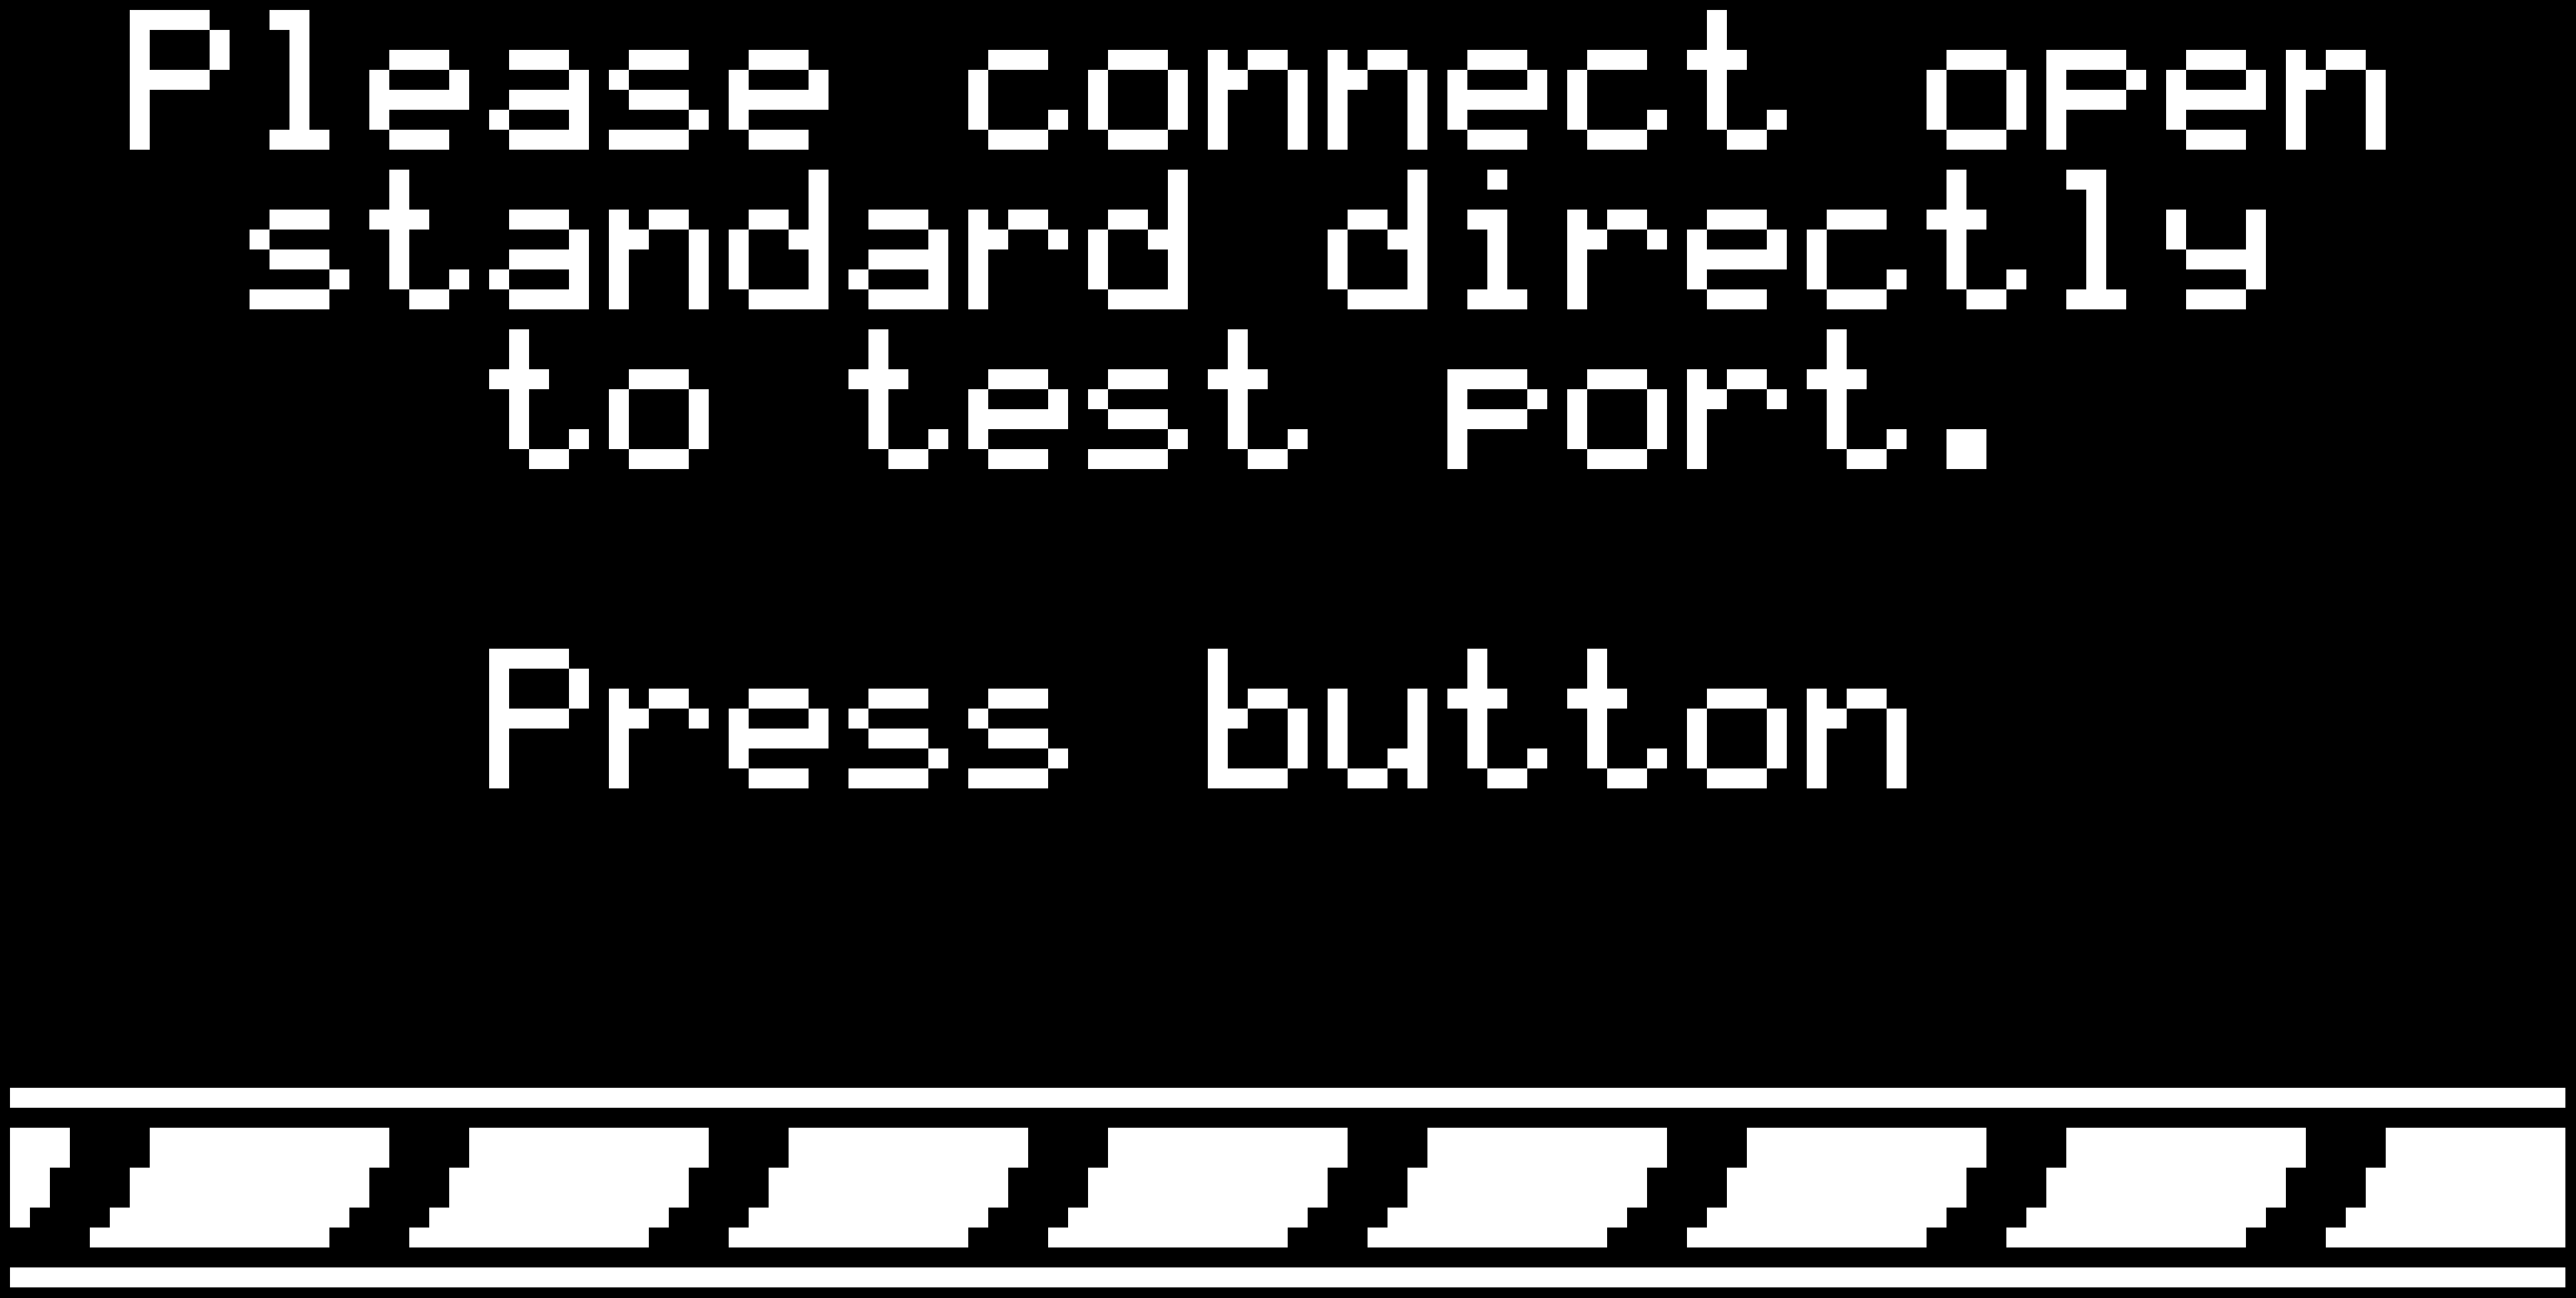
\includegraphics[width=0.3\textwidth,keepaspectratio,interpolate=false]{images/offset_user_wait.png}\caption{Čekání na zásah uživatele - autokalibrace stejnosměrné složky, kalibrace úrovní a měření úrovně šumu.}\label{offset_user_wait}
\end{figure}

V průběhu autokalibračních kroků je uživatel postupně informován o probíhajícím kroku, případně o jeho postupu. Takto proběhne autokalibrace stejnosměrné složky (obr. \ref{offset_wait}) a měření napěťových úrovní a úrovně šumu (obr. \ref{levels_user_wait}). Následně je uživatel informován o výsledku autokalibrace napěťových úrovní a šumu (obr. \ref{levels_complete}), ze kterých je možné odhalit některé možné závady. Pokud by například jedna z úrovní byla rovna 0 nebo 4095, případně kdyby se obě přibližně rovnaly, pak je možné usuzovat na chybu ADC nebo hardwarovou závadu. Pokud by vyšla variance měřeného signálu příliš vysoká nebo příliš nízká, mohla by tato informace indikovat chybu vzorkovače.
\begin{figure}[H]
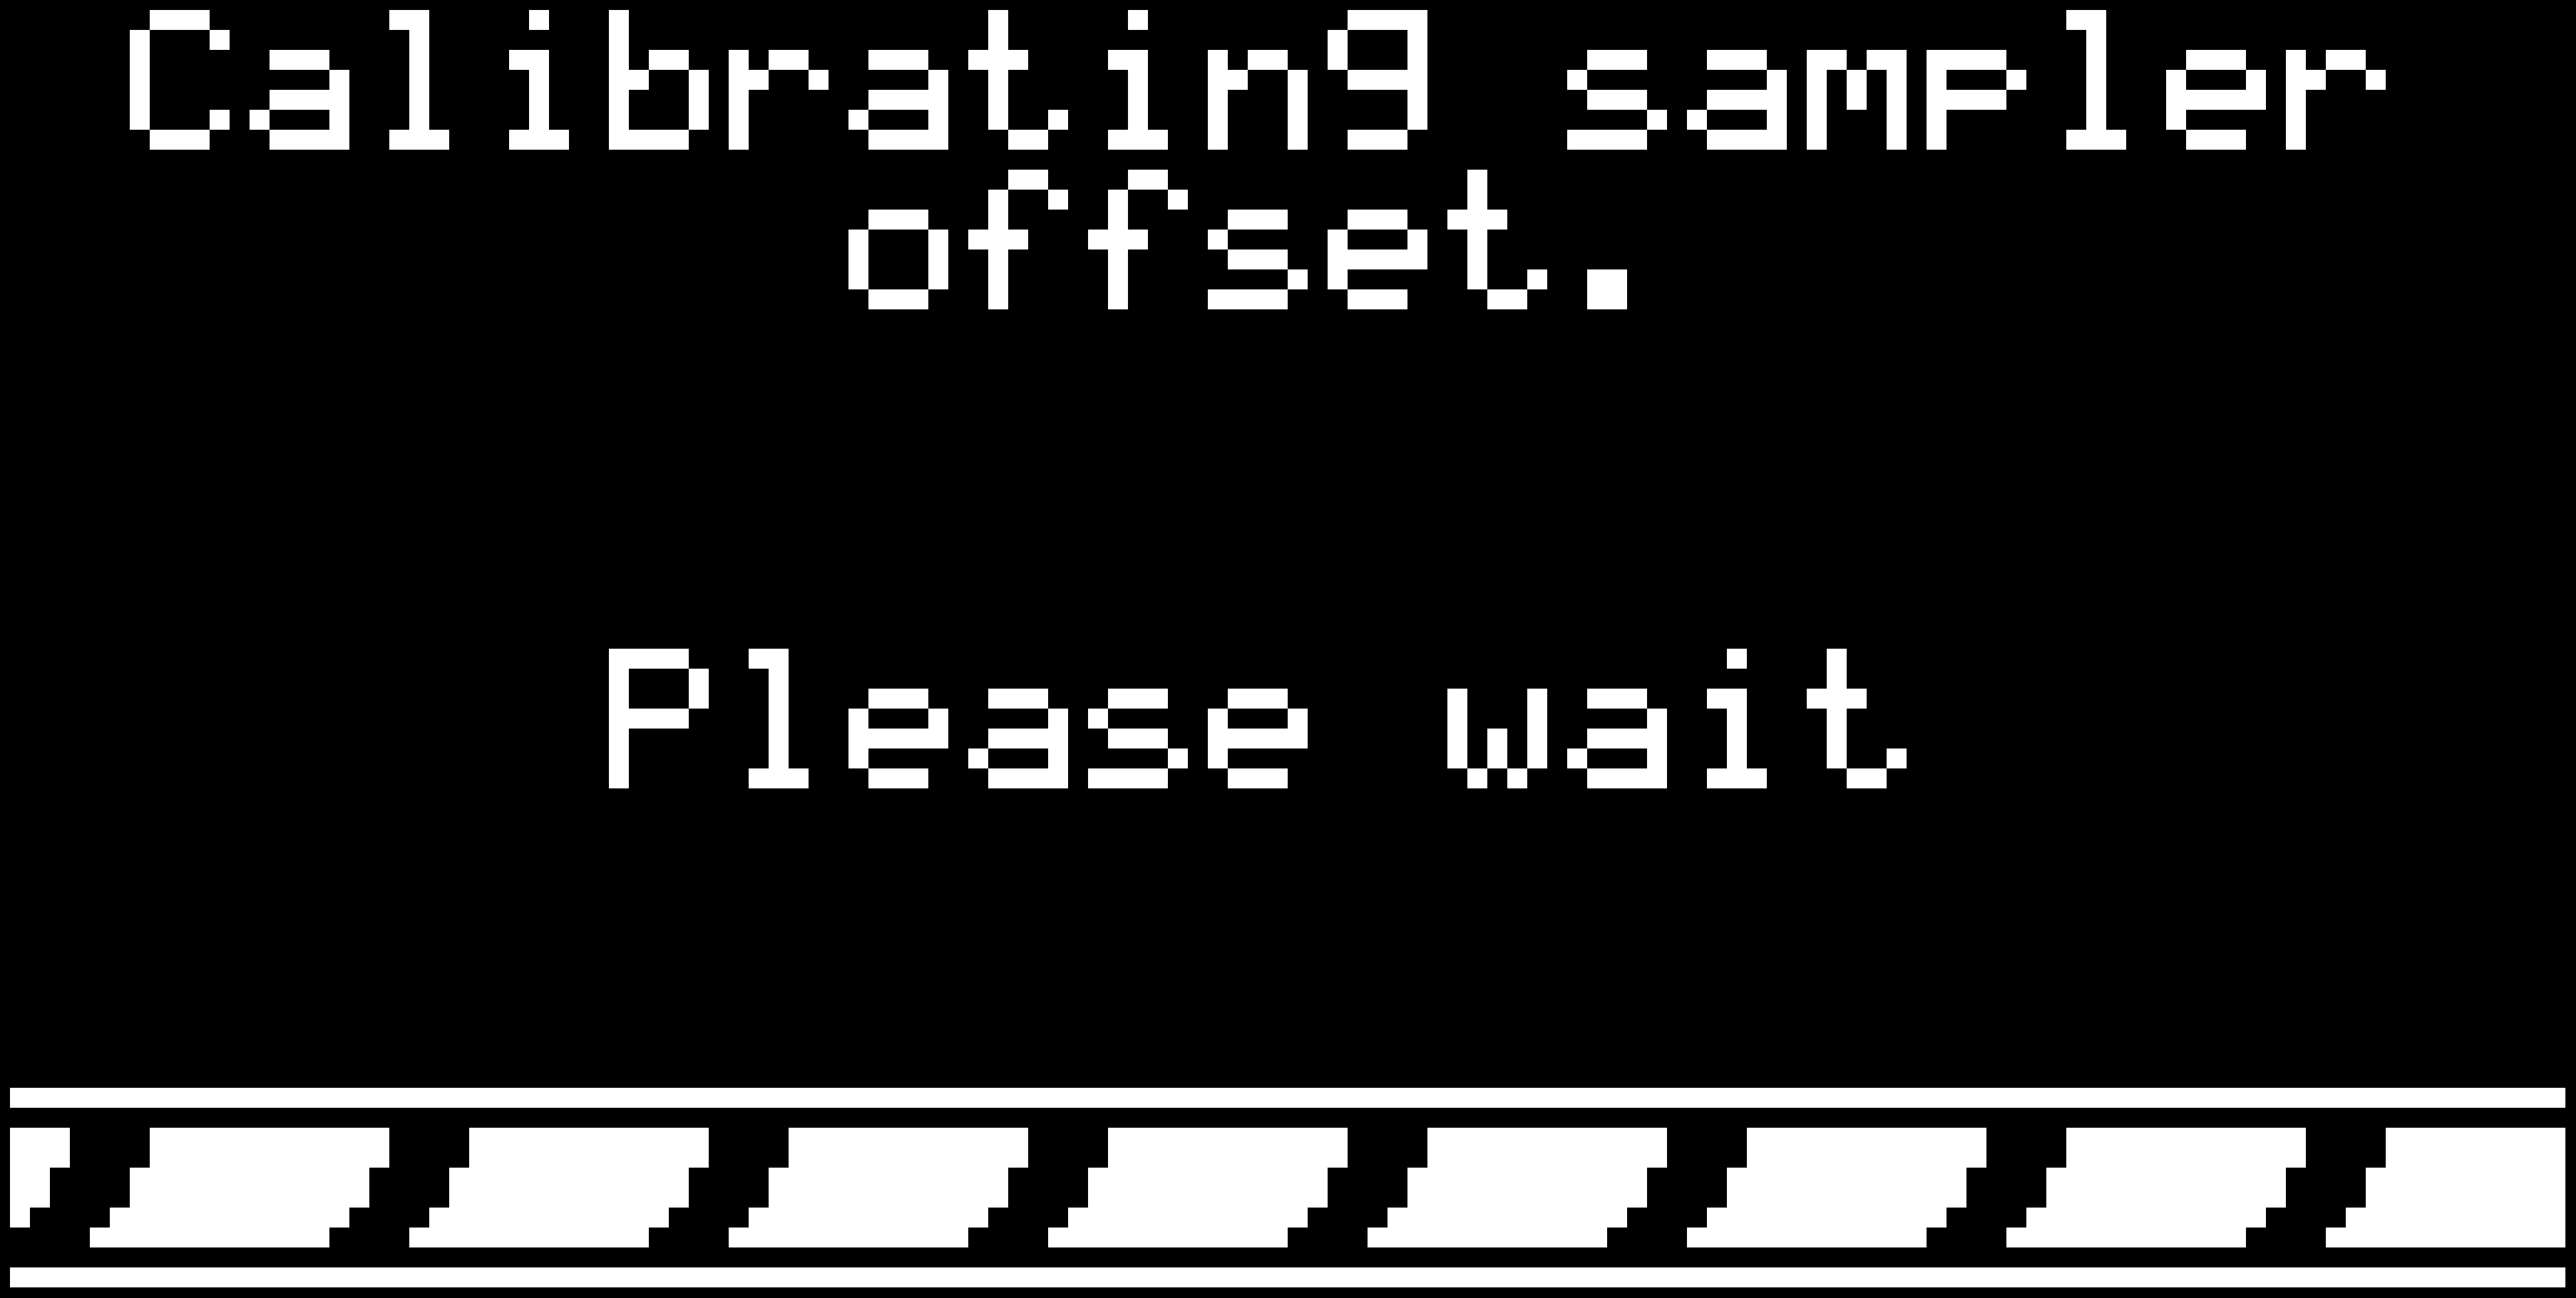
\includegraphics[width=0.3\textwidth,keepaspectratio,interpolate=false]{images/offset_wait.png}\caption{Probíhající autokalibrace stejnosměrné složky.}\label{offset_wait}
\end{figure}

\begin{figure}[H]
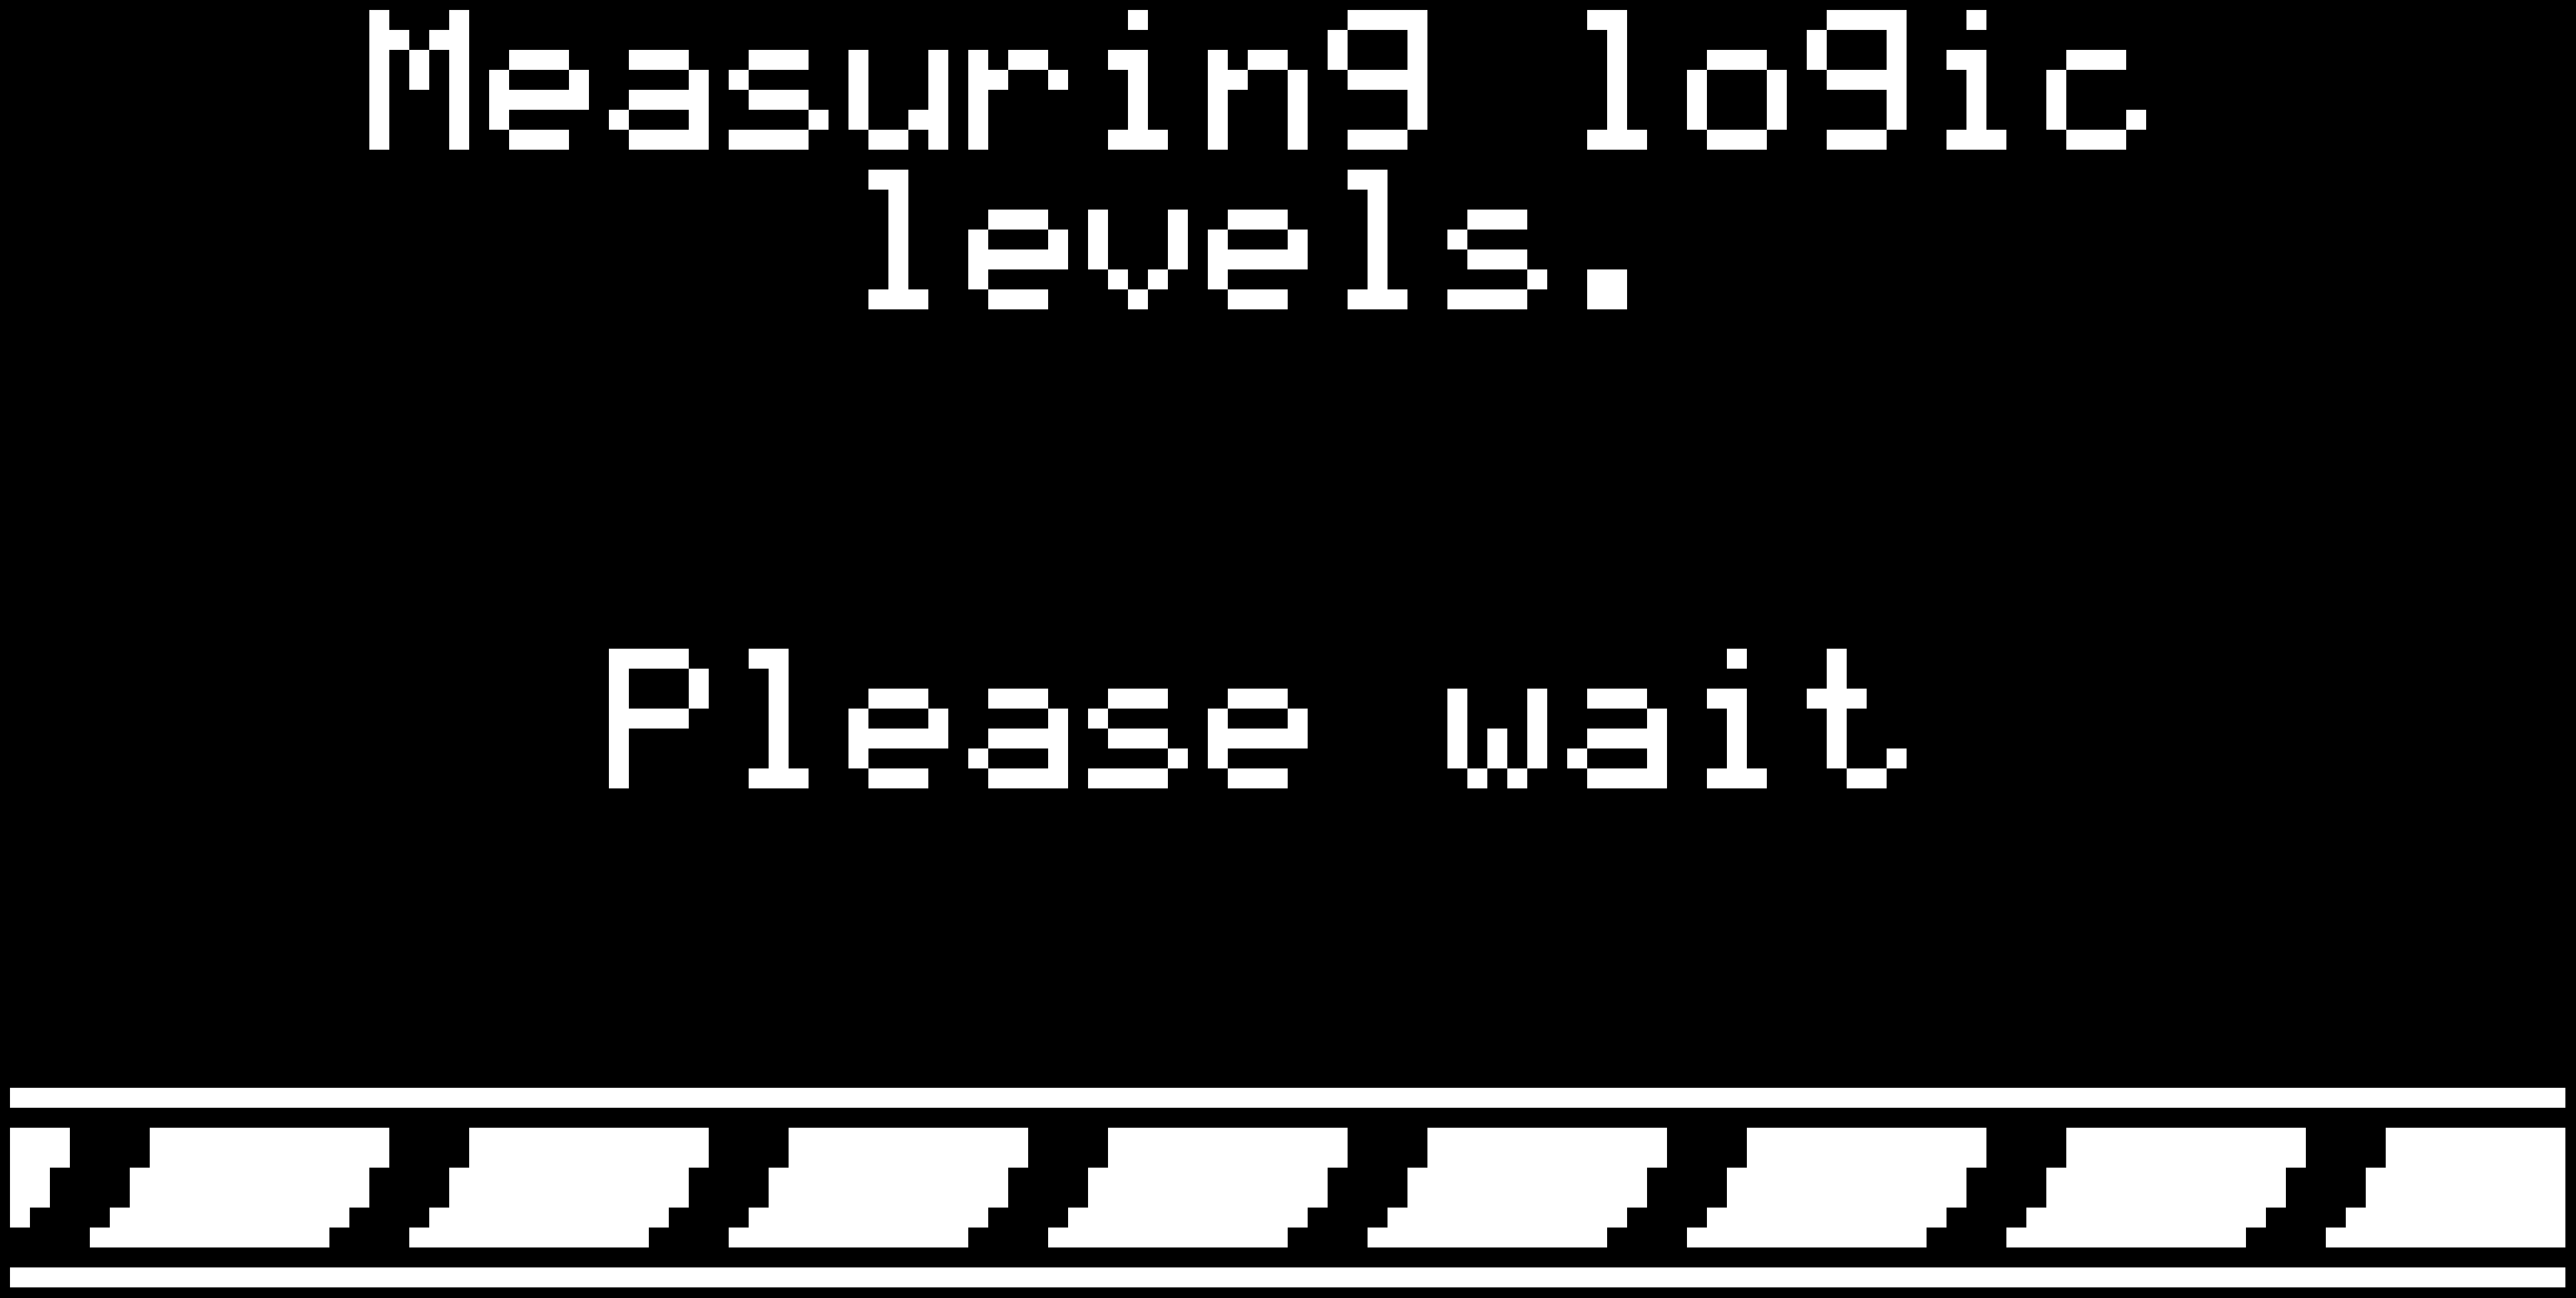
\includegraphics[width=0.3\textwidth,keepaspectratio,interpolate=false]{images/levels_user_wait.png}\caption{Probíhající autokalibrace napěťových úrovní a měření úrovně šumu.}\label{levels_user_wait}
\end{figure}

\begin{figure}[H]
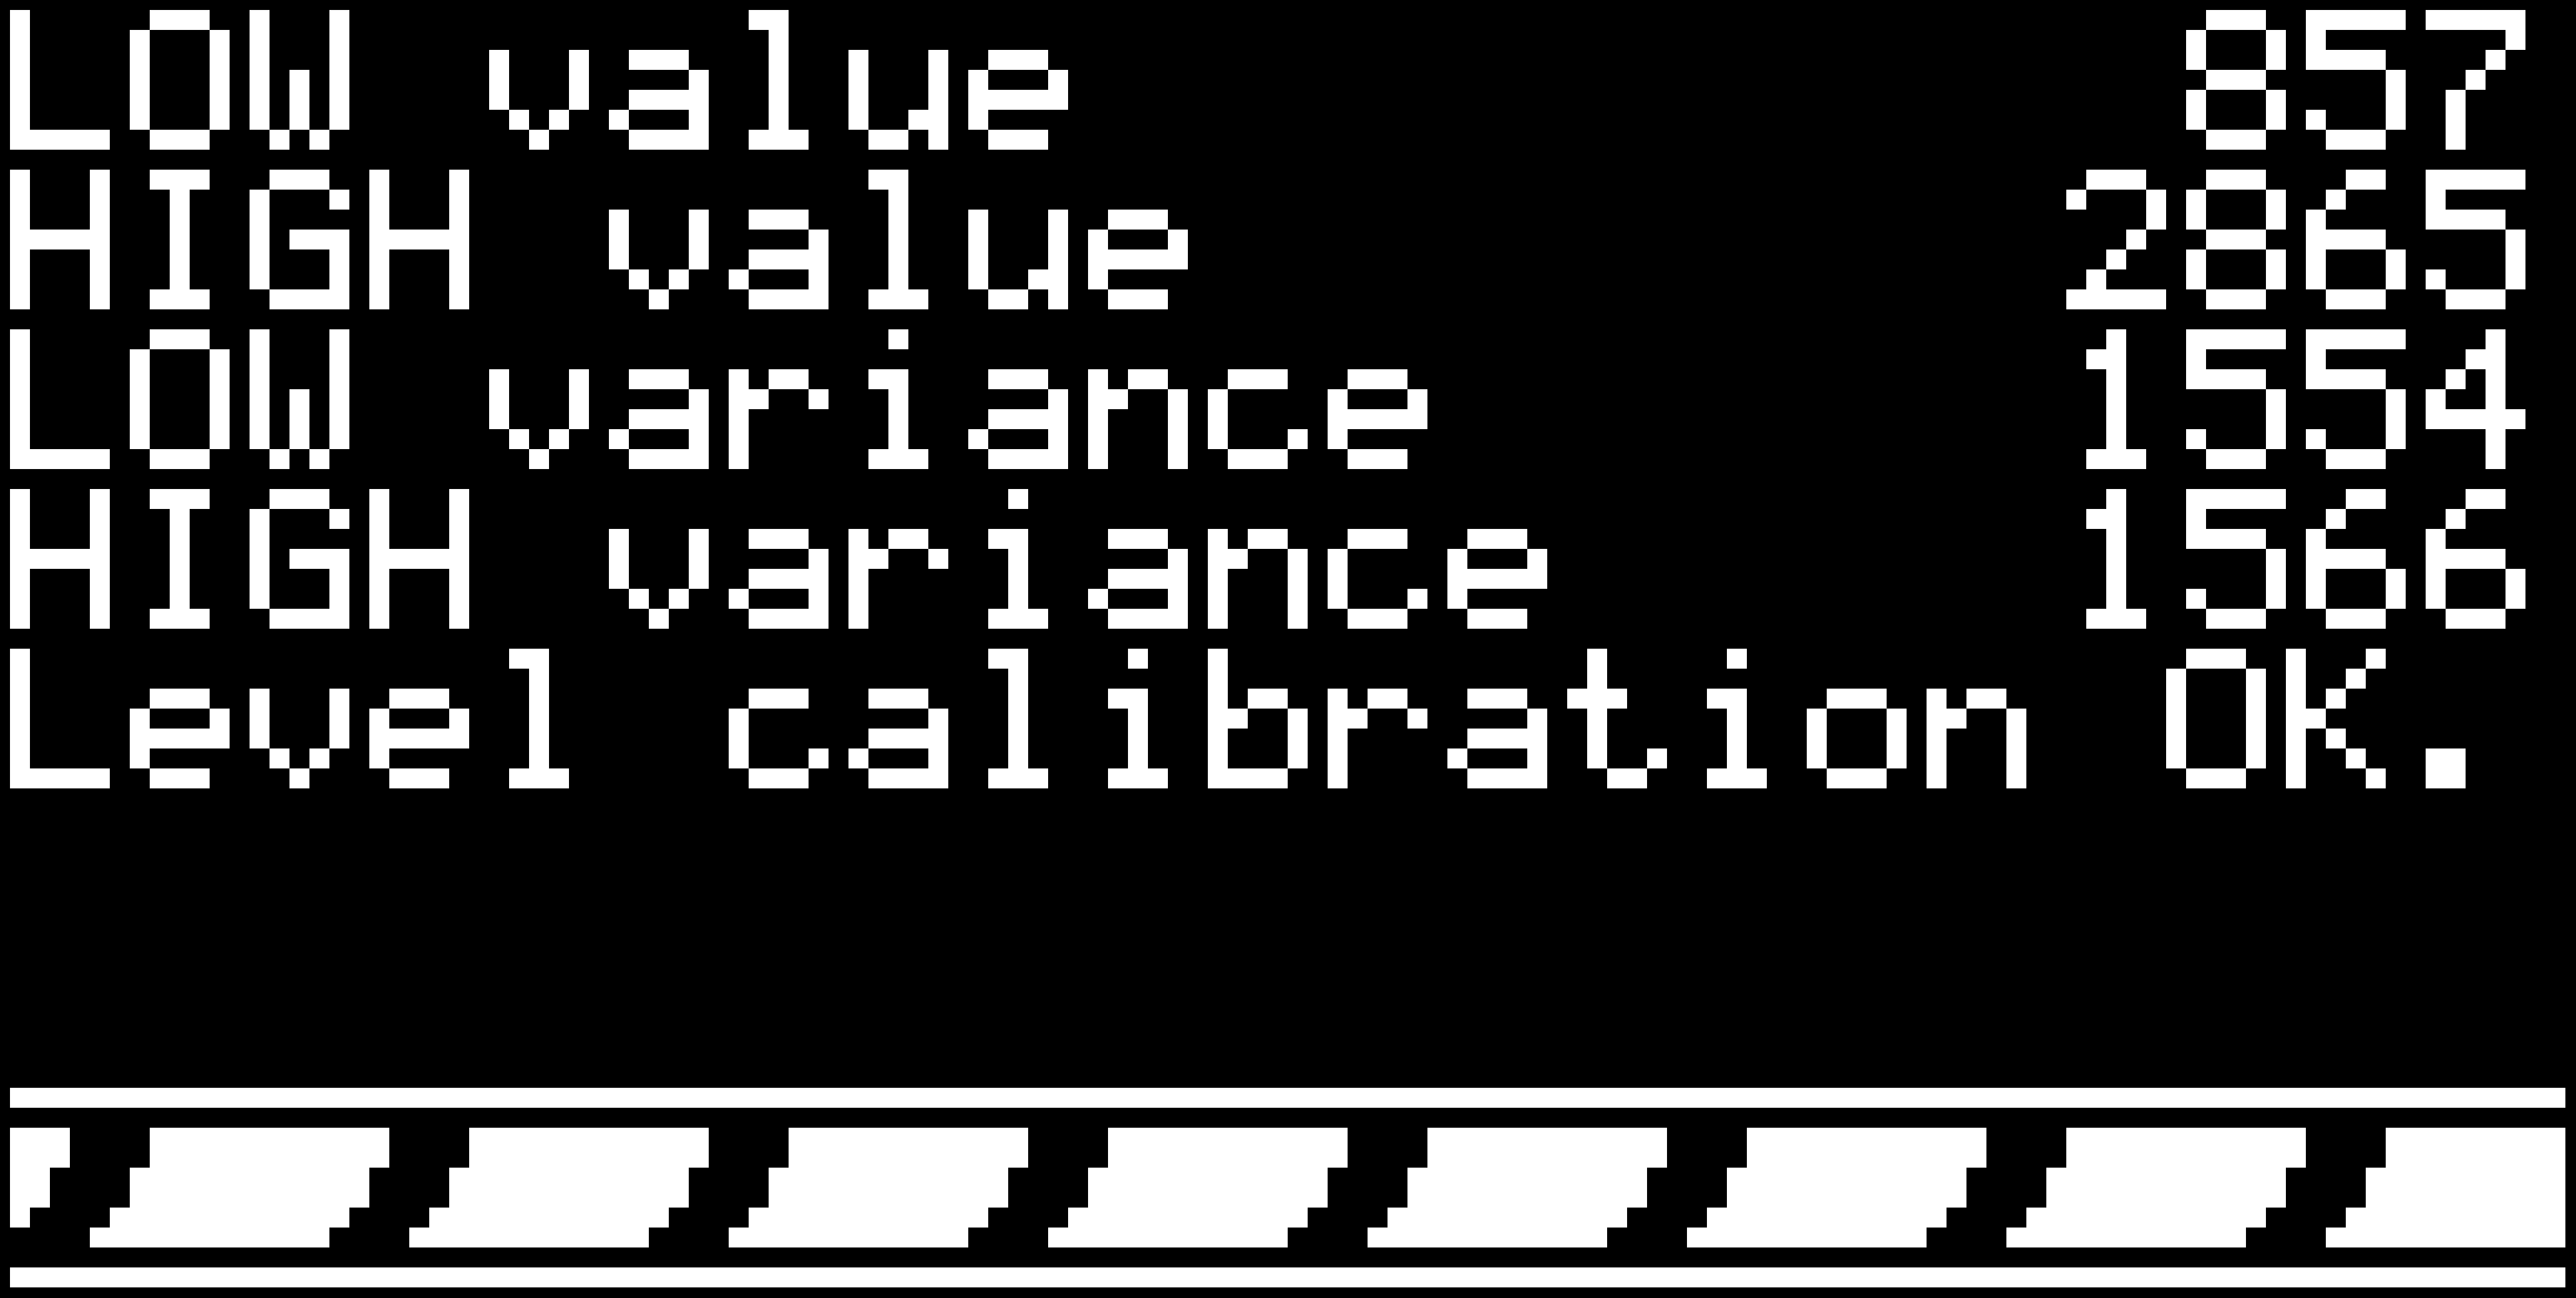
\includegraphics[width=0.3\textwidth,keepaspectratio,interpolate=false]{images/levels_complete.png}\caption{Výsledek autokalibrace napěťových úrovní a měření šumu.}\label{levels_complete}
\end{figure}

Po změření napěťových a šumových úrovní následuje hrubé hledání náběžné hrany budicího signálu, indikováno je dle obr. \ref{edge_wait}.
\begin{figure}[H]
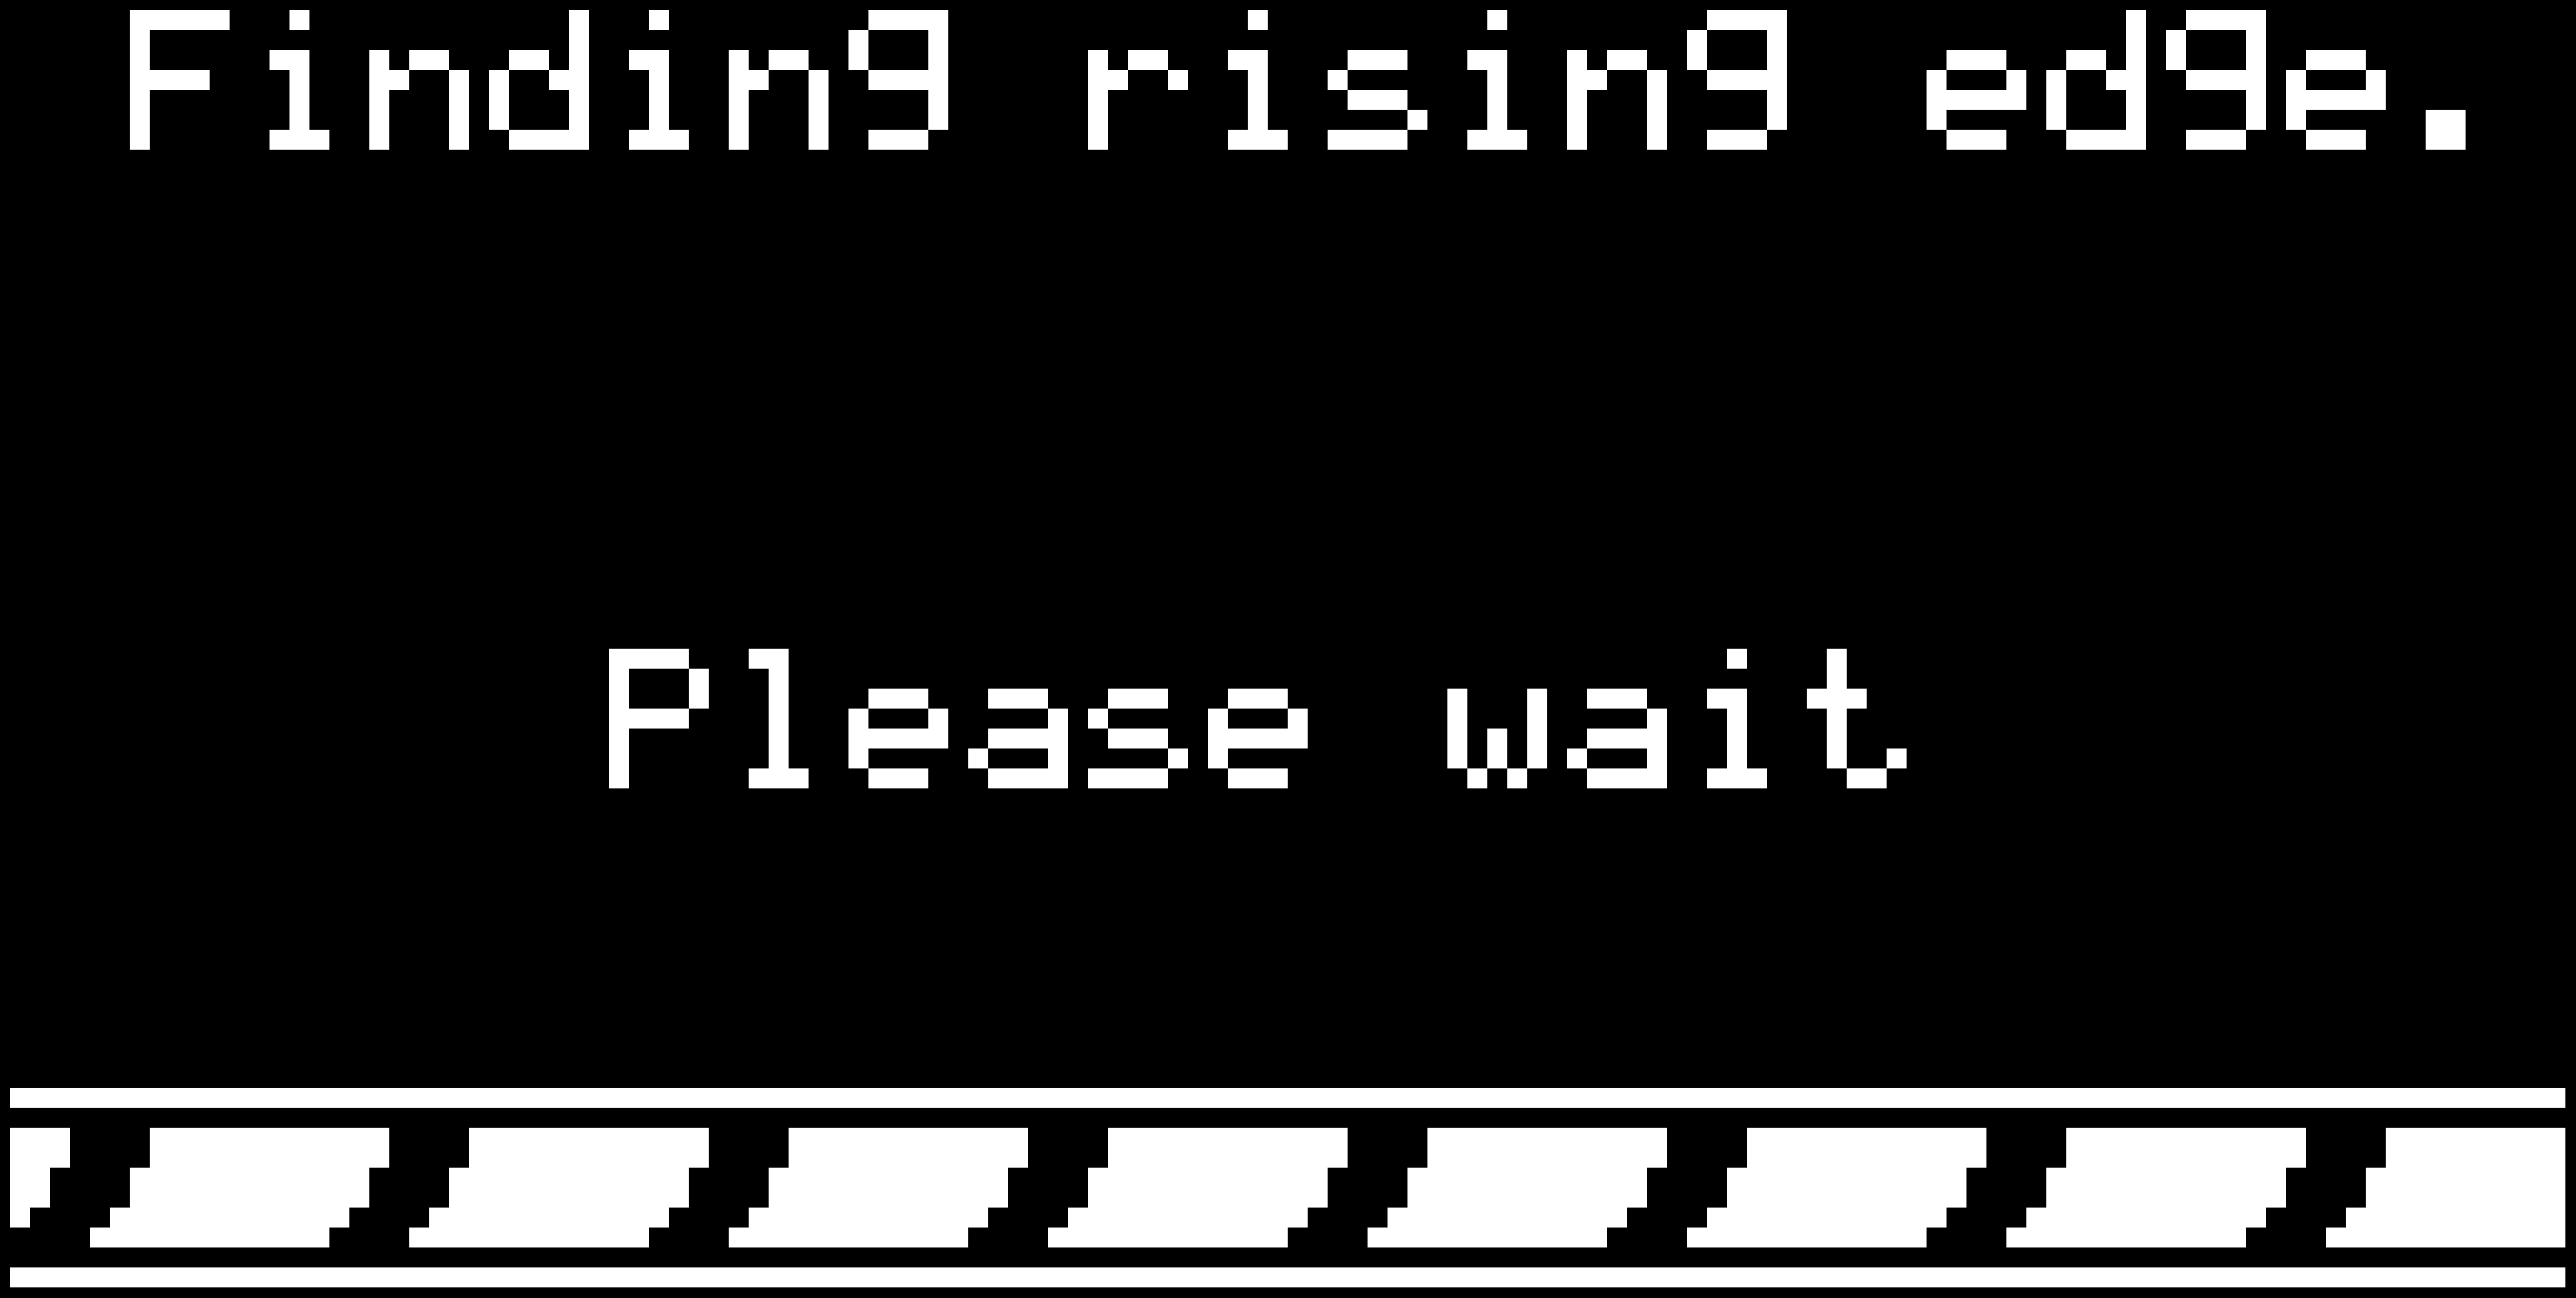
\includegraphics[width=0.3\textwidth,keepaspectratio,interpolate=false]{images/edge_wait.png}\caption{Hrubé hledání náběžné hrany.}\label{edge_wait}
\end{figure}

Po hrubém nalezení polohy hrany budicího signálu je uživatel vyzván k připojení testovacího vedení a připojení standardu \quotedblbase open\textquotedblleft{} na konec vedení podle obr. \ref{edge_user_wait}.
\begin{figure}[H]
\includegraphics[width=0.3\textwidth,keepaspectratio,interpolate=false]{images/edge_user_wait.png}\caption{Čekání na zásah uživatele - přesné hledání náběžné hrany.}\label{edge_user_wait}
\end{figure}

Přesné hledání polohy měřicí roviny trvá delší dobu, protože dochází k opakovanému měření a průměrování. Tento proces je tedy indikován ukazatelem průběhu, ze kterého je možné odhadnout, kdy bude proces dokončen. Tento krok je uveden na obr. \ref{edge_sampling}. Po dokončení hledání je zobrazeno potvrzení o úspěšném dokončení autokalibrace podle obr. \ref{edge_found}.
\begin{figure}[H]
\includegraphics[width=0.3\textwidth,keepaspectratio,interpolate=false]{images/edge_sampling.png}\caption{Přesné hledání náběžné hrany.}\label{edge_sampling}
\end{figure}

\begin{figure}[H]
\includegraphics[width=0.3\textwidth,keepaspectratio,interpolate=false]{images/edge_found.png}\caption{Úspěšné nalezení přesné polohy náběžné hrany.}\label{edge_found}
\end{figure}

Nyní je již zařízení připraveno k měření. Uživatel je dle obr. \ref{measurement_user_wait} vyzván k připojení DUT a potvrzení začátku měření tlačítkem.
\begin{figure}[H]
\includegraphics[width=0.3\textwidth,keepaspectratio,interpolate=false]{images/measurement_user_wait.png}\caption{Čekání na zásah uživatele - připojení DUT a začátek měření.}\label{measurement_user_wait}
\end{figure}

Během prvního měření je zobrazena informace o čekání na dokončení prvního měření dle obr. \ref{measurement_avg_wait}.
\begin{figure}[H]
\includegraphics[width=0.3\textwidth,keepaspectratio,interpolate=false]{images/measurement_avg_wait.png}\caption{Čekání na proběhnutí prvního měření.}\label{measurement_avg_wait}
\end{figure}

V průběhu dalších měření je průběh každého měření indikován ukazatelem v levé spodní části obrazovky dle obr. \ref{measurement_running} a celkový počet změřených průběhů je uveden v pravé spodní části obrazovky. Změřený a zprůměrovaný průběh je vidět v horní části obrazovky.
\begin{figure}[H]
\includegraphics[width=0.3\textwidth,keepaspectratio,interpolate=false]{images/measurement_running.png}\caption{Průběh měření, 33. průměr.}\label{measurement_running}
\end{figure}

V případě, že je zařízení ovládáno z počítače, je na konci měření zobrazena výzva k vyčkání na odeslání zprůměrovaných změřených dat do počítače. Tato výzva je vyobrazena na obr. \ref{measurement_complete}.
\begin{figure}[H]
\includegraphics[width=0.3\textwidth,keepaspectratio,interpolate=false]{images/measurement_complete.png}\caption{Měření dokončeno.}\label{measurement_complete}
\end{figure}

V případě, že je zařízení ovládáno bez využití počítače, přiblíží se změřená data tak, aby každý změřený bod odpovídal jednomu horizontánímu bodu na displeji. Začátek tohoto procesu je zachycen na obr. \ref{zooming_start}, konec tohoto procesu pak na obr. \ref{zooming_complete}.
\begin{figure}[H]
\includegraphics[width=0.3\textwidth,keepaspectratio,interpolate=false]{images/zooming_start.png}\caption{Měření dokončeno, začátek přibližování změřených dat.}\label{zooming_start}
\end{figure}

\begin{figure}[H]
\includegraphics[width=0.3\textwidth,keepaspectratio,interpolate=false]{images/zooming_complete.png}\caption{Měření dokončeno, konec přibližování změřených dat.}\label{zooming_complete}
\end{figure}

Po přiblížení se změřený průběh začne plynule posouvat až k části průběhu, kde byla detekována diskontinuita na vedení podle obr. \ref{discontinuity_open_after_split}. Firmware jako diskontinuitu považuje jakoukoli část změřeného průběhu, kde diference průběhu odpovídá $\abs{\Gamma}>\SI{0.15}{}$. Zde několik sekund počká, aby si jej uživatel mohl prohlédnout. 
\begin{figure}[H]
\includegraphics[width=0.3\textwidth,keepaspectratio,interpolate=false]{images/discontinuity_open_after_split.png}\caption{Přiblížená data vycentrovaná na polohu diskontinuity.}\label{discontinuity_open_after_split}
\end{figure}

Následně se zobrazí informační text, který informuje o pořadí diskontinuity, koeficient odrazu v místě diskontinuity, detekovaný typ závady a polohu závady. Poloha je indikována v časových jednotkách, protože nejsou známé parametry vedení. Poloha je vztažena vůči detekované poloze roviny měření. Tato informační obrazovka je vyobrazena na obr. \ref{discontinuity_split}.
\begin{figure}[H]
\includegraphics[width=0.3\textwidth,keepaspectratio,interpolate=false]{images/discontinuity_split.png}\caption{Informační obrazovka o typu diskontinuity, obecná diskontinuita.}\label{discontinuity_split}
\end{figure}

Odezva na kalibr typu \quotedblbase open\textquotedblleft{} je na obr. \ref{discontinuity_open}. Z levé strany je průběh uprostřed obrazovky, odpovídá $\Gamma=0$, v místě diskontinuity přejde až k vrchnímu okraji obrazovky, který odpovídá $\Gamma=1$. Spodní okraj obrazovky odpovídá $\Gamma=-1$.
\begin{figure}[H]
\includegraphics[width=0.3\textwidth,keepaspectratio,interpolate=false]{images/discontinuity_open.png}\caption{Přiblížená odezva na kalibr typu \quotedblbase open\textquotedblleft .}\label{discontinuity_open}
\end{figure}

Průběhu na obr. \ref{discontinuity_open_report} odpovídá informační obrazovka z obr. \ref{discontinuity_open_report}. Koeficient $\Gamma$ je přibližně roven 1, odpovídá tedy odrazu na kalibru \quotedblbase open\textquotedblleft .
\begin{figure}[H]
\includegraphics[width=0.3\textwidth,keepaspectratio,interpolate=false]{images/discontinuity_open_report.png}\caption{Informační obrazovka o typu diskontinuity, kalibr typu \quotedblbase open\textquotedblleft .}\label{discontinuity_open_report}
\end{figure}

Poté, co jsou uživateli popsány všechny diskontinuity (firmware detekuje pouze 8 největších diskontinuit), zobrazí se informace o tom, že všechny diskontinuit již byly zobrazeny. Tato informace je vidět na obr. \ref{discontinuities_shown}. Poté je možné celé měření opakovat.
\begin{figure}[H]
\includegraphics[width=0.3\textwidth,keepaspectratio,interpolate=false]{images/discontinuities_shown.png}\caption{Informační obrazovka o zobrazení všech diskontinuit.}\label{discontinuities_shown}
\end{figure}

\chapter{Popis software}

Pojmem firmware je v této kapitole myšlen program, který je spuštěn v počítači, ke kterému je připojen reflektometr. Tento program slouží pro ovládání reflektometru, zobrazování změřených dat a kalibraci reflektometru. Kalibrace probíhá pomocí změření odezvy na tři mechanické kalibry. Software předpokládá kalibry \quotedblbase open\textquotedblleft, \quotedblbase short\textquotedblleft{} a \quotedblbase match\textquotedblleft{}.

Software je napsán v prostředí GNU Octave a určen pro operační systém GNU/Linux. S menšími úpravami by mělo být možné tento software provozovat i pod operačním systémem Windows. Prostředí Octave je z převážné části kompatibilní s programovacím jazykem MATLAB, v lehce upravené podobě by mělo být možné ovládací program spustit i  v prostředí MATLAB. Prostředí Octave bylo zvoleno, protože jde o jazyk určený pro matematické úlohy, podobně jako MATLAB, ovšem je šířeno zdarma pod licencí GNU GPL, k obsluze reflektometru tedy není třeba pořizovat nákladnou licenci na prostředí MATLAB. Další výhodou je, že Octave je multiplatformní, a není tedy vázáno jen na běžné počítače, ale je možné jej provozovat i na levných jednodeskových počítačích, např. na Raspberry Pi.

\section{Ovládání software}

Nejprve software testuje dostupnost sériových portů podle obr. \ref{serial_probe}. Tento problém může na operačním systému GNU/Linux nastat v příadě, kdy uživatel, který prostředí Octave spouští, nemá dostatečná práva na přístup k sériovým portům. Druhou možností, kdy k této chybě může dojít, je v případě, kdy je Octave spouštěno z kontejneru Flatpak bez povolení k přístupu k hardware. V případě operačního systému Windows může být příčinou chyby buď nedostatečné oprávnění uživatele nebo otevření sériového portu jiným programem, protože oproti operačnímu systému GNU/Linux neumožňuje otevřít sériový port ve více programech najednou.
\begin{figure}[H]
\includegraphics[width=\textwidth,keepaspectratio]{images/gui/serial_probe.png}\caption{Test dostupnosti sériových portů.}\label{serial_probe}
\end{figure}	

V případě, že dojde k problému s přístupem k sériovému portu, je o této skutečnosti uživatel nformován včetně nápovědy, co je možné v tomto případě dělat podle obr. \ref{serial_port_unsupported}. Uveden je příklad opravy spouštěcího příkazu pro kontejnery Flatpak.
\begin{figure}[H]
\includegraphics[width=\textwidth,keepaspectratio]{images/gui/serial_port_unsupported_cut.png}\caption{Chybové hlášení o nedostupnosti sériových portů, oříznuto.}\label{serial_port_unsupported}
\end{figure}	

V případě, že je přístup k sériovým portům povolen, začne program vyhledávat virtuální sériové porty připojené přes USB, přičemž zobrazí hlášení jako na obr. \ref{serial_port_lookup}. Ty se v prostředí GNU/Linux jmenují \verb"/dev/ttyUSB*". 
\begin{figure}[H]
\includegraphics[width=\textwidth,keepaspectratio]{images/gui/serial_port_lookup_cut.png}\caption{Hledání sériových portů.}\label{serial_port_lookup}
\end{figure}

Pokud není nalezen žádný virtuální sériový port, je zobrazeno hlášení na obrázku \ref{serial_no_port_available}, které vyzývá uživatele k připojení reflektometru. Pokud je vhodný port nalezen, zobrazí se hlášení z obrázku \ref{serial_port_found}.
\begin{figure}[H]
\includegraphics[width=\textwidth,keepaspectratio]{images/gui/serial_no_port_available_cut.png}\caption{Hlášení v případě, kdy není připojen žádný virtuální sériový port.}\label{serial_no_port_available}
\end{figure}

\begin{figure}[H]
\includegraphics[width=\textwidth,keepaspectratio]{images/gui/serial_port_found_cut.png}\caption{Hlášení v případě, kdy je nalezen vhodný virtuální sériový port.}\label{serial_port_found}
\end{figure}

Software následně nalezený port otestuje tak, že na něj pošle zprávu \verb"DEV?", na kterou očekává odpověď. V případě, že je součástí odpovědí text \verb"TDR5351_CORE", software použije tento port pro komunikaci s reflektometrem. Plná identifikace zařízení obsahuje ještě informaci o datu a času kompilace firmware, tento identifikátor je vidět na obr. \ref{serial_device_found}. Zařízení je následně poslán příkaz \verb"REM!", kterým je zařízení informováno o požadavku na dálkové ovládání. Software očekává potvrzení ve formě zprávy \verb"REM.", načež se spustí vlastní rozhraní pro ovládání reflektometru. Celý úspěšný proces potvrzování je ještě indikován zprávou na obr. \ref{serial_accepted}.
\begin{figure}[H]
\includegraphics[width=\textwidth,keepaspectratio]{images/gui/serial_device_found_cut.png}\caption{Hlášení v případě, kdy je nalezen vhodný virtuální sériový port.}\label{serial_device_found}
\end{figure}

\begin{figure}[H]
\includegraphics[width=\textwidth,keepaspectratio]{images/gui/serial_accepted_cut.png}\caption{Informace o úpěšném potvrzení vzdáleného přístupu.}\label{serial_accepted}
\end{figure}

Po připojení k reflektometru se zobrazí ovládací rozhraní, které je vidět na obr. \ref{gui_edge_wait}. V tuto chvíli čeká reflektometr na odpojení všech zařízení od měřicího portu a potvrzení uživatelem. To je možné udělat jak barevně zvýrazněným tlačítkem CONTINUE, tak stiskem tlačítka na reflektometru. V případě odpojení ovládacího programu je možné program znovu spustit, přičemž reflektometr tato událost nijak nezasáhne - není potřeba znovu provádět autokalibrace, ani se nepřeruší měření. Grafické rozhraní je možné k reflektometru připojit kdykoli, není potřeba jej spustit při zapínání reflektometru.
\begin{figure}[htbp]
\includegraphics[width=\textwidth,keepaspectratio]{images/gui/edge_wait.png}\caption{Grafické rozhraní, čekání na zásahu uživatele - autokalibrace napěťových úrovní, úrovně šumu a hrubé pozice budicího pulzu.}\label{gui_edge_wait}
\end{figure}

Grafické rozhraní postupně uživatele provází autokalibrací, vždy poskytuje informace o aktuálním probíhajícím kroku. Zároveň informuje uživatele srozumitelnou formou o tom, co se od něj očekává. Veškerá tlačítka se podle aktuálního stavu automaticky uzamykají a odemykají, případně podbarvují nebo mizí tak, aby uživatel nemohl provést neočekávaný požadavek, který by v dané chvíli buď nedával smysl, případně uživatele mátl.

V okamžiku, kdy jsou provedeny všechny autokalibrační procesy, je uživateli předloženo rozhraní podle obr. \ref{dut_ready}. Objevily se nové ovládací prvky, tlačítko RUN a posuvník pro nastavení počtu průměrování. Uživatel může nastavit pomocí posuvníku požadovaný počet průměrování. Program automaticky nastaví na posuvníku počet průměrování, který je dle odhadu šumové úrovně ideální, nicméně uživatel může toto nastavení dle svých potřeb změnit v rozsahu \SIrange{1}{64}{}. 
\begin{figure}[htbp]
\includegraphics[width=\textwidth,keepaspectratio]{images/gui/dut_ready.png}\caption{Grafické rozhraní, zařízení je připraveno na měření.}\label{dut_ready}
\end{figure}

Jakmile software obdrží první měřená data, zobrazí je v grafu jako na obr. \ref{measured_data}. Poté se odemknou ovládací prvky a s grafem je možné manipulovat. Graf je možné horizontálně i vertikálně zvětšovat i posouvat. V případě nastavení mimo změřená data je možné osy resetovat do původního stavu.
\begin{figure}[htbp]
\includegraphics[width=\textwidth,keepaspectratio]{images/gui/measured_data.png}\caption{Probíhající měření s aktuálními změřenými daty.}\label{measured_data}
\end{figure}

Ve stavu, kdy je reflektometr připraven k měření, je možné stisknout tlačítka na kalibračním panelu. Stiskem tlačítek \quotedblbase Open\textquotedblleft, \quotedblbase Short\textquotedblleft{} nebo \quotedblbase Load\textquotedblleft{} se započne měření daného mechanického kalibru.
\chapter{Kalibrace}

\section{Chybový model}

\section{Chyby pramenící z nepřesnosti frekvence fázového závěsu}

\section{Měření parametrů chybového modelu}

\section{Kompenzace chyb}

\section{Omezení plynoucí z omezené šířky pásma zapojení}


Změřenou odezvu $y(t)$ je nezbytné dále zpracovávat. Uvedená impulzní odezva je zatížena několika různými zdroji chyb. Prvním zdrojem chyb je samotný budicí pulz, jenž není ideální a je nezbytné nejprve provést kalibrační měření pro odstranění tohoto zdroje chyb. Jednou z možností, jak odstranit tento zdroj chyb, je změřit ideálně zakončený testovací port. Pro tento typ zakončení by mělo platit, že nedochází k žádným odrazům, a tedy by pro impulzní odezvu takového kalibračního standardu mělo platit následující tvrzení.
\begin{equation}
	h(t) =
	\begin{dcases*}
		1 & $t=0$;\\
		0 & $t\neq 0$;
	\end{dcases*}
\end{equation}
Pak platí tedy, že:
\begin{equation}
y(t)=x(t).
\end{equation}

Takto je možné zjistit podobu budicího pulzu. Takováto metoda kalibrace však pokrývá jen jeden zdroj chyb. Mezi další zdroje chyb

Pomocí kalibračních metod je možné data získaná jako odezvu na tento budicí signál transformovat do podoby, která je vhodnější pro další zpracování. Pro plné odstranění vlivu průběhu budicího signálu na odezvě je vhodné měřenou odezvu transformovat do podoby impulzní nebo skokové odezvy. Tuto korekci měřených dat je možné provést buď v časové oblasti např. Wienerovou dekonvolucí nebo ve frekvenční oblasti. Pouhá korekce do podoby impulsní odezvy je však nedostačující pro korekci měřených dat, neboť 
Kalibrací je možné také zároveň odstranit vliv nedokonalostí reflektometru a připojeného vedení, např. přeslechy, útlum vedení a odrazy na konektorech \cite{VNAcalibrationarticle}.

Z této impulzní odezvy je možné nadále analyzovat měřený systém. V případě reflektometrie je typicky požadován jako výstup měření impedanční profil měřeného systému. 

\chapter{Detekce závad}
Aby reflektometr nevyžadoval proškolenou obsluhu znalou teorie reflektometrie, je firmware vybaven automatickou detekcí základních typů diskontinuit. Firmware automaticky hledá prvních 8 největších zákadních diskontinuit.

\section{Princip hledání závad}
Reflektometr hledá diskontinuity ve změřených a zprůměrovaných datech, které jsou při výpočtech ještě normovány podle změřených úrovní tak, aby odpovídaly rozsahu koeficientu odrazu $\Gamma \in \left\langle -1, 1 \right\rangle$. V takto znormovaných datech hledá diferenci přes 16 vzorků. Firmware nejprve najde největší diferenci, je-li její absolutní hodnota větší než \SI{0.15}{}, pak ji firmware přidá do seznamu nalezených diskontinuit. Okolo bodu, kde byla nalezena největší diference se vytvoří zakázané pásmo o šířce $\pm 16$~vzorků, kde se dále již diskontinuity nehledají. Poté firmware najde další největší diferenci, přičemž ignoruje oblast okolo první nalezené největší diference. Takto firmware postupuje, dokud nachází diskontinuity, jimž odpovídá koeficient odrazu větší než \SI{0.15}{}, nebo dokud není nalezeno osm diskontinuit.

\section{Základní typy závad}
Podle typu diskontinuity se zobrazí na displeji reflektometru její identifikace. Firmare je schopen identifikovat celkem 6 druhů diskontinuit:
\begin{itemize}
	\item{$\Gamma>\SI{0.9}{}$}\\* Diskontinuita je považována za \verb|OPEN|, tedy rozpojený konec vedení.
	\item{$\Gamma<\SI{-0.9}{}$}\\* Diskontinuita je považována za \verb|SHORT|, tedy zkratovaný konec vedení. K této i předchozí diskontinuitě může dojít buď mechanickým poškozením vedení nebo jeho rozpojením.
	\item{$\Gamma=1/3 \pm \SI{-0.08}{}$}\\* Diskontinuita je považována za \verb|IMPEDANCE DOUBLED|, tedy zdvojnásobení impedance.
	\item{$\Gamma=-1/3 \mp \SI{-0.08}{}$}\\* Diskontinuita je považována za \verb|IMPEDANCE HALVED|, tedy přechod na poloviční impedanci vedení. K této závadě může dojít například v místě, kde je vedení rozdvojeno a jsou na něj připojena dvě vedení o stené impedanci jako první vedení.
	\item{$\Gamma>\SI{0}{}$}\\* V případě, že diskontinuita neodpovídá ani jedné z předchozích chyb, je indikována buď tato nebo následující chyba. Tato je označena jako \verb|HIGHER IMPEDANCE|, tedy přechod vedení na vyšší impedanci.
	\item{$\Gamma<\SI{0}{}$}\\* Tato diskontinuita je označena jako \verb|LOWER IMPEDANCE| , tedy přechod vedení na nižší impedanci.
\end{itemize}

\section{Složené závady}
Firmware není schopen identifikovat vícenásobné odrazy. K identifikaci vícenásobných odrazů by bylo nezbytné provádět simulaci vedení a postupně simulací získat impedanční profil vedení. Bohužel pro takovouto operaci nedisponuje použitý mikrokontrolér dostatkem paměti ani výpočetního výkonu. Výpočet impedančního profilu ze změřené odezvy navíc není jednoznačný, navíc není možné identifikovat jevy na vedení, které se neprojevují odrazy. Není možné například identifikovat v signálové cestě útlumové články nebo rozbočovače, pokud doržují impedanci vedení. Z těchto důvodů nebyl ve firmware implementován režim identifikace složených závad a vícenásobných odrazů.

\chapter{Změřené parametry}

\section{Průběh budicího pulzu}
Průběh budicího pulzu byl nejprve změřen osciloskopem Teledyne LeCroy WaveRunner 6 Zi. Tento osciloskop vyniká vzorkovací frekvencí \SI{40}{\gigasample} v reálném čase a analogovou šířkou pásma \SI{4}{\giga\hertz}. Měřicí soustava s tímto osciloskopem je na fotografii \ref{lecroy_photo}. Bohužel v měření na grafu \ref{lecroy} se ukázalo, že šířka pásma \SI{4}{\giga\hertz} je pro toto měření nedostatečná.

\begin{figure}[htbp]
\includegraphics[width=\textwidth,keepaspectratio]{images/measurements/lecroy_photo.jpg}\caption{Fotografie měřicí sestavy s osciloskopem LeCroy Waverunner 6 Zi.}\label{lecroy_photo}
\end{figure}

\begin{figure}[htbp]
\includegraphics[width=\textwidth,keepaspectratio]{images/measurements/lecroy.png}\caption{Náběžná hrana budicího signálu změřená osciloskopem LeCroy Waverunner 6 Zi.}\label{lecroy}
\end{figure}

Následně byl budicí pulz změřen vzorkovací hlavou Agilent 86015C v mainframe Agilent 86100C s měřením v ekvivalentním čase a analogovou šířkou pásma \SI{20}{\giga\hertz}. Pro měření bylo nezbytné připojit jak měřený signál, tak spuštěcí signál. Měřicí soustava je uvedena na fotografii \ref{agilent_photo}. Změřený průběh je uveden na grafu\ref{agilent_fall}. Změřená délka sestupné hrany se pohybuje v rozsahu \SIrange{80}{95}{\pico\second}. Bohužel výrobce u vzorkovací hlavy neuvádí, jaká je nejkratší měřitelná délka náběžné hrany. Proto není možné usuzovat, zda se jedná již o skutečnou délku náběžné hrany, nebo zda je měření zatíženo schopnostmi použité vzorkovací hlavy. Z měření je však možné usuzovat, že délka náběžné hrany je kratší nebo rovna \SI{90}{\pico\second}.
\begin{figure}[htbp]
\includegraphics[width=\textwidth,keepaspectratio]{images/measurements/tdr_photo.jpg}\caption{Fotografie měřicí sestavy s mainframem 86100C.}\label{agilent_photo}
\end{figure}

\begin{figure}[htbp]
\includegraphics[width=\textwidth,keepaspectratio]{images/measurements/agilent_fall.png}\caption{Měření sestupné hrany na mainframe Agilent 86100C.}\label{agilent_fall}
\end{figure}

\section{Parametry fázového závěsu}
Snahou v této části měření bylo změřit fázový šum fázového závěsu. Tato snaha bohužel byla z větší části neúspěšná. Nejprve byl vyzkoušen osciloskop Teledyne LeCroy WaveRunner 6 Zi, který umí měřit fázový šum a ze změřených dat vytvořit graf histogramu fázového šumu, graf frekenčního spektra šumu a numerické statistiky. Bohužel se ukázalo, že tento osciloskop, který katedra elektromagnetickéh pole vlastní, není vybaven softwarovou licencí na tato měření. Vyzkoušen byl tedy mainframe Agilent DCA-J 86100C, který podle označení DCA-J obsahuje hardwarové vybavení potřebné pro měření jitteru. Bohužel i u tohoto osciloskopu se také ukázalo, že není vybaven softwarovou licencí pro tato měření. Bez této licence je schopen pouze zobrazit dvě statistické hodnoty, mezivrcholovou úroveň fázového šumu a efektivní úroveň fázového šumu. Nakonec byl pouze změřen fázový šum mezi dvěma výstupy připojenými ke stejnému fázovému závěsu. Výsledkem měření je tedy fázový šum odpovídající šumu mezi dvěma výstupy diferenciálního páru. Toto měření je vidět na grafu \ref{agilent_fall}. Mezikanálový šum tedy dosahuje mezivrcholové úrovně \SI{21}{\pico\second} a efektivní úrovně \SI{3.4}{\pico\second}.

\section{TDR měření vstupní impedance reflektometru}
Vstupní impedance reflektometru byla změřena pomocí TDR hlavy Agilent 54754A v mainframe Agilent 86100C. Před použitím byla provedena kompletní kalibrace TDR hlavy pomocí kalibrů open, short a match. Podle očekávání na přechodu mezi konektorem a plošným spojem dochází k poklesu impedance přibližně na \SI{35}{\pico\second}. K dalšímu poklesu impedance dochází nejspíše na přechodu mezi koplanárním vedení pod konektorem a úzkým koplanárním vedením. Dále již impedance reflektometru odpovídá \SI{50}{\ohm}.
\begin{figure}[htbp]
\includegraphics[width=\textwidth,keepaspectratio]{images/measurements/tdr_profile.png}\caption{TDR měření vstupní impedance reflektometru.}\label{tdr_profile}
\end{figure}

\section{Měření vstupní impedance reflektometru pomocí VNA}
Měření impedance bylo zopakováno pomocí \acrshort{VNA} Agilent E8364A. Výsledek měření je prezentován v grafu \ref{vna_impedance}. Parametr $S_{11}$ je menší než \SI{-20}{\deci\bel} pro frekvence do \SI{3.5}{\giga\hertz} a menší než \SI{-10}{\deci\bel} pro frekvence do \SI{7.7}{\giga\hertz}. Měření bylo provedeno při různých výkonech generátoru ve VNA za účelem zjištěn, zda se vstupní port chová lineárně. Test probíhal pro výkony do \SI{0}{\deci\bel m}, neprojevovaly se žádné viditelné nelineární jevy.

Toto měření bylo opakováno s neosazenou deskou plošných spojů z obr. \ref{pcb_coplanar}, změřený průběh parametru $S_{11}$ je v grafu \ref{vna_impedance_blank}. Změřený průběh je velmi podobný osazené desce plošných spojů, charakteristické prvky se vyskytují na podobných frekvencích a s podobnou velikostí. Zavěrem tohoto měření je tedy fakt, že špatné přizpůsobení vstupu není způsobeno navrženým splitterem, budičem, ani vzorkovačem, nýbrž nesprávným návrhem vedení pod konektorem a nekvalitním konektorem.

\begin{figure}[htbp]
\includegraphics[width=\textwidth,keepaspectratio]{images/measurements/vna_high_low.eps}\caption{Měření vstupní impedance reflektometru pomocí VNA. Modře je označeno měření v logické úrovni 1 a žlutě měření v logické úrovni 0.}\label{vna_impedance}
\end{figure}

\begin{figure}[htbp]
\includegraphics[width=\textwidth,keepaspectratio]{images/measurements/vna_low_blank.eps}\caption{Měření vstupní impedance reflektometru pomocí VNA. Modře je označeno měření v logické úrovni 0, červeně měření na neosazené desce z obr. \ref{pcb_coplanar} terminované \SI{50}{\ohm} terminátorem.}\label{vna_impedance_blank}
\end{figure}

\section{Měření parametrů použitého substrátu}
Pro ověření permitivity použitého substrátu byla vytvořena testovací deska s kalibry pro kalibrační metody \acrshort{TRL} a \acrshort{UOML}. Tato deska je na fotografii \ref{uoml}. Nachází se na ní zeshora postupně kalibrační vedení nulové délky \quotedblbase thru\textquotedblleft , kalibry \quotedblbase short\textquotedblleft , \quotedblbase open\textquotedblleft{} a \quotedblbase match\textquotedblleft{}. Pod nimi se nachází tři vedení různých délek. Zeshora jsou to vedení délek \SI{8}{\milli\meter}, \SI{50}{\milli\meter} a \SI{69.8}{\milli\meter}. Tloušťka substrátu a povrchová úprava je stejná jako u reflektometru, tedy \SI{0.6}{\milli\meter} a olovnatý HAL. Deska byla navržena tak, aby bylo možné na ni namontovat jak kvalitní konektory Southwest Endlaunch, tak i připájet levné konektory použité na reflektometru. Detail kalibru \quotedblbase match\textquotedblleft{} v podobě rezistoru velikosti 0201 je na fotografii \ref{match_detail}, pro srovnání velikosti má otvor napravo od rezistoru průměr \SI{0.3}{\milli\meter}.
\begin{figure}[htbp]
\includegraphics[width=\textwidth,keepaspectratio]{images/measurements/match.jpg}\caption{Detail kalibru \quotedblbase match\textquotedblleft .}\label{match_detail}
\end{figure}

\begin{figure}[htbp]
\includegraphics[width=\textwidth,keepaspectratio]{images/measurements/uoml.jpg}\caption{Testovací deska plošných spojů pro změření parametrů substrátu s připájenými konektory.}\label{uoml}
\end{figure}
\chapter{Uživatelské rozhraní a popis ovládání}

\section{Chování zařízení v autonomním režimu}

\subsection{Autokalibrace}

\subsubsection{Kalibrace polohy budicího pulzu}

\subsubsection{Kalibrace polohy měřicí roviny}

\subsubsection{Kalibrace vzorkovacího kmitočtu}

\subsection{Kalibrace pomocí kalibračních standardů}

\subsection{Měření}

\subsection{Vyhodnocení změřených dat}

\section{Chování zařízení v režimu s připojeným počítačem}

\subsection{Autokalibrace}

\subsection{Kalibrace pomocí kalibračních standardů}

\subsection{Měření}

\subsection{Vyhodnocení změřených dat}


\chapter{Závěr}


\appendix

\printindex

\bibliographystyle{amsalpha}
\bibliography{diplomova_prace}

%\ctutemplate{specification.as.chapter}

\end{document}